%%%%%%%%%%%%%%%%%%%%%%%%%%%%%%%%%%%%%%%%%
% Davide Stocco Thesis
% XeLaTeX Template
% Version 1.0 (23/09/19)
%
% This template has been downloaded from:
% http://www.LaTeXTemplates.com
%
% Original authors:
% Federico Maggi (fede@maggi.cc) with extensive modifications by:
% Vel (vel@latextemplates.com)
% Davide Stocco (davidestoc94@gmail.com)
%
% License:
% CC BY-NC-SA 3.0 (http://creativecommons.org/licenses/by-nc-sa/3.0/)
%
% Important notes:
% This template needs to be compiled with XeLaTeX.
%
% Most of the document content and packages are specified within structure.tex
% so if you need to make modifications to the template have a look there first!
%
% This template uses several fonts that are not available on most operating 
% systems by default. These are: Adobe Caslon Pro, Envy Code R and 
% Optima Regular. You will either need to obtain these and install them on your
% system or change them to different fonts. Simply go to the Fonts block just
% below here and modify their names to other fonts. You can also comment them 
% out completely to use the default LaTeX font.
%
%%%%%%%%%%%%%%%%%%%%%%%%%%%%%%%%%%%%%%%%%

%----------------------------------------------------------------------------------------
%	PACKAGES AND OTHER DOCUMENT CONFIGURATIONS
%----------------------------------------------------------------------------------------

\documentclass[12pt,a4paper,twoside]{memoir} % Change font size here (allowable values are 9pt-12pt), change the paper size, specify one or two sided printing and specify whether to show trimming lines

% Base line
\renewcommand{\baselinestretch}{1.25}
\usepackage[italian]{babel} 
%----------------------------------------------------------------------------------------
%	VARIOUS REQUIRED PACKAGES AND CONFIGURATIONS
%----------------------------------------------------------------------------------------

\XeTeXinputencoding latin1
\usepackage[T1]{fontenc} % Support for more character glyphs

%\usepackage[round]{natbib}\citeindextrue % Round brackets around citations, change to square for square brackets
%\bibliographystyle{plainnat} % Use the plainnat bibliography style
%\bibliography{bibliography} % Use the bibliography.bib file as the source of references
\usepackage[backend=biber]{biblatex}%numeric-comp
\addbibresource{bibliography.bib}

\usepackage{graphicx} % Required to include images
\usepackage{color} % Required for custom colors
%\usepackage[showframe]{geometry}
\usepackage{amsmath,amssymb,theorem} % Math packages
\usepackage{listings} % Required for including snippets of code
\usepackage{booktabs} % Required for better horizontal rules in tables
\usepackage{xspace} % Provides the ability to use an intelligent space which is used in \institution and \department
\usepackage[printonlyused,withpage]{acronym} % Include a list of acronyms
\usepackage{rotating} % Allows tables and figures to be rotated
\usepackage{hyperref} % Required for links and changing link options
\usepackage{fontspec} % Required for specifying custom fonts in XeTeX
\usepackage{microtype} % Slightly tweak font spacing for aesthetics

\hypersetup{colorlinks, breaklinks, linkcolor=black,citecolor=black,filecolor=black,urlcolor=black} % Set up hyperlinks including colors for references, urls and citations

%\definecolor{c64}{rgb}{.063,0,.612} % Example color definition, the color can be used with the \color{name} command

\makeatletter
\renewcommand{\fnum@figure}{\textsc{\figurename~\thefigure}} % Make the "Figure 1.1" text in small caps
\makeatother

%----------------------------------------------------------------------------------------
%	PAGE LAYOUT
%----------------------------------------------------------------------------------------

% The memoir class used in this template contains the ability to set the stock paper size and the trimmed size independently. It also has the ability to show trim lines showing where stock paper should be trimmed to get the final book size. This can all be a bit confusing so please see the memoir class documentation for more information.

% By default, the paper size is a4paper which is 29.7cm × 21cm. To change this, simply change "a4paper" in the \documentclass[a4paper,...]{memoir} command in thesis.tex to another size such as "letterpaper".
% By default, the trimmed size is 24cm x 17cm and trim lines are shown. To remove trim lines, simply remove "showtrims" from the \documentclass[showtrims,...]{memoir} command in thesis.tex. The size of the trimmed content is set with the \settrimmedsize{}{} command below.
% If you wish to remove trims and set the content to fit the paper size (i.e. no trimming at all), all you have to do is remove "showtrims" as above and comment out the \settrimmedsize{}{} command below.

%\setstocksize{24cm}{17cm} % Uncomment to manually set the stock size and override the setting in \documentclass
%\settrimmedsize{24cm}{17cm}{*} % Change the trimmed area size or comment out this line entirely to fit the content to the paper size without trimming
\setlrmarginsandblock{37.125mm}{*}{0.9} % The first bracket specifies the spine margin, the second the edge margin and the third the ratio of the spine to the edge. Only one or two values are required and the remaining one(s) can be a star (*) to specify it is not needed. By default the edge margin is 10% smaller and 
\setulmarginsandblock{37.125mm}{*}{*} % The first bracket specifies the upper margin, the second the lower margin and the third the ratio of the upper to the lower. Only one or two values are required and the remaining one(s) can be a star (*) to specify it is not needed.
\setmarginnotes{17pt}{51pt}{\onelineskip} % The size of marginal notes, the three values in curly brackets are \marginparsep, \marginparwidth and \marginparpush
\setheadfoot{\onelineskip}{2\onelineskip} % Sets the space available for the header and footer
\setheaderspaces{*}{2\onelineskip}{*} % Sets the spacing above and below the header
%\setlength{\trimtop}{0pt} % Sets the spacing above the trimmed area, i.e. moved the trimmed area down the page if positive

% Comment the two lines below to reverse the position of the trimmed content on the stock paper, i.e. odd pages will have content on the right side instead of the left and even pages will have content on the left side instead of the right
\setlength{\trimedge}{\stockwidth}
\addtolength{\trimedge}{-\paperwidth}

\checkandfixthelayout % Makes sure your specifications are correct and implements them in the document

%----------------------------------------------------------------------------------------
%	CHAPTER HEADING STYLE
%----------------------------------------------------------------------------------------

\makeatletter
\makechapterstyle{thesis}{
\renewcommand{\chapternamenum}{}
\setlength{\beforechapskip}{0pt}
\setlength{\midchapskip}{0pt}
\setlength{\afterchapskip}{0pt}
\renewcommand{\chapnamefont}{\LARGE}
\renewcommand{\chapnumfont}{\chapnamefont}
\renewcommand{\chaptitlefont}{\chapnamefont}
\renewcommand{\printchapternum}{}
\renewcommand{\afterchapternum}{}
\renewcommand{\printchaptername}{}
\renewcommand{\afterchaptertitle}{\chapnumfont\hfill\thechapter\\\vspace*{-.3cm}\hrulefill\vspace*{6cm}\\}
}
\makeatother

%----------------------------------------------------------------------------------------
%	TABLE OF CONTENTS DEPTH
%----------------------------------------------------------------------------------------

\maxsecnumdepth{subsubsection}
\maxtocdepth{subsection}

%----------------------------------------------------------------------------------------
%	MATH THEOREM DEFINITIONS
%----------------------------------------------------------------------------------------

\theoremstyle{plain}
\newtheorem{thm}{Theorem}[section] % Defines the theorem environment
\newtheorem{prop}[thm]{Proposition} % Defines the proposition environment
\newtheorem{proof}{Proof}[section] % Defines the proof environment
\newtheorem{definition}{Definition}[section] % Defines the definition environment
\newtheorem{example}{Example}[section] % Defines the example environment
\newtheorem{rem}{Remark} % Defines the remark environment
\newtheorem{note}{Note}[section] % Defines the note environment

%----------------------------------------------------------------------------------------
%	CODE SNIPPET CONFIGURATION
%----------------------------------------------------------------------------------------

\lstset{
  basicstyle=\ttfamily\small,
  basewidth=0.55em,
  showstringspaces=false,
  numbers=left,
  numberstyle=\tiny,
  numbersep=2.5pt,
  keywordstyle=\bfseries\ttfamily,
  breaklines=true
}
% Examples of list environments for different programming languages, you will likely need to specify your own
\lstnewenvironment{pseudoc}{\lstset{frame=lines,language=C,mathescape=true}}{}
\lstnewenvironment{logs}{\lstset{frame=lines,basicstyle=\footnotesize\ttfamily,numbers=none}}{}
\lstnewenvironment{cc}{\lstset{frame=lines,language=C}}{}
\lstnewenvironment{c64}{\lstset{backgroundcolor=\color{c64},basewidth=0.65em,basicstyle=\commodoreface\color{c64light},numbers=none,framerule=10pt,rulecolor=\color{c64light},frame=tb,framexbottommargin=30pt}}{}
\lstnewenvironment{html}{\lstset{frame=lines,language=html,numbers=none}}{}
\lstnewenvironment{pseudo}{\lstset{frame=lines,mathescape=true,morekeywords={learn_string_domain, save_model}}}{}
\lstnewenvironment{pseudoctiny}{\lstset{language=C,mathescape=true,basicstyle=\tiny\sffamily}}{}
\lstnewenvironment{cctiny}{\lstset{language=C,basicstyle=\tiny\sffamily}}{}
\lstnewenvironment{pseudotiny}{\lstset{mathescape=true,basicstyle=\tiny\sffamily}}{} % Include the file containing the code defining the structure and style of the document

%------------------------------------------------
% Thesis Information

\title{\textbf{Algoritmi per la Valutazione del Contatto tra Pneumatico e Strada in Soft Real Time}} % Thesis title

\author{Davide Stocco} % Author name

\date{Anno Accademico 2019 $\cdot$ 2020} % The date

\newcommand{\institution}{\large{Universit\'a degli Studi di Trento}\xspace} % University/institution name

\newcommand{\department}{\large{Dipartimento di Ingegneria Industriale}\xspace} % Department name

%------------------------------------------------
% Fonts

\usepackage{fontspec}
\defaultfontfeatures{Mapping=tex-text}
\setromanfont[Ligatures={Common}]{Adobe Caslon Pro} % Normal document font
%\setmonofont[Scale=1]{Courier} % Mono spaced font (\texttt{})
\setsansfont[Scale=0.9]{Optima} % Sans-serif font (\textsf{})

\renewcommand*{\acffont}[1]{{\normalsize\itshape #1}} % Font style for the acronym text (e.g. Do It Yourself)
\renewcommand*{\acfsfont}[1]{{\normalsize\upshape #1}} % Font style for the acronym in bracket (e.g. (DIY))

%------------------------------------------------
% Hyphenations

\hyphenation{a-no-ma-lous a-no-ma-ly amounts breaches} % Specify custom hyphenation points in words with dashes where you would like hyphenation to occur, or alternatively, don't put any dashes in a word to stop hyphenation altogether

%------------------------------------------------
% Bibliography


%----------------------------------------------------------------------------------------
%	TITLE PAGE
%----------------------------------------------------------------------------------------

\renewcommand{\maketitlehooka}{
\centering
\vspace{-2em}

\includegraphics[width=4cm]{Figures/unitn}\\[.5cm] % Institution logo
\institution\\[.1cm] % Print institution name
\emph{\department}\\[.2cm] % Print department name
\scalebox{0.8}{CORSO DI LAUREA MAGISTRALE IN INGEGNERIA MECCATRONICA} % Degree or other information
\par
\hrulefill
\vfill
Tesi di Laurea
\vfill}
\renewcommand{\maketitlehookb}{\vfill}
\renewcommand{\maketitlehookc}{
\vfill
\begin{flushleft}
Relatore:\\
\textbf{Prof. Enrico Bertolazzi}\\%[.3cm] % Supervisor's name
\end{flushleft}
\vfill}
\preauthor{\begin{flushright} Laureando:\\\bfseries} % Text prior to the author name - right aligned and bold
\postauthor{\end{flushright}} % After the author name, stop right alignment

%----------------------------------------------------------------------------------------

\makeindex % Write an index file

\begin{document}

\begin{titlingpage}
\maketitle % Print the title page
\end{titlingpage}

\frontmatter % Use roman page numbering style (i, ii, iii, iv...) for the pre-content pages

%\cleartoverso % Force a break to an even page
\cleartooddpage % Force a break to an odd page

%----------------------------------------------------------------------------------------
%	ABSTRACT
%----------------------------------------------------------------------------------------

\begin{abstract}
This dissertation details \dots
\end{abstract}

%\cleartoverso % Force a break to an even page
\cleartooddpage % Force a break to an odd page

%----------------------------------------------------------------------------------------
%	TABLE OF CONTENTS
%----------------------------------------------------------------------------------------
\chapterstyle{before}
\tableofcontents* % Print the table of contents

%\cleartoverso % Force a break to an even page
\cleartooddpage % Force a break to an odd page

%----------------------------------------------------------------------------------------
%	LIST OF FIGURES
%----------------------------------------------------------------------------------------

\listoffigures* % Print the list of figures

%\cleartoverso % Force a break to an even page
\cleartooddpage % Force a break to an odd page

%----------------------------------------------------------------------------------------
%	LIST OF TABLES
%----------------------------------------------------------------------------------------

\listoftables* % Print the list of tables

%\cleartoverso % Force a break to an even page
\cleartooddpage % Force a break to an odd page

%----------------------------------------------------------------------------------------
%	ACRONYMS
%----------------------------------------------------------------------------------------

% Dot fill spacing
%\makeatletter
%\renewcommand \dotfill {\leavevmode \cleaders \hb@xt@ .75em{\hss .\hss}\hfill \hspace{1em} \kern \z@}
%\makeatother

%\chapter*{Elenco degli acronimi}
\begin{acronym}%\addtolength{\itemsep}{-\baselineskip}
	\acro{AABB}{Axis Aligned Bounding Box}
	\acro{ADAS}{Advanced Driver-Assistance Systems}
	\acro{ANSI}{American National Standard Institute}
	\acro{AOBB}{Arbitrarily Oriented Bounding Box}
	\acro{ASCII}{American Standard for Information Interxchange}
	\acro{BB}{Bounding Box}
	\acro{BVH}{Bounding Volume Hierarchy}
	\acro{CAD}{Computer-Aided Design}
	\acro{CAE}{Computer-Aided Engineering}
	\acro{CAGD}{Computer-Aided Geometric Design}
	\acro{CAM}{Computer-Aided Manufacturing}
	\acro{CdM}{Centro di Massa}
	\acro{ETRTO}{European Tyre and Rim Technical Organisation}
	\acro{GdL}{Gradi di Libertà}
	\acro{GIS}{Geographic Information Systems}
	\acro{HIL}{Hardware in the Loop}
	\acro{ISO}{International Organization for Standardization}
	\acro{MBB}{Minimum Bounding Box}
	\acro{OOBB}{Object Oriented Bounding Box}
	\acro{RDF}{Road Data File}
	\acro{SIL}{Software in the Loop}
	\acro{ABS}{Anti-lock Braking System}
	\acro{ESP}{Electronic Stability Program}
\end{acronym} % Include a List of Acronyms section using acronyms.tex where they are defined

%\cleartoverso % Force a break to an even page
\cleartooddpage % Force a break to an odd page

%----------------------------------------------------------------------------------------
%	CONTENT CHAPTERS
%----------------------------------------------------------------------------------------

\mainmatter % Begin numeric (1,2,3...) page numbering

\chapterstyle{thesis} % Change the style of the Chapter header to that defined in structure.tex

\pagestyle{Ruled} % Include the chapter/section in the header along with a horizontal rule underneath

\chapter{Introduzione}
\label{Introduzione}
%
\section{Obiettivi della tesi}
Il presente lavoro di tesi ha preso avvio dalla collaborazione tra il Dipartimento di Ingegneria Industriale dell'Università di Trento e AnteMotion S.r.l., azienda specializzata in realtà virtuale e simulazione \textit{multibody} nel campo \textit{automotive}. In particolare, il modello di veicolo e pneumatico precedentemente studiati da \citeauthor{Larcher} in \cite{Larcher} saranno integrati nel simulatore di guida in tempo reale di AnteMotion. Pertanto, lo sviluppo dei modelli è stato finalizzato a minimizzare i tempi di compilazione massimizzando invece l'accuratezza. La necessità di sviluppare un algoritmo che calcoli i parametri dell'interazione tra terreno (rappresentato con una \textit{mesh} triangolare) e pneumatico (rappresentato come uno o più dischi indeformabili) getta le basi per il lavoro svolto.
%
\section{Il problema}
La simulazione risolve alcuni dei problemi relativi al mondo della progettazione in modo sicuro ed efficiente, senza la necessità di costruire un prototipo dell'oggetto fisico. A differenza della modellazione fisica, che può coinvolgere il sistema reale o una copia in scala di esso, la simulazione è basata sulla tecnologia digitale e utilizza algoritmi ed equazioni per rappresentare il mondo reale al fine di imitare l'esperimento. Ciò comporta diversi vantaggi in termini di tempo, costi e sicurezza. Infatti, il modello digitale può essere facilmente riconfigurato e analizzato, mentre questo è solitamente impossibile o troppo oneroso del punto di vista di tempi e/o costi da fare con il sistema reale \cite{Anu}.

Al giorno d'oggi esistono numerosi modelli di veicolo e pneumatico. Certamente, più semplice è il modello più veloce è la risoluzione delle equazioni costituenti, quindi, a seconda delle applicazioni, dev'essere scelto il modello con la giusta complessità. Per la maggior parte delle applicazioni di guida autonoma, un modello semplice è adeguato a caratterizzare con un livello di dettaglio sufficiente il comportamento del veicolo, e poiché queste analisi sono molto spesso fatte con l'ausilio di \ac{HIL}, il modello dinamico del veicolo dev'essere risolto in tempo reale con tipico passo di tempo di un millisecondo. Il vincolo di esecuzione in tempo reale implica la scelta un modello di veicolo che sia velocemente risolvibile, ciò significa che i modelli semplici con pochi parametri, di solito modelli lineari a due ruote, sono particolarmente adatti per questo tipo di applicazioni. Tuttavia, ci sono alcune situazioni che richiedono modelli più dettagliati, come ad esempio l'azione prodotta da un \ac{ADAS}, ovvero una manovra di sicurezza come l'elusione degli ostacoli o una frenata di emergenza, poiché il veicolo è spinto nella maggior parte dei casi al limite delle sue prestazioni \cite{impacts}. In queste condizioni di guida si devono tenere conto di molti fattori come ad esempio il comportamento degli pneumatici che, spostandosi nella regione non lineare, fa sì che i fenomeni transitori non siano più trascurabili. Questo implica la necessità di utilizzare un modello più dettagliato di quello utilizzato per la guida in condizioni \textit{standard}.

L'accuratezza dinamica del modello è di grande rilevanza per ricavare previsioni realistiche delle prestazioni del veicolo e del sistema di controllo. È importante notare che modellare in modo esaustivo tutti i sistemi di un'auto sarebbe un compito estremamente arduo e a talvolta anche impossibile. Esistono quindi modelli empirici come il modello della \textit{Magic Formula} di Hans Pacejka, che cerca di imitare il reale comportamento del sistema. Il calcolo dei parametri di questo tipo di modelli richiede l'interpolazione di un insieme di dati di grandi dimensioni, e può quindi essere numericamente inefficiente o comunque troppo oneroso in termini di tempo.

Lo scopo di questo lavoro si collega a quello già svolto da \citeauthor{Larcher} in \cite{Larcher} in cui, grazie a un modello di veicolo completo con 14 gradi di libertà è stato in grado di catturare con un livello di dettaglio appropriato il comportamento del veicolo quando viene spinto alle massime prestazioni. La necessità di calcolare in tempo reale i parametri di \textit{input} per il modello di pneumatico scelto da \cite{Larcher} definisce l'obiettivo di questo lavoro. In particolare, lo scopo è quello di implementare una libreria in linguaggio \texttt{C++} che con alcuni parametri in \textit{input}, come la denominazione \ac{ETRTO} e la posizione nello spazio dello pneumatico, calcoli i dati relativi all'interazione dello stesso con strada cercando di minimizzare i tempi di compilazione. 
\chapter{La superficie stradale}
\label{rdf}
%
Oltre allo pneumatico, la superficie stradale rappresenta il secondo importante elemento che definisce il contatto. Perché una superficie stradale possa essere facilmente utilizzata da un calcolatore deve essere prima discretizzata. La discretizzazione in questo caso avviene mediante la rappresentazione della superficie stessa in una \textit{mesh} triangolare. La \textit{mesh}, è contenuta in un \textit{file} formato \ac{RDF}, che contiene le posizioni $(x,y,z)$ di ogni vertice e i numeri di identificazione per ognuno dei tre vertici del triangolo, per ogni triangolo.

È importante notare che la discretizzazione del manto stradale è un processo molto importante in quando, se campionato troppo grossolanamente potrebbe influire negativamente sui risultati dei calcoli per l'estrazione del piano strada locale. In altre parole, una semplificazione eccessiva, potrebbe causare degli errori tali da incorrere in risultati troppo approssimativi e non rispecchianti la realtà. Al contrario, una \textit{mesh} troppo fitta, aumenta inutilmente i calcoli da eseguire, dilatando quindi i tempi di esecuzione. È bene quindi discretizzare più densamente in maniera oculata e solo dove occorre realmente, ovvero in prossimità di cordoli, marciapiedi o qualsiasi tipo di ostacolo che potrebbe influire sulle performance della vettura.

Oltre alla dimensione dei singoli elementi costituenti la \textit{mesh}, è importante notare che piccoli spazi e sovrapposizione tra gli stessi, possono causare situazioni ambigue nel momento in cui vengono analizzati. Anche se esistono metodi per controllare situazioni di questo tipo, queste due ultime condizioni sono dunque da evitare.
%
\section{Il formato RDF}
%
\subsection{Superfici semplici}
Sfortunatamente, non esistono \textit{standard} universalmente riconosciuti per il formato RDF. In linea di massima le superfici stradali sono definite nei \textit{Road Data File} (\texttt{*.rdf}). Questa tipologia di \textit{file} è composta da varie sezioni, indicate da parentesi quadre.

\begin{pseudoc}
	{ Comments section }
	
	[UNITS]
	LENGTH = 'meter'
	ANGLE = 'degree'
	
	[MODEL]
	ROAD\_TYPE = '...'
	
	[PARAMETERS]
	...
\end{pseudoc}

Nella sezione \texttt{[UNITS]}, vengono impostate le unità di misura utilizzate nel \textit{file} di dati stradali. La sezione \texttt{[MODEL]} viene invece utilizzata per specificare la morfologia della superfice stradale, del tipo:
\begin{itemize}
	\item \texttt{ROAD\_TYPE = 'flat'}: superficie stradale piana.
	\item \texttt{ROAD\_TYPE = 'plank'}: singolo scalino o dosso orientato perpendicolarmente o obliquo rispetto all'asse $X$, con o senza bordi smussati.
	\item \texttt{ROAD\_TYPE = 'poly\_line'}: altezza della strada è in funzione della distanza percorsa.
	\item \texttt{ROAD\_TYPE = 'sine'}: superficie stradale costituita da una o più onde sinusoidali con lunghezza d'onda costante.
\end{itemize}
La sezione \texttt{[PARAMETERS]} contiene parametri generali e specifici per il tipo di superficie stradale.

I parametri per ogni tipologia di superficie stradale sono elencati di seguito:
\begin{itemize}
	\item Generali:
	\begin{itemize}
		\item \texttt{MU}: è il fattore di correzione dell'attrito stradale (non il valore dell'attrito stesso), da moltiplicare con i fattori di ridimensionamento LMU del modello di pneumatico.\\
		Impostazione predefinita: \texttt{MU = 1.0}.
		\item \texttt{OFFSET}: è l'offset verticale del terreno rispetto al sistema di riferimento inerziale.
		\item \texttt{ROTATION\_ANGLE\_XY\_PLANE}: è l'angolo di rotazione del piano $XY$ attorno all'asse $Z$ della strada, ovvero la definizione dell'asse $X$ positivo della strada rispetto al sistema di riferimento inerziale.
	\end{itemize}
	\item Strada con scalino:
	\begin{itemize}
		\item \texttt{HEIGHT}: altezza dello scalino.
		\item \texttt{START}: distanza lungo l'asse $X$ della strada all'inizio dello scalino.
		\item \texttt{LENGTH}: lunghezza dello scalino (escluso lo smusso) lungo l'asse $X$ della strada.
		\item \texttt{BEVEL\_EDGE\_LENGTH}: lunghezza del bordo smussato a $45°$ dello scalino.
		\item \texttt{DIRECTION}: rotazione dello scalino attorno all'asse $Z$, rispetto all'asse $Y$ della strada.\\
		Se lo scalino è posizionato trasversalmente, \texttt{DIRECTION = 0}. Se lo scalino è posto lungo l'asse $X$, \texttt{DIRECTION = 90}.
	\end{itemize}
	\item Polilinea:\\
	Il blocco \texttt{[PARAMETERS]} deve avere un sotto blocco chiamato \texttt{(XZ\_DATA)} e costituito da tre colonne di dati numerici:
	\begin{itemize}
		\item La colonna 1 è un insieme di valori $X$ in ordine crescente.
		\item Le colonne 2 e 3 sono insiemi di rispettivi valori $Z$ per la traccia sinistra e destra.
	\end{itemize}
	Esempio:
	\begin{pseudoc}
	[PARAMETERS]
	MU = 1.0
	OFFSET = 0.0
	ROTATION_ANGLE_XY_PLANE = 0.0 
	
	{ X_road	Z_left	Z_right }
	(XZ_DATA)
	-1.0e04	0	0
	0.0500	0	0
	0.1000	0	0
	0.1500	0	0
	... ... ...
	\end{pseudoc}
	\item Sinusoide:\\
	La strada a superficie sinusoidale è implementata come:
	\begin{equation}
	z(x)=\frac{H}{2}\left( 1 - \cos \left( \frac{2\pi \cdot (x-x_i)}{L} \right)   \right) 
	\end{equation}
	dove	
	\begin{itemize}
	 	\item $z$: coordinata verticale della strada;
	 	\item $H$: altezza;
	 	\item $x$: posizione attuale;
	 	\item $x_i$: inizio dell'onda sinusoidale;
	 	\item $L$: semi-periodo dell'onda sinusoidale.
	\end{itemize}
	I parametri sono:	
	\begin{itemize}
		\item \texttt{HEIGHT}: altezza dell'onda sinusoidale.
		\item \texttt{START}: distanza lungo l'asse $X$ della strada all'inizio dell'onda sinusoidale.
		\item \texttt{LENGTH}: lunghezza dell'onda sinusoidale lungo l'asse $X$ della strada.
		\item \texttt{DIRECTION}: rotazione dell'onda sinusoidale attorno all'asse $Z$, rispetto all'asse $Y$ della strada.\\
		Se l'onda sinusoidale è posizionata trasversalmente, \texttt{DIRECTION = 0}. Se l'onda sinusoidale è posta lungo l'asse $X$, \texttt{DIRECTION = 90}.
	\end{itemize}
\end{itemize}
%
%
\subsection{Superfici complesse}
Sfortunatamente, queste informazioni appena descritte permettono di costruire strade troppo semplicistiche e approssimative, che non rispecchiano la realtà. È quindi necessario inserire i risultati della discretizzazione della superficie stradale sopra citati.

Per descrivere la superficie stradale si utilizzerà una \textit{mesh} poligonale. Quest'ultima può essere rappresentata in vari modi, utilizzando diversi metodi per memorizzare i dati dei vertici, bordi e facce. Nel caso specifico si andrà ad utilizzare una rappresentazione del tipo faccia-vertice. La \textit{mesh} faccia-vertice rappresenta un oggetto come un insieme di facce e un insieme di vertici. Questa rappresentazione è generalmente la più utilizzata infatti permette una ricerca esplicita dei vertici di una faccia e delle facce che circondano un vertice.

Per descrivere una superficie stradale composta da una \textit{mesh} di triangoli si utilizzerà quindi la seguente struttura dati:
\begin{itemize}
	\item \texttt{[NODES]}: presenti nella prima sezione e dove vengono descritti sotto forma di una quartina $(id,x,y,z)$ data dal numero di identificazione e dalle coordinate nello spazio.
	\item \texttt{[ELEMENTS]}: presenti nella seconda sezione e dove vengono descritti sotto forma di una quartina $(n_1,n_2,n_3,\mu)$ data dal numero di identificazione dei tre vertici componenti $i$-esimo triangolo e dal coefficiente di attrito presente nella faccia.
\end{itemize}
Esempio:
\begin{pseudoc}
	[NODES]
	{ id x_coord y_coord z_coord }
	0 2.64637 35.8522 -1.59419e-005 
	1 4.54089 33.7705 -1.60766e-005 
	2 4.52126 35.8761 -1.62482e-005 
	3 2.66601 33.7456 -1.57714e-005 
	4 0.771484 35.8282 -1.56367e-005 
	5 0.791126 33.7206 -1.5465e-005
	... ... ... ...
	
	[ELEMENTS]
	{ n1 n2 n3 mu }
	1 2 3 1.0 
	2 1 4 1.0 
	5 4 1 1.0 
	... ... ... ...
\end{pseudoc}

Ulteriori parametri possono essere aggiunti prima della dichiarazione dei nodi della \textit{mesh}.
\begin{itemize}
	\item \texttt{X\_SCALE}: riscala i punti delle coordinate dei nodi lungo l'asse $X$.
	\item \texttt{Y\_SCALE}: riscala i punti delle coordinate dei nodi lungo l'asse $Y$.
	\item \texttt{Z\_SCALE}: riscala i punti delle coordinate dei nodi lungo l'asse $Z$.
	\item \texttt{ORIGIN}: definisce la posizione dell'origine del sistema di riferimento della superficie stradale.
	\item \texttt{UP}: definisce la direzione positiva dell'asse $Z$.
	\item \texttt{[ORIENTATION]}: ruota i punti delle coordinate dei nodi secondo la matrice definita.
\end{itemize}
Esempio:
\begin{pseudoc}
	X_SCALE
	1000.0
	Y_SCALE
	1000.0
	Z_SCALE
	1000.0
	ORIGIN
	0 0 0
	UP
	0.0,0.0,1.0
	ORIENTATION
	1.0  0.0  0.0
	0.0  1.0  0.0
	0.0  0.0  1.0
\end{pseudoc}
%
\section{Analisi sintattico-grammaticale del formato RDF}
%
L'analisi sintattico-grammaticale è un processo che analizza un flusso continuo di dati in ingresso (letti per esempio da un \textit{file} o una tastiera) in modo da determinare la correttezza della sua struttura grazie ad una data grammatica formale. Un \textit{parser} è un programma che esegue questo compito. Nella maggior parte dei casi, l'analisi sintattica opera su una sequenza di \textit{tokens} in cui l'analizzatore lessicale spezzetta l'input.

Nel lavoro svolto è stato creato un algoritmo per eseguire l'analisi sintattico-grammaticale dei \textit{file} di tipo \ac{RDF} che descrivono superfici complesse. Purtroppo, come precedentemente affermato, non esiste uno \textit{standard} universalmente riconosciuto per questo formato. Creare dunque un \textit{parser} o definire un generatore di \textit{parser} è arduo. Si è quindi optato per la creazione di un programma che rilevi solo i nodi (\texttt{[NODES]}), li salvi temporaneamente e, dopo aver immagazzinato anche i dati relativi agli elementi (\texttt{[ELEMENTS]}), istanzi un oggetto \textit{mesh}, composto dai nodi dichiarati nella sezione degli elementi. Gli altri parametri non sono stati considerati.

\begin{figure}
	\centering
	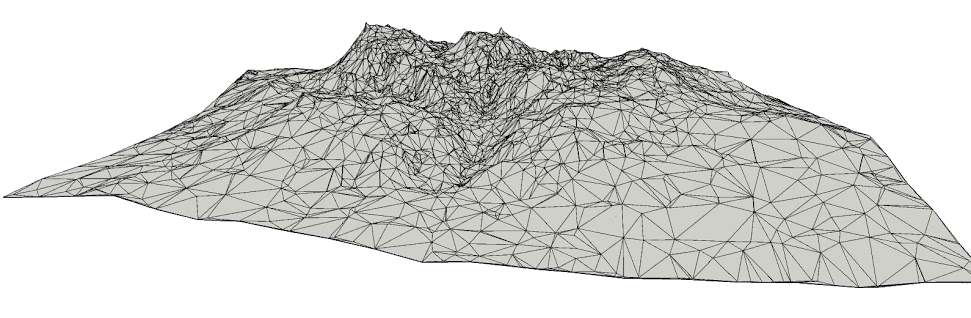
\includegraphics[width=0.7\linewidth]{Figures/mesh}
	\caption{Esempio di superficie rappresentata tramite \textit{mesh} triangolare.}
\end{figure}
\begin{figure}
	\centering
	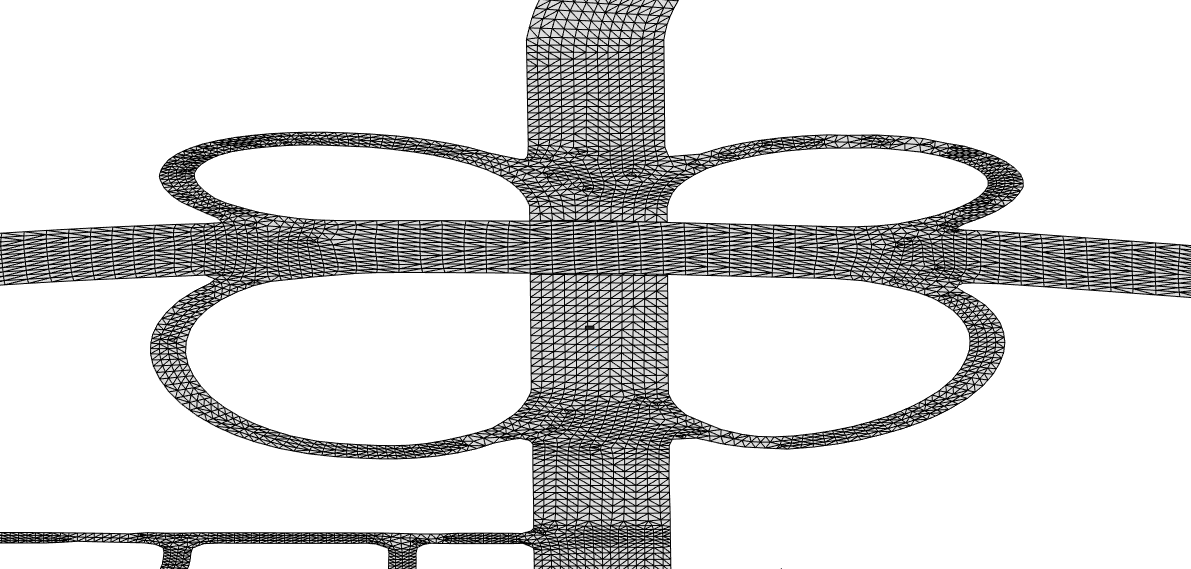
\includegraphics[width=0.7\linewidth]{Figures/mesh_1}
	\caption{Intersezione stradale rappresentata tramite \textit{mesh} triangolare.}
\end{figure}

Come verrà richiamato nelle conclusioni, l'importanza di definire uno \textit{standard} per il formato \ac{RDF} è di cruciale importanza. In questo modo si potrà creare un generatore di \textit{parser} con una grammatica e un lessico ben definiti, nonché aumentarne l'efficienza e la stabilità.
\chapter{Lo pneumatico}
\label{Pneumatico}
%
Gli pneumatici sono probabilmente i componenti più complessi di un'auto in quanto combinano decine di componenti che devono essere formati, assemblati e combinati assieme. Il successo del prodotto finale dipende dalla loro capacità di fondere tutti i componenti separati in un prodotto dal materiale coeso che soddisfa le esigenze del conducente \cite{rill}. Essi sono caratterizzati da un comportamento altamente non lineare con una forte dipendenza da diversi fattori costruttivi e ambientali.
%
\section{Geometria}
Quando si fa riferimento ai dati puramente geometrici, viene utilizzata una forma abbreviata della notazione completa prevista dall'ente di normazione \ac{ETRTO}. Assumendo di avere un pneumatico generico la notazione che identificherà la geometria sarà del tipo $a$ / $b$ R $c$. Dove:
\begin{itemize}
	\item $a$ rappresenta larghezza nominale dello pneumatico nel punto più largo;
	\item $b$ rappresenta percentuale dell'altezza della spalla dello pneumatico in relazione alla larghezza dello stesso;
	\item $c$ rappresenta il diametro dei cerchi ai quali lo pneumatico si adatta.
\end{itemize}
Si prenda come esempio la seguente denominazione \ac{ETRTO}: 195/55R16. La larghezza nominale dello pneumatico è di circa 195 mm nel punto più largo, l'altezza della spalla corrisponde al 55\% della larghezza $-$ ovvero 107 mm $-$ e il diametro dei cerchi ai quali lo pneumatico si adatta è di 16 pollici. Con questa notazione è possibile calcolare direttamente il diametro esterno teorico dello pneumatico tramite una delle seguenti formule:
%
\begin{equation}
\phi_e = \frac{2ab}{25.4}+c \quad \text{[in]} \qquad
\end{equation}
\begin{equation}
\phi_e = 2ab+25.4c \quad \text{[mm]}
\end{equation}
%
Riprendendo l'esempio usato sopra, il diametro esterno risulterà dunque 24.44 in o 621 mm.\\
Meno comunemente usato negli USA e in Europa (ma spesso in Giappone) è una notazione che indica l'intero diametro del pneumatico invece delle proporzioni dell'altezza della spalla laterale, quindi non secondo \ac{ETRTO}. Per fare lo stesso esempio, un cerchio da 16 pollici avrebbe un diametro di 406 mm. L'aggiunta del doppio dell'altezza del pneumatico (2$\times$107 mm) produce un diametro totale di 620 mm. Quindi, un pneumatico 195/55R16 potrebbe in alternativa essere etichettato come 195/620R16. Anche se queste due notazioni sono teoricamente ambigue, in pratica possono essere facilmente distinte perché l'altezza della parete laterale di uno pneumatico automobilistico è in genere molto inferiore alla larghezza. Quindi, quando l'altezza è espressa come percentuale della larghezza, è quasi sempre inferiore al 100\% (e certamente meno del 200\%). Al contrario, i diametri degli pneumatici del veicolo sono sempre superiori a 200 mm. Pertanto, se il secondo numero è superiore a 200, allora è quasi certo che viene utilizzata la notazione giapponese, se è inferiore a 200 allora viene utilizzata la notazione USA/europea.

\begin{figure}[h]
	\centering
	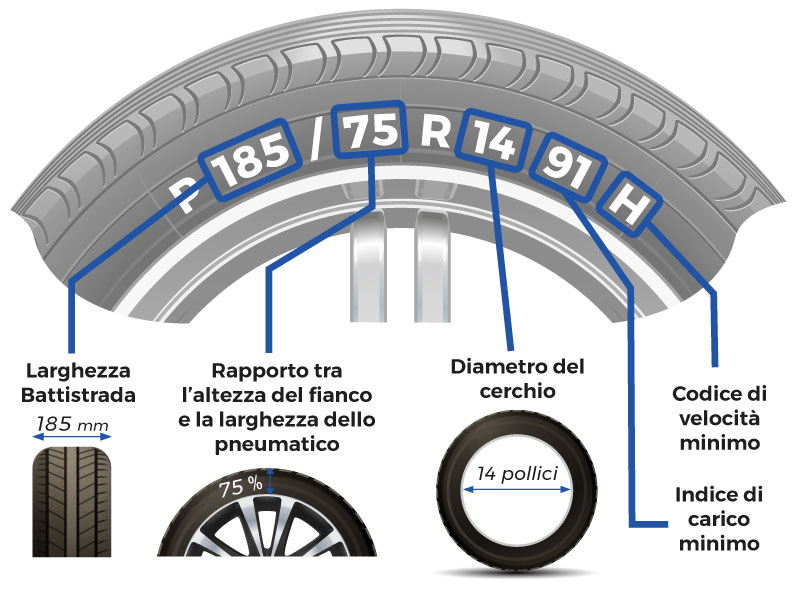
\includegraphics[width=0.7\linewidth]{Figures/tire_measures}
	\caption{Esempio di misure, secondo la notazione ETRTO, riportate sulla spalla dello pneumatico.}
	\label{tiremeasures}
\end{figure}
%
\section{Modelli di pneumatico}
Le forze di contatto tra la superficie stradale e lo pneumatico possono essere descritte da un vettore di forza risultante applicato in un punto specifico dell'impronta di contatto e da una coppia risultante, come illustrato nella \figurename{  \ref{tireforces}}.

\begin{figure}[h!]
	\centering
	\begin{subfigure}{0.4\linewidth}
		$F_x$ \quad forza longitudinale\\
		$F_y$ \quad forza laterale\\
		$F_z$ \quad forza verticale\\
		$T_x$ \quad coppia di sovrasterzo\\
		$T_y$ \quad resistenza al rotolamento\\
		$T_z$ \quad coppia di autoallineamento
	\end{subfigure}
	\begin{subfigure}{0.4\linewidth}
		\centering
		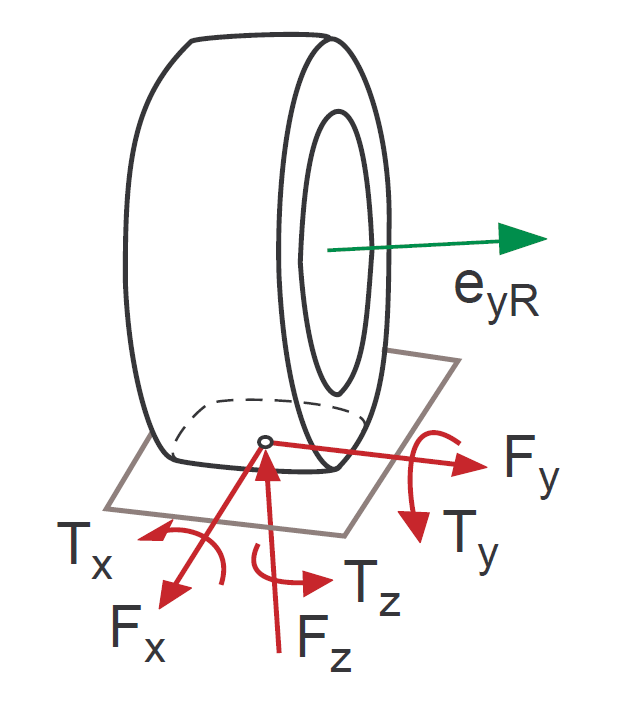
\includegraphics[width=\linewidth]{Figures/tire_forces}
	\end{subfigure}
\caption{Forze e coppie generate dal contatto pneumatico/strada.}
Da: \citeauthor{Rill}, \citetitle{Rill}.
\label{tireforces}
\end{figure}
%
Come componenti cruciali per la movimentazione dei veicoli e il comportamento di guida, le forze degli pneumatici richiedono particolare attenzione soprattutto perché deve essere considerato anche il comportamento non stazionario. Attualmente, è possibile suddividere i modelli di pneumatico in tre gruppi:
\begin{itemize}
	\item modelli matematici;
	\item modelli fisici;
	\item combinazione dei precedenti.
\end{itemize}

La prima tipologia di modello tenta di rappresentare le caratteristiche fisiche dello pneumatico attraverso una descrizione puramente matematica. Pertanto, questo tipo di modelli parte da un curve caratteristiche ricavate sperimentalmente e cercano di derivare un comportamento approssimativo dall'interpolazione di un grande insieme di dati. Un esempio ben noto di questo approccio è il \textbf{modello di Pacejka} o \textbf{\textit{Magic Formula}} \cite{hans}. Questo tipo di modellazione è adatta per la simulazione di guida in cui il comportamento di interesse è per lo più la guidabilità del veicolo e le frequenze di uscita sono ben al di sotto delle frequenze di risonanza della cintura dello pneumatico. I modelli fisici o i modelli ad alta frequenza, come i modelli agli elementi finiti, sono in grado di rilevare fenomeni di risonanza a frequenza più elevata. Ciò permette di valutare il comfort di guida di un veicolo. Dal punto di vista del calcolo, i modelli fisici complessi richiedono molto tempo al calcolatore per essere risolti, nonché di molti dati, al contrario dei più veloci modelli matematici, che richiedono un'accurata pre-elaborazione dei dati sperimentali. La terza tipologia di modelli consiste in un'estensione dei modelli matematici attraverso le leggi fisiche al fine di coprire una gamma di frequenza più ampia.

Il modello di pneumatico sviluppato nel modello di veicolo e il tipo di interfaccia di pneumatico/strada presentato da \citeauthor{Larcher} in \cite{Larcher} si basa sulla \textit{Magic Formula} 6.2.
%
\subsection{Il modello di Pacejka}
Uno dei modelli di pneumatici più utilizzati è il cosiddetto modello \textit{Magic Formula} sviluppato da \citeauthor{bakker} in \cite{bakker}. Questo modello è stato poi rivisto e l'ultima versione è riportata in \cite{hans}. Il modello \textit{Magic Formula} consiste in una pura descrizione matematica del rapporto input-output del contatto pneumatico/strada. Questa formulazione collega le variabili di forza con lo slip rigido del corpo che vengono trattati nelle sezioni successive. La forma generale della funzione di descrizione può essere scritta come:
%
\begin{equation}
y(x) = D\sin\{C\arctan[B(x + S_h ) - E(B(x + S_h ) - \arctan(B(x + S_h )))]\} + S_v
\end{equation}
%
dove i fattori rappresentano:
\begin{itemize}
	\item $B$ la rigidezza;
	\item $C$ la forma;
	\item $D$ il valore massimo della forza o coppia;
	\item $E$ la curvatura in corrispondenza del valore massimo;
	\item $S_v$ lo spostamento in verticale della curva caratteristica;
	\item $S_h$ lo spostamento in orizzontale della curva caratteristica.
\end{itemize}
e dove $y(x)$ può rappresentare la forza longitudinale $F_x$ , la forza laterale $F_y$ o la coppia di autoallineamento $M_z$, mentre $x$ è la componente di slip corrispondente. In \figurename{ \ref{pacejka}} sono illustrate le curve caratteristiche generiche degli pneumatici derivate con il metodo della \textit{Magic Formula}.\\
Per poter utilizzare la \textit{Magic Formula} è necessario conoscere:
\begin{itemize}
	\item la geometria dello pneumatico;
	\item lo slittamento (o \textit{slip});
	\item la forza verticale applicata allo pneumatico;
	\item la penetrazione in corrispondenza del punto di contatto e la sua derivata nel tempo;
	\item l'inclinazione tra piano strada e sistema di riferimento del centro ruota (angolo di camber relativo).
\end{itemize}
Ed è proprio nell'inclinazione tra piano strada e sistema di riferimento del centro ruota che si porrà una maggiore attenzione in quanto elemento fondamentale per ricavare l'effettivo punto di contatto dell'interazione pneumatico/strada.
%
\begin{figure}[h]
	\centering
	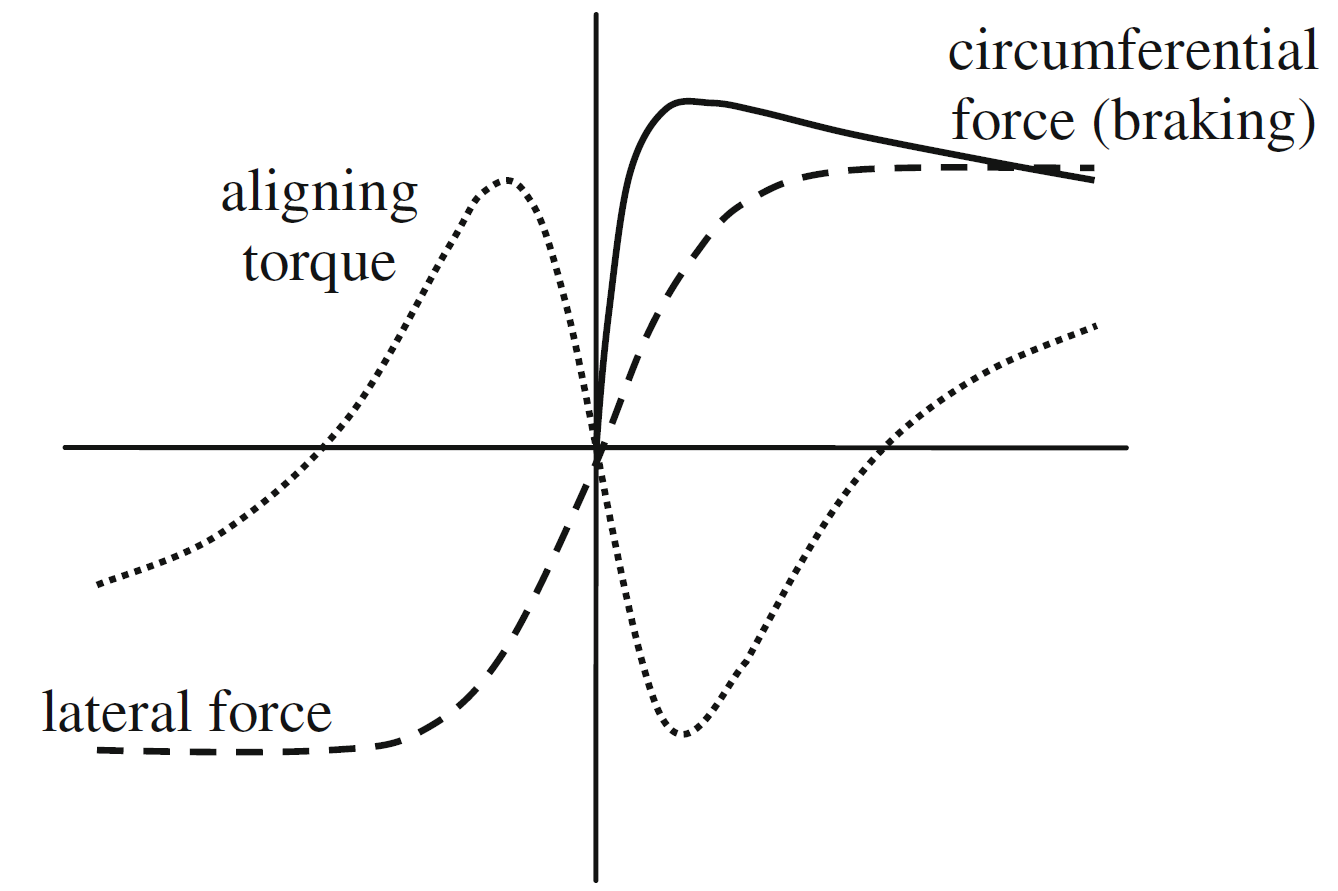
\includegraphics[width=0.58\linewidth]{Figures/pacejka}
	\caption{Curve caratteristiche generiche degli pneumatici derivate con il metodo della \textit{Magic Formula}.}
	Da: \citeauthor{Schramm}, \citetitle{Schramm}.
	\label{pacejka}
\end{figure}
%
\section{Contatto con la superficie stradale}
%
Si analizzaranno ora le quattro metodologie di complessità cresciente per ricavare l'inclinazione del piano locale e i punti di contatto sulla superficie stradale $P_{PL}$, nonché sulla circonferenza del disco indeformabile $P_{MF}$ dove effettivamente agiranno le forze ricavate mediante la \textit{Magic Formula}. Dapprima si utilizzerà un metodo a disco singolo presentato in \cite{Rill}, successivamente si passerà ad un modello a più dischi, così da coprire una superficie stradale maggiore e avere quindi risultati più precisi, soprattutto in prossimità di variazioni repentine del manto stradale.
%
\subsection{Modello di pneumatico a disco singolo}
%
\subsubsection{Contatto di Rill}
\label{Contatto_Rill}
%
\paragraph{Piano locale}
La posizione e l'orientamento della ruota in relazione al sistema fissato a terra sono dati dalla terna di riferimento del vettore ruota $RF_{wh}$, che viene calcolata istante per istante risolvendo le equazioni dinamiche del sistema ottenuto nel Capitolo 2 in \cite{Larcher}. Supponendo che il profilo stradale sia rappresentato da una funzione arbitraria a due coordinate spaziali del tipo: 
%
\begin{equation}
z=z(x,y)
\end{equation}
%
su una superficie irregolare, il punto di contatto con il piano locale $P_{PL}$ non può essere calcolato direttamente. Nel metodo a disco singolo presentato in \cite{Rill} da \citeauthor{Rill}, come prima approssimazione si identifica un punto di contatto $P^\star$ come una semplice traslazione del centro ruota $M$:
%
\begin{equation}
P^\star = M-R_0\textbf{\textit{e}}_{zC}
\begin{bmatrix}
x^\star\\
y^\star\\
z^\star
\end{bmatrix}
\end{equation}
%
dove $R_0$ è il raggio dello pneumatico indeformato ed $\textbf{\textit{e}}_{zC}$ è il vettore unitario che definisce l'asse $z_C$ del sistema di riferimento della ruota.

\begin{figure}[h]
	\centering
	\begin{subfigure}{0.45\linewidth}
		\centering
		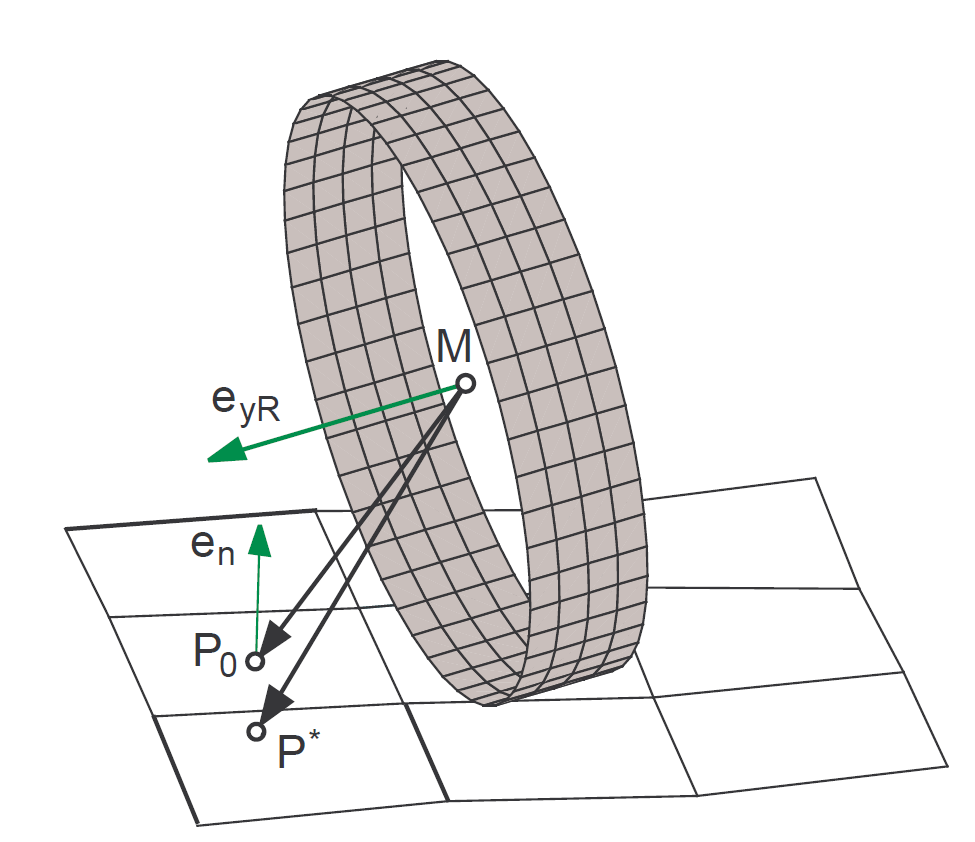
\includegraphics[width=\linewidth]{Figures/contact_geometry_1}
	\end{subfigure}
	\begin{subfigure}{0.35\linewidth}
		\centering
		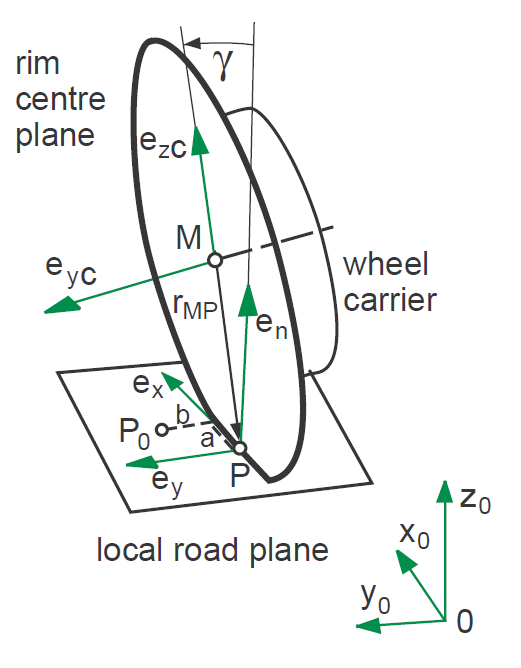
\includegraphics[width=\linewidth]{Figures/contact_geometry_2}
	\end{subfigure}
	\caption{Geometria del contatto pneumatico-strada.}
	Da: \citeauthor{Rill}, \citetitle{Rill}.
	\label{contactgeometry}
\end{figure}

La prima stima del sistema di riferimento del punto di contatto $RF_{P^\star}$ è una terna con origine in $P^\star$ e la medesima orientazione degli assi del sistema di riferimento della ruota. Si noti dunque che l'origine di $RF_{P^\star}$ corrisponde alla proiezione lungo l'asse $z_C$ del sistema di riferimento della ruota.

\begin{equation}
RF_{P^\star} = \left[
\begin{array}{ccc|c}
& & & x^\star\\
\multicolumn{3}{c|}{\multirow{3}{*}{\raisebox{20mm}{\scalebox{1.5}{$[R_{RF_{wh}}]$}}}} & y^\star\\
& & & z^\star\\ \hline
0 & ~~0 & 0 & 1
\end{array}\right]
\end{equation}\\

Al fine di ottenere una buona approssimazione del piano strada locale in termini di inclinazione longitudinale e laterale, sono stati utilizzati i quattro punti di campionamento $(Q^\star_1, Q^\star_2, Q^\star_3, Q^\star_4)$, rappresentati graficamente in \figurename{ \ref{localtrack}}. I punti di campionamento sono definiti nel sistema di riferimento temporaneo del punto di contatto $RF_{P^\star}$ e lo spostamento longitudinale e laterale sono definiti dall'origine, ovvero dallo stesso $P^\star$. I vettori di spostamento sono definiti come:
%
\begin{equation}
\begin{split}
\textbf{\textit{r}}_{Q^\star_{1,2}} = \pm \Delta x \textbf{\textit{e}}_{xP^\star} = \pm \Delta x \textbf{\textit{e}}_{xC} \\
\textbf{\textit{r}}_{Q^\star_{3,4}} = \pm \Delta y \textbf{\textit{e}}_{yP^\star} = \pm \Delta y \textbf{\textit{e}}_{yC}
\end{split}
\end{equation}
%
e quindi, i quattro punti di campionamento sono:
%
\begin{equation}
\begin{split}
Q^\star_{1,2} = P^\star \pm \textbf{\textit{r}}_{Q^\star_{1,2}} = P^\star \pm \Delta x \textbf{\textit{e}}_{xC} \\
Q^\star_{3,4} = P^\star \pm \textbf{\textit{r}}_{Q^\star_{3,4}} = P^\star \pm \Delta y \textbf{\textit{e}}_{yC}
\end{split}
\end{equation}
%
Al fine di campionare il terreno nel modo più efficace possibile, le distanze di $\Delta x$ e $\Delta y$, dell'equazione precedente, vengono regolate in base al raggio del pneumatico indeformato $R_0$ e alla larghezza del pneumatico $B$. I valori di queste due quantità possono essere trovate in \cite{Rill} e sono $\Delta x = 0.1 R_0$ e $\Delta x = 0.3 B$. Attraverso questa definizione, si può ottenere un comportamento sufficientemente realistico durante la simulazione.

\begin{figure}[h]
	\centering
	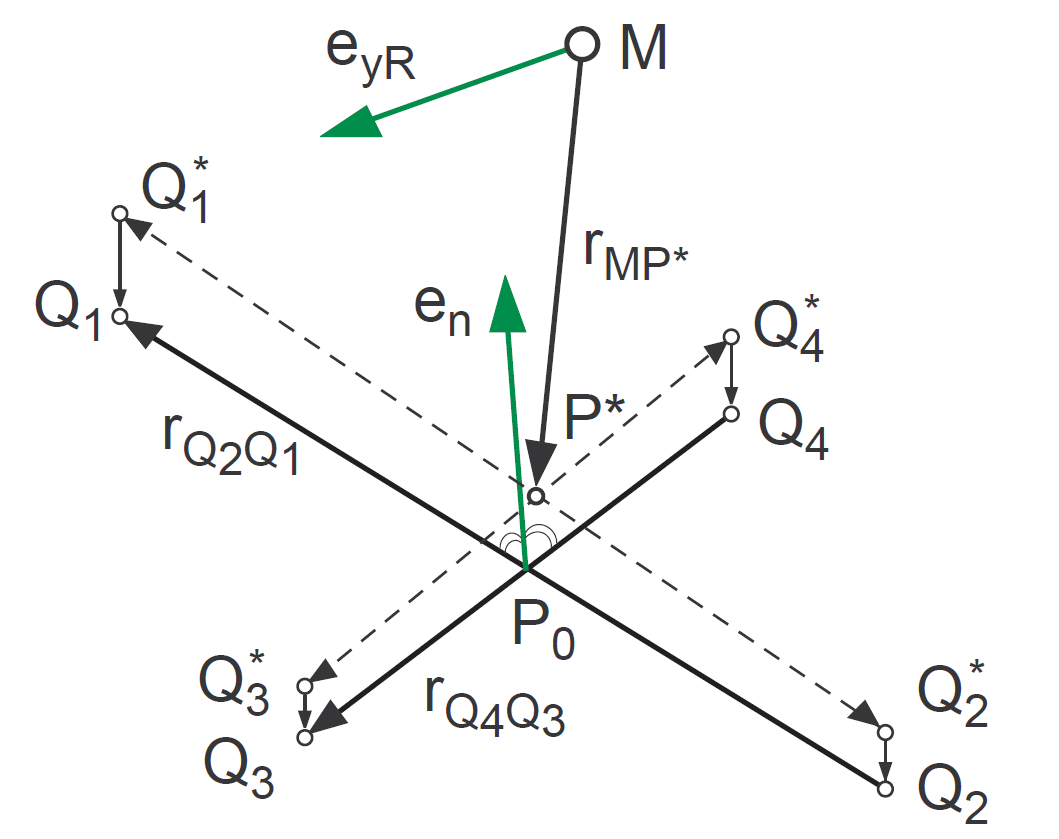
\includegraphics[width=0.5\linewidth]{Figures/local_track}
	\caption{Punti campionati nel piano locale della superficie stradale.}
	Da: \citeauthor{Rill}, \citetitle{Rill}.
	\label{localtrack}
\end{figure}

Ora la componente $z$ in corrispondenza dei quattro punti campione viene valutata attraverso la funzione $z(x,y)$ precedentemente definita. Quindi, aggiornando la terza coordinata dei punti di campionamento $Q^\star_i$, si ottenengono i corrispondenti punti campione $Q_i$ sulla superficie. La linea fissata dai punti $Q_1$, $Q_2$ e $Q_3$, $Q_4$, può ora essere utilizzata per definire la normale al piano strada locale (\figurename{ \ref{localplane}}). Pertanto, il vettore normale è definito come:
%
\begin{equation}
\textbf{\textit{e}}_n = \frac{\textbf{\textit{r}}_{Q_1 Q_2} \times \textbf{\textit{r}}_{Q_4 Q_3}}{|\textbf{\textit{r}}_{Q_1 Q_2} \times \textbf{\textit{r}}_{Q_4 Q_3}|}
\label{normale}
\end{equation}
%
Ora, i versori $\textbf{\textit{e}}_x$ ed $\textbf{\textit{e}}_y$, che descrivono l'inclinazione del piano locale nel possono essere ottenuti dalle seguenti equazioni:
%
\begin{equation}
\textbf{\textit{e}}_x = \frac{\textbf{\textit{e}}_{yC}\times\textbf{\textit{e}}_{n}}{|\textbf{\textit{e}}_{yC}\times\textbf{\textit{e}}_{n}|}
\qquad
\textbf{\textit{e}}_{y} = \textbf{\textit{e}}_{n}\times\textbf{\textit{e}}_{x}
\label{terna}
\end{equation}
%
dove sono $\textbf{\textit{r}}_{Q_2 Q_1}$ e $\textbf{\textit{r}}_{Q_4 Q_3}$ sono i vettori che puntano rispettivamente da $Q_1$ a $Q_2$ e da $Q_3$ a $Q_4$. Applicando la \eqref{terna} è ora possibile calcolare i vettori unitari $\textbf{\textit{e}}_{x}$ e $\textbf{\textit{e}}_{y}$ del piano locale di contatto. Per definire univocamente il piano strada, oltre alla normale calcolata in \eqref{normale}, viene utilizzato il punto $P_n$ dato dal valore medio delle tre coordinate spaziali dei quattro punti campione.
%
\begin{equation}
P_n = \frac{1}{4}\begin{bmatrix}
\sum_{i=1}^{4} x_i \\
\sum_{i=1}^{4} y_i \\
\sum_{i=1}^{4} z_i
\end{bmatrix}
\end{equation}
%
\paragraph{Punti di contatto}
\label{Punti_contatto_rill}
È infine necessario ricondursi alle condizioni tali per cui il modello di Pacejka è valido trovando il punto di contatto sul piano strada locale $P_{PL}$ e il punto di contatto sulla circonferenza del disco indeformabile $P_{MF}$ dove effettivamente agiranno le forze ricavate mediante la \textit{Magic Formula}. Si troverà dapprima la componente della normale al piano strada $\textbf{\textit{e}}_{n_{XZ}}$ sul piano in cui giace il singolo disco indeformabile. $P_{MF}$ sarà dunque trovato a partire dal centro ruota $M$, moltiplicando scalarmente il versore $-\textbf{\textit{e}}_{n_{XZ}}$ per il raggio del disco indeformabile $R_0$, ovvero:
%
\begin{equation}
P_{MF} = -R_0\textbf{\textit{e}}_{n_{XZ}}
\label{puntoMF}
\end{equation}
%
Come illustrato in \figurename{ \ref{localplane}}, il punto di contatto sul piano strada locale $P_{PL}$ viene invece calcolato sfuttando un algoritmo di intersezione piano-raggio (che si tratterà nel Capitolo \ref{Geom_Algos}). $P_{PL}$ giacerà dunque sulla proiezione in direzione $-\textbf{\textit{e}}_{n_{XZ}}$ del punto $M$ sulla retta individuata dal punto $P_n$ e normale $\textbf{\textit{e}}_{n_{XZ}}$.

\begin{figure}[h]
	\centering
	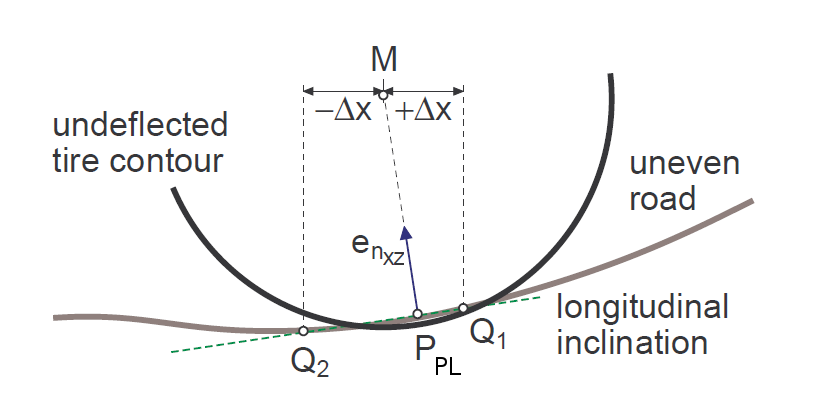
\includegraphics[width=0.6\linewidth]{Figures/local_plane_PL}
	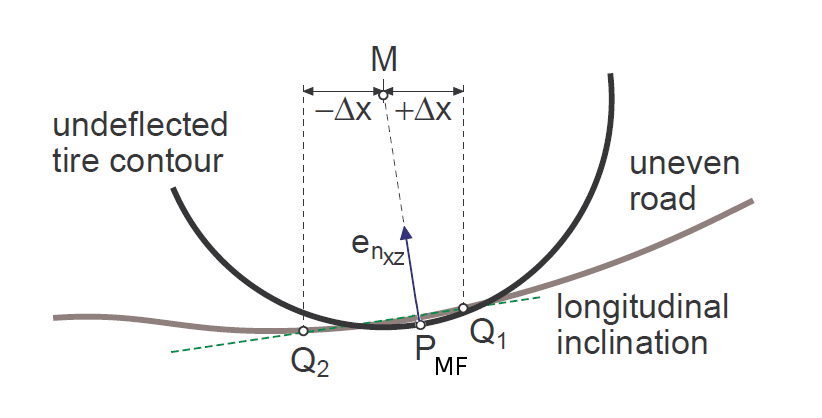
\includegraphics[width=0.6\linewidth]{Figures/local_plane_MF}
	\caption{Punti di contatto $P_{PL}$ e $P_{MF}$ in relazione alla normale $\textbf{\textit{e}}_{n_{XZ}}$.}
	\label{localplane}
\end{figure}

Infine si può mettere assieme tutte le componenti del piano di riferimento del punto di contatto $P_{MF}$ ottenendo il relativo sistema di riferimento:
%
\begin{equation}
RF_{MF} = \left[
\begin{array}{ccc|c}
& & & x_{P_{MF}}\\
\multirow{3}{*}{\raisebox{20mm}{\scalebox{1.5}{$\left[\textbf{\textit{e}}_x\right]$}}} & \multirow{3}{*}{\raisebox{20mm}{\scalebox{1.5}{$\left[\textbf{\textit{e}}_y\right]$}}} & \multirow{3}{*}{\raisebox{20mm}{\scalebox{1.5}{$\left[\textbf{\textit{e}}_z\right]$}}} & y_{P_{MF}}\\
& & & z_{P_{MF}}\\ \hline
0 & 0 & 0 & 1
\end{array}\right]
\end{equation}\\
Attraverso questo approccio, la normale del piano strada locale $\textbf{\textit{e}}_{n}$ insieme al punto di contatto sul piano strada locale $P_{PL}$ e al punto di contatto sulla circonferenza del disco indeformabile $P_{MF}$, sono in grado di rappresentare l'irregolarità della strada in modo soddisfacente ma comunque approssimativo, infatti, bordi taglienti o discontinuità del manto stradale saranno involontariamente filtrate da questo approccio.

Nel caso specifico di questo lavoro la superficie stradale non è rappresentata da una funzione del tipo $z(x,y)$ ma bensì da una serie di triangoli. Questo comporta l'impossibilità di valutare la terza coordinata dei punti di campionamento $Q_i^\star$. Per sopperire a questo problema si utilizzerà l'algoritmo per l'intersezione tra raggio e triangolo presentato nel Capitolo \ref{Geom_Algos}. Si definirano dunque i punti di origine dei raggi direttamente nel sistema di riferimento della ruota $RF_{wh}$ come:
\begin{equation}
\begin{split}
Q^\star_{1,2} = M \pm \textbf{\textit{r}}_{Q^\star_{1,2}} = P^\star \pm \Delta x \textbf{\textit{e}}_{xC} \\
Q^\star_{3,4} = M \pm \textbf{\textit{r}}_{Q^\star_{3,4}} = P^\star \pm \Delta y \textbf{\textit{e}}_{yC}
\end{split}
\end{equation}
dai quali partiranno i raggi con direzione $-z_C$ che intersecheranno la \textit{mesh} nei punti $(Q_1, Q_2, Q_3, Q_4)$.
%
\subsubsection{Contatto ponderato in base all'area d'intersezione}
%
\paragraph{Piano locale}
Alternativamente a quello appena visto, si può utilizzare un modello di contatto ponderato in base all'area di intersezione. In altre, parole si andrà a valutare triangolo per triangolo l'intersezione con il disco indeformabile. Prima di tutto di intersecherà il triangolo nello spazio con il piano in cui giace il disco trovando dunque un segmento. Successivamente si valuterà l'intersezione di questo segmento con il disco, calcolando l'area tra il segmento stesso e il semicerchio inferiore del disco.

\begin{figure}
	\centering
	\begin{tikzpicture}
	\def\axisl{3};
	\def\zd{1.9};
	\draw[-stealth] (-\axisl,0) -- (\axisl,0) node[below]{$x_C$};
	\draw[-stealth] (0,-\axisl) -- (0,\axisl) node[left]{$z_C$};
	\draw[thick] (0,0) circle (2);
	
	\draw[] (-1,-0.8) node[above]{$A$} --  (1,-1.1) node[above]{$B$};
	\draw[dashed] (-1,-0.8) --  (-1,-2*0.866) node[below]{$A'$};
	\draw[dashed] (1,-1.1) --  (1,-2*0.866) node[below]{$B'$};
	
	\draw[] (-1,-0.8)  --  (-2.5,-1.1);
	\draw[] (1,-1.1)  --  (2.5,-1.1) node[below]{\textit{Mesh}};	
	\end{tikzpicture}
	\caption{Dato un generico triangolo che, intersecando il piano in cui giace il disco, crea il segmento dato dai punti $A$ e $B$. L'area di intersezione associata al triangolo è l'area della regione racchiusa dai segmenti $B'B$, $AB$, $AA'$ e dall'arco di cisconferenza $A'B'$.}
\end{figure}
\begin{figure}
	\centering
	\begin{tikzpicture}
	\def\axisl{3};
	\def\zd{1.9};
	\draw[-stealth] (-\axisl,0) -- (\axisl,0) node[below]{$x_C$};
	\draw[-stealth] (0,-\axisl) -- (0,\axisl) node[left]{$z_C$};
	\draw[thick] (0,0) circle (2);
	
	\draw[] (-2.5,-1) -- (-1,-0.8) --  (0,-1.1) -- (1,-0.7) -- (2.5,-0.8) node[below]{\textit{Mesh}};
	\draw[dashed] (-1,-0.8) --  (-1,-2*0.866);
	\draw[dashed] (1,-0.7) --  (1,-2*0.866);
	\draw[]  (1.35,-0.8) node[below]{$D$};
	\draw[]  (0.5,-1.2) node[below]{$C$};
	\draw[]  (-0.5,-1.2) node[below]{$B$};
	\draw[]  (-1.3,-0.85) node[below]{$A$};
	\draw[-stealth] (1.5,-0.73) -- (1.55,-0.1) node[above]{\tiny$\vec{N}_D$};
	\draw[-stealth] (0.5,-0.9)  -- (0.2,-0.1) node[above]{\tiny$\vec{N}_C$};
	\draw[-stealth] (-0.5,-0.95) -- (-0.25,-0.1) node[above]{\tiny$\vec{N}_B$};
	\draw[-stealth] (-1.5,-0.87) -- (-1.6,-0.1) node[above]{\tiny$\vec{N}_A$};
	\end{tikzpicture}
	\caption{I versori normali $\vec{N}_A$, $\vec{N}_B$, $\vec{N}_C$ e $\vec{N}_D$ vengono pesati per l'area delle rispettive regioni d'interesezione $A$, $B$, $C$ e $D$.}
\end{figure}

Attraverso questa area si potrà pesare la normale alla faccia del triangolo considerato e quindi effettuare una media ponderata con tutti gli atri triangoli che insersecano il disco, ovvero:
%
\begin{equation}
\textbf{\textit{e}}_n = \sum_{i=0}^{N_T}A_i\textbf{\textit{e}}_{n_i}
\label{ponderata}
\end{equation}
%
dove:
\begin{itemize}
	\item $N_T$ è il numero di triangoli all'interno della \ac{BB} rappresentante l'ombra dello pneumatico;
	\item $\textbf{\textit{e}}_n$ è il versore normale risultante;
	\item $\textbf{\textit{e}}_{n_i}$ è il versore normale dell'$i$-esimo triangolo;
	\item $A_i$ l'area tra il segmento creato dall'intersezione piano-trangolo e il semicerchio inferiore del disco dell'$i$-esimo triangolo.
\end{itemize}

Questo metodo è ovviamente utilizzabile solo nel caso di strada rappresentata tramite \textit{mesh} triangolare. A differenza dal modello di \cite{Rill}, permette di non approssimare la superficie stradale mediante soli quattro punti ma invece di avere una rappresentazione che sfrutta tutti i dati messi a disposizione dalla discretizzazione del manto stradale.
%
\paragraph{Punti di contatto}
Per trovare il punto di contatto con la \textit{mesh} $P_{PL}$ e il punto di contatto sulla circonferenza del disco indeformabile $P_{MF}$ precedentemente definiti, si andrà a ripetere l'operazione in \ref{Punti_contatto_rill} per trovare la componente della normale al piano strada $\textbf{\textit{e}}_{n_{XZ}}$ sul piano in cui giace il singolo disco indeformabile. A differenza del modello di contatto di Rill, non si ha ora una definizione univoca del piano strada locale. Infatti, l'unica componente ad ora conoscita è il versore risultante normale al terreno $\textbf{\textit{e}}_n$. Per ricavare il punto di contatto sulla circonferenza del disco indeformabile $P_{MF}$ si utilizzerà la \eqref{puntoMF}, mentre per il punto sulla \textit{mesh} $P_{PL}$ si andrà ad utilizzare un algoritmo d'intersezione tra raggio e la superficie stradale, dove l'origine del raggio sarà il centro ruota e la direzione $-\textbf{\textit{e}}_{n_{XZ}}$.
%
\subsection{Modello di pneumatico a più dischi}
%
Nel modello a più dischi, lo pneumatico sarà rappresentato da più dischi rigidi indeformabili disposti uniformemente lungo la sezione dello stesso. Essi potranno avere raggio uguale o diverso l'uno dall'altro, in modo da rappresentare una forma specifica dello pneumatico.

\begin{figure}[h!]
	\hfill
	\begin{subfigure}{.3\textwidth}
		\centering
		\begin{tikzpicture}
		\def\axisl{2};
		\def\zd{1};
		\draw[-stealth] (-0.8*\axisl,0) -- (0.8*\axisl,0) node[below]{$y_C$};
		\draw[-stealth] (0,-1.3*\axisl) -- (0,1.3*\axisl) node[left]{$z_C$};
		
		\draw[line width=0.35mm] (-1,-\axisl/\zd) -- (-1,\axisl/\zd);
		\draw[line width=0.35mm] (-0.75,-\axisl/\zd) -- (-0.75,\axisl/\zd);
		\draw[line width=0.35mm] (-0.5,-\axisl/\zd) -- (-0.5,\axisl/\zd);
		\draw[line width=0.35mm] (-0.25,-\axisl/\zd) -- (-0.25,\axisl/\zd);
		
		\draw[line width=0.35mm] (0,-\axisl/\zd) -- (0,\axisl/\zd);

		\draw[line width=0.35mm] (0.25,-\axisl/\zd) -- (0.25,\axisl/\zd);
		\draw[line width=0.35mm] (0.5,-\axisl/\zd) -- (0.5,\axisl/\zd);
		\draw[line width=0.35mm] (0.75,-\axisl/\zd) -- (0.75,\axisl/\zd);
		\draw[line width=0.35mm] (1,-\axisl/\zd) -- (1,\axisl/\zd);
		\end{tikzpicture}
		\caption{Raggio uniforme}
	\end{subfigure}
	\hfill
	\begin{subfigure}{.3\textwidth}
		\centering
		\begin{tikzpicture}
		\def\axisl{2};
		\def\zd{1};
		\draw[-stealth] (-0.8*\axisl,0) -- (0.8*\axisl,0) node[below]{$y_C$};
		\draw[-stealth] (0,-1.3*\axisl) -- (0,1.3*\axisl) node[left]{$z_C$};
		
		\draw[line width=0.35mm] (-1,-\axisl/\zd+0.5) -- (-1,\axisl/\zd-0.5);
		\draw[line width=0.35mm] (-0.75,-\axisl/\zd+0.5-0.5*1.41/2) -- (-0.75,\axisl/\zd-0.5+0.5*1.41/2);
		\draw[line width=0.35mm] (-0.5,-\axisl/\zd) -- (-0.5,\axisl/\zd);
		\draw[line width=0.35mm] (-0.25,-\axisl/\zd) -- (-0.25,\axisl/\zd);
		
		\draw[line width=0.35mm] (0,-\axisl/\zd) -- (0,\axisl/\zd);
		
		\draw[line width=0.35mm] (0.25,-\axisl/\zd) -- (0.25,\axisl/\zd);
		\draw[line width=0.35mm] (0.5,-\axisl/\zd) -- (0.5,\axisl/\zd);
		\draw[line width=0.35mm] (0.75,-\axisl/\zd+0.5-0.5*1.41/2) -- (0.75,\axisl/\zd-0.5+0.5*1.41/2);
		\draw[line width=0.35mm] (1,-\axisl/\zd+0.5) -- (1,\axisl/\zd-0.5);
		\end{tikzpicture}
		\caption{Spalla raccordata}
	\end{subfigure}
	\hfill
		\begin{subfigure}{.3\textwidth}
		\centering
		\begin{tikzpicture}
		\def\axisl{2};
		\def\zd{1};
		\draw[-stealth] (-0.8*\axisl,0) -- (0.8*\axisl,0) node[below]{$y_C$};
		\draw[-stealth] (0,-1.3*\axisl) -- (0,1.3*\axisl) node[left]{$z_C$};
		
		\draw[line width=0.35mm] (-1,-\axisl/\zd+0.25) -- (-1,\axisl/\zd-0.25);
		\draw[line width=0.35mm] (-0.75,-\axisl/\zd) -- (-0.75,\axisl/\zd);
		\draw[line width=0.35mm] (-0.5,-\axisl/\zd+0.1) -- (-0.5,\axisl/\zd-0.1);
		\draw[line width=0.35mm] (-0.25,-\axisl/\zd+0.2) -- (-0.25,\axisl/\zd-0.2);
		
		\draw[line width=0.35mm] (0,-\axisl/\zd+0.3) -- (0,\axisl/\zd-0.3);
		
		\draw[line width=0.35mm] (0.25,-\axisl/\zd+0.2) -- (0.25,\axisl/\zd-0.2);
		\draw[line width=0.35mm] (0.5,-\axisl/\zd+0.1) -- (0.5,\axisl/\zd-0.1);
		\draw[line width=0.35mm] (0.75,-\axisl/\zd) -- (0.75,\axisl/\zd);
		\draw[line width=0.35mm] (1,-\axisl/\zd+0.25) -- (1,\axisl/\zd-0.25);
		\end{tikzpicture}
		\caption{Profilo personalizzato}
	\end{subfigure}
	\hfill
	\caption{Disposizione dei dischi.}
\end{figure}

Anche se questo modello di pneumatico è costituito da più dischi, il punto di contatto $P_{MF}$ utilizzato per valutare la formula di Pacejka verrà comunque considerato nel disco fittizio giacente sul piano $XZ$ dello pneumatico. Equivalentemente, anche il punto di contatto con la \textit{mesh} $P_{PL}$ verrà considerato nel mediesimo piano.

\begin{figure}[h!]
	\centering
	\begin{tikzpicture}
	\def\axisl{2};
	\def\zd{1};
	\draw[-stealth] (-0.8*\axisl,0) -- (0.8*\axisl,0) node[below]{$y_C$};
	\draw[-stealth] (0,-1.3*\axisl) -- (0,1.3*\axisl) node[left]{$z_C$};
	
	\draw[line width=0.35mm] (-0.75,-\axisl/\zd) -- (-0.75,\axisl/\zd);
	\draw[line width=0.35mm] (-0.25,-\axisl/\zd) -- (-0.25,\axisl/\zd);
	\draw[dashed, line width=0.5mm] (0,-\axisl/\zd) -- (0,\axisl/\zd);
	\draw[line width=0.35mm] (0.25,-\axisl/\zd) -- (0.25,\axisl/\zd);
	\draw[line width=0.35mm] (0.75,-\axisl/\zd) -- (0.75,\axisl/\zd);
	\end{tikzpicture}
	\caption{Pneumatico rappresentato da dischi a raggio uniforme. Notare il disco fittizio giacente sul piano $XZ$ in linea tratteggiata.}
\end{figure}

\begin{figure}[h!]
	\hfill
	\begin{subfigure}{.49\linewidth}
	\centering
	\begin{tikzpicture}
		\def\axisl{2};
		\def\zd{1};
		\draw[-stealth] (0,0) -- (0.6*\axisl,0) node[below]{$y_C$};
		\draw[-stealth] (0,0) -- (0,1.2*\axisl) node[left]{$z_C$};
		
		\draw[line width=0.5mm] (-0.75,-\axisl/\zd) -- (-0.75,\axisl/\zd);
		\draw[line width=0.5mm] (-0.25,-\axisl/\zd) -- (-0.25,\axisl/\zd);
		\draw[line width=0.5mm] (0.25,-\axisl/\zd) -- (0.25,\axisl/\zd);
		\draw[line width=0.5mm] (0.75,-\axisl/\zd) -- (0.75,\axisl/\zd);
		
		\draw[] (-2.2,-1.5) -- (-1,-1.8) --  (0,-1.5) -- (1,-1.6) -- (2.2,-1.5) node[below]{\textit{Mesh}};
		
		\draw[-stealth] (0.75,-\axisl/\zd-0.7) node[below]{\small$\vec{F}_{z_3}$} -- (0.75,-\axisl/\zd);
		\draw[-stealth] (0.25,-\axisl/\zd-1) node[below]{\small$\vec{F}_{z_2}$} -- (0.25,-\axisl/\zd);
		\draw[-stealth] (-0.25,-\axisl/\zd-0.8) node[below]{\small$\vec{F}_{z_1}$} -- (-0.25,-\axisl/\zd);
		\draw[-stealth] (-0.75,-\axisl/\zd-0.6) node[below]{\small$\vec{F}_{z_0}$} -- (-0.75,-\axisl/\zd);
	\end{tikzpicture}
	\end{subfigure}
\hfill
	\begin{subfigure}{.49\linewidth}
	\centering
	\begin{tikzpicture}
		\def\axisl{2};
		\def\zd{1};
		\draw[-stealth] (0,0) -- (0.6*\axisl,0) node[below]{$y_C$};
		\draw[-stealth] (0,0) -- (0,1.2*\axisl) node[left]{$z_C$};
		
		\draw[line width=0.5mm] (-0.75,-\axisl/\zd) -- (-0.75,\axisl/\zd);
		\draw[line width=0.5mm] (-0.25,-\axisl/\zd) -- (-0.25,\axisl/\zd);
		\draw[line width=0.5mm] (0.25,-\axisl/\zd) -- (0.25,\axisl/\zd);
		\draw[line width=0.5mm] (0.75,-\axisl/\zd) -- (0.75,\axisl/\zd);
		
		\draw[-stealth] (1,0.2) node[above right]{$M_x$} arc (10:300:1) ;
		
		\draw[] (-2.2,-1.5) -- (-1,-1.8) --  (0,-1.5) -- (1,-1.6) -- (2.2,-1.5) node[below]{\textit{Mesh}};
	\end{tikzpicture}
	\end{subfigure}
\hfill
\caption{Momento creato dalla morfologia del terreno.}
\end{figure}
%
\subsubsection{Contatto ponderato in base all'area d'instersezione}
\paragraph{Piano locale}
Analogamente al modello di pneumatico a singolo disco, si può effettuare la stessa operazione su ogni disco per trovare il versore normale risultante $\textbf{\textit{e}}_{n_{D_j}}$ relativo al contatto del $j$-esimo disco. La \eqref{ponderata} diventerà dunque:
%
\begin{equation}
\textbf{\textit{e}}_{n_{D_j}} = \sum_{i=0}^{N_T}A_i\textbf{\textit{e}}_{n_i}
\end{equation}
%
Per combinare assieme i versori normali $\textbf{\textit{e}}_{n_{D_j}}$ relativi ai dischi si effetturà una nuova media ponderata pesata questa volta sull'area totale all'interno del disco e sotto la superficie della \textit{mesh}. La formula sarà dunque:
%
\begin{equation}
\textbf{\textit{e}}_n = \sum_{j=0}^{N_D}A_{D_j}\textbf{\textit{e}}_{n_{D_j}}
\end{equation}
%
dove:
\begin{itemize}
	\item $N_D$ è il numero di dischi totali rappresentanti lo pneumatico;
	\item $\textbf{\textit{e}}_n$ è il versore normale risultante;
	\item $\textbf{\textit{e}}_{n_{D_j}}$ è il versore normale associato al $j$-esimo disco;
	\item $A_{D_j}$ l'area d'intersezione all'interno del disco e sotto la superficie della \textit{mesh} dell'$j$-esimo disco.
\end{itemize}

\begin{figure}
	\centering
	\tdplotsetmaincoords{70}{110}
	\tdplotsetrotatedcoords{90}{90}{0}
	\begin{tikzpicture}[tdplot_main_coords]
	
	\draw[-stealth] (0,0,0) -- (8,0,0) node[anchor=north east]{$x_C$};
	\draw[-stealth] (0,0,0) -- (0,3,0) node[anchor=north west]{$y_C$};
	\draw[-stealth] (0,0,0) -- (0,0,5) node[anchor=north west]{$z_C$};
	
	\def\r{4};
	\draw[-stealth] (0,1.6,-\r+0.5) -- (0,1.6,-\r+1.5);
	\draw[-stealth] (0,1.2,-\r+0.5-0.5*1.41/2) -- (0-0.1,1.2+0.1,-\r+1.5-0.5*1.41/2);
	\draw[-stealth] (0,0.8,-\r) -- (0,0.8,-\r+1);
	\draw[-stealth] (0,0.4,-\r) -- (0+0.1,0.4-0.1,-\r+1);
	\draw[-stealth] (0,0,-\r) -- (0+0.05,0-0.1,-\r+1);
	\draw[-stealth] (0,-0.4,-\r) -- (0,-0.4,-\r+1);
	\draw[-stealth] (0,-0.8,-\r) -- (0+0.1,-0.8+0.1,-\r+1);
	\draw[-stealth] (0,-1.2,-\r+0.5-0.5*1.41/2) -- (0,-1.2,-\r+1.5-0.5*1.41/2);
	\draw[-stealth] (0,-1.6,-\r+0.5) -- (0,-1.6,-\r+1.5);
	
	\begin{scope}[tdplot_rotated_coords]
	\tdplotdrawarc[tdplot_rotated_coords,thick]{(0,0,1.6)}{\r-0.5}{0}{360}{}{}
	
	\tdplotdrawarc[tdplot_rotated_coords,thick]{(0,0,1.2)}{\r-0.5+0.5*1.41/2}{3}{-228}{}{}
	\tdplotdrawarc[tdplot_rotated_coords, dashed,thick]{(0,0,1.2)}{\r-0.5+0.5*1.41/2}{3}{360-228}{}{}
	
	\tdplotdrawarc[tdplot_rotated_coords,thick]{(0,0,0.8)}{\r}{-9}{-217}{}{}
	\tdplotdrawarc[tdplot_rotated_coords, dashed,thick]{(0,0,0.8)}{\r}{-9}{360-217}{}{}
	
	\tdplotdrawarc[tdplot_rotated_coords,thick]{(0,0,0.4)}{\r}{-15}{-210}{}{}
	\tdplotdrawarc[tdplot_rotated_coords, dashed,thick]{(0,0,0.4)}{\r}{-15}{360-210}{}{}
	
	\tdplotdrawarc[tdplot_rotated_coords,thick]{(0,0,0)}{\r}{-15}{-210}{}{}
	\tdplotdrawarc[tdplot_rotated_coords, dashed,thick]{(0,0,0)}{\r}{-15}{360-210}{}{}
	
	\tdplotdrawarc[tdplot_rotated_coords,thick]{(0,0,-0.4)}{\r}{-15}{-210}{}{}
	\tdplotdrawarc[tdplot_rotated_coords, dashed,thick]{(0,0,-0.4)}{\r}{-15}{360-210}{}{}
	
	\tdplotdrawarc[tdplot_rotated_coords,thick]{(0,0,-0.8)}{\r}{-15}{-210}{}{}
	\tdplotdrawarc[tdplot_rotated_coords, dashed,thick]{(0,0,-0.8)}{\r}{-15}{360-210}{}{}
	
	\tdplotdrawarc[tdplot_rotated_coords,thick]{(0,0,-1.2)}{\r-0.5+0.5*1.41/2}{-17}{-205}{}{}
	\tdplotdrawarc[tdplot_rotated_coords, dashed,thick]{(0,0,-1.2)}{\r-0.5+0.5*1.41/2}{-17}{360-205}{}{}
	
	\tdplotdrawarc[tdplot_rotated_coords,thick]{(0,0,-1.6)}{\r-0.5}{-30}{-195}{}{}
	\tdplotdrawarc[tdplot_rotated_coords, dashed,thick]{(0,0,-1.6)}{\r-0.5}{-20}{360-195}{}{}
	\end{scope}
	\end{tikzpicture}
	\caption{Normali associate ai vari dischi dello pneumatico.}
\end{figure}

\paragraph{Punti di contatto}
Avendo ora a disposizione il versore normale risultante $\textbf{\textit{e}}_n$, si può ora trovare i punti $P_{MF}$ e $P_{PL}$ adottando il medesimo metodo utilizato in \ref{Contatto_Rill}. Si noti che anche se lo pneumatico è rapprensentato da più dischi, per ricondursi alle condizioni tali per cui il modello di Pacejka è valido, è necessario immaginare che ci sia sempre un disco fittizio giacente sul piano $XZ$ della ruota.
%
\subsubsection{Contatto tramite campionamento}
\paragraph{Piano locale}
Nel caso in cui la densità della \textit{mesh} sia troppo alta, effettuare il calcolo per il modello di contatto ponderato in base all'area d'instersezione precedentemente presentato, può essere molto dispendioso in termini di calcoli, e quindi di tempo. Per sopperire a questo problema, se il numero di triangoli è superiore ad un certo \textit{threshold}, si andrà a campionare la \textit{mesh} triangolare in corrispondenza del piano in cui giacciono i dischi. In particolare, per campionare la \textit{mesh} si sfrutterà l'algoritmo di intersezione tra raggio e triangolo che verrà presentato nel Capitolo \ref{Geom_Algos}. Attraverso questo algoritmo, suppenendo che il raggio abbia la stessa direzione dell'asse $z_C$, si andranno a memorizzare le normali alle faccie dei triangoli campionati. Il versore normale risultante $\textbf{\textit{e}}_n$ non verrà più calcolato mediante una media ponderata ma bensì attravarso una media semplice tra tutti i punti campionati lungo il disco.

\begin{figure}
	\centering
		\begin{tikzpicture}
	\def\axisl{3};
	\def\zd{3.5};
	\draw[-stealth] (-\axisl,0) -- (\axisl,0) node[below]{$x_C$};
	\draw[-stealth] (0,-\axisl) -- (0,\axisl) node[left]{$z_C$};
	\draw[thick] (0,0) circle (2);
	
	\draw[-stealth] (-1.75,0) -- (-1.75,-\axisl/\zd);
	\draw[-stealth] (-1.25,0) --  (-1.25,-\axisl/\zd);
	\draw[-stealth] (-0.75,0) --  (-0.75,-\axisl/\zd);
	\draw[-stealth] (-0.25,0) -- (-0.25,-\axisl/\zd);
	\draw[-stealth] (0.25,0) -- (0.25,-\axisl/\zd);
	\draw[-stealth] (0.75,0) node[above]{Raggi}-- (0.75,-\axisl/\zd);
	\draw[-stealth] (1.25,0) -- (1.25,-\axisl/\zd);
	\draw[-stealth] (1.75,0) -- (1.75,-\axisl/\zd);

	
	\draw[] (-2.3,-1.3) -- (-1,-1.1) --  (1,-1.4) -- (2.3,-1.3) node[below]{\textit{Mesh}};
	\end{tikzpicture}
	\caption{Campionamento della \textit{mesh} triangolare in corrispondenza del piano in cui giace l'$i$-esimo disco. I raggi partono dall'asse $x_C$ in direzione $z_C$.}
\end{figure}

\paragraph{Punti di contatto}
Avendo ora a disposizione il versore normale risultante $\textbf{\textit{e}}_n$, si può ora trovare i punti $P_{MF}$ e $P_{PL}$ adottando il medesimo metodo utilizato in \ref{Contatto_Rill}, sempre tenedo conto che ambo i punti giaceranno sul disco fittizio giacente sul piano $XZ$ della ruota. 


\chapter{Algoritmi Geometrici}
\label{Geom_Algos}
%
\section{\textit{Bounding Volume Hierarchy}}
%
\subsection{Introduzione}
Una \ac{BVH} è una struttura ad albero su un insieme di oggetti geometrici. Tutti gli oggetti geometrici sono raccolti in volumi limite che formano i nodi fogliari dell'albero. Questi nodi vengono quindi raggruppati come piccoli insiemi e racchiusi in volumi di delimitazione più grandi. Questi, a loro volta, sono ancora raggruppati e racchiusi in altri volumi di delimitazione più grandi in modo ricorsivo, risultando infine in una struttura ad albero con un singolo volume di delimitazione nella parte superiore dell'albero. Le gerarchie di volumi limitanti vengono utilizzate per supportare in modo efficiente diverse operazioni su insiemi di oggetti geometrici, come ad esempio il rilevamento delle collisioni.

Sebbene il \textit{wrapping} degli oggetti nei volumi di delimitazione e l'esecuzione di test di collisione su di essi prima del test della geometria dell'oggetto stesso semplifichino i test e possano comportare miglioramenti significativi delle prestazioni, è ancora in corso lo stesso numero di test a coppie tra volumi di delimitazione. Organizzando i volumi di delimitazione in una gerarchia di volumi di delimitazione, la complessità temporale (il numero di test eseguiti) può essere ridotta logaritmicamente nel numero di oggetti. Con una tale gerarchia in atto, durante i test di collisione, i volumi secondari non devono essere esaminati se i loro volumi principali non sono intersecati.
%
\subsection{\textit{Minimum Bounding Box}}
In geometria, il rettangolo minimo o più piccolo (o \ac{MBB}) per racchiudere un insieme di punti $S$ in $N$ dimensioni è l'rettangolo con la misura più piccola (area, volume o ipervolume in dimensioni superiori) all'interno del quale si trovano tutti i punti.  Il termine "iper-rettangolo (o più semplicemente \textit{box}) deriva dal suo utilizzo nel sistema di coordinate cartesiane, dove viene effettivamente visualizzato come un rettangolo (caso bidimensionale), parallelepipedo rettangolare (caso tridimensionale), ecc. Nel caso bidimensionale viene chiamato rettangolo di delimitazione minimo.
%
\subsubsection{\textit{Axis Aligned Bounding Box}}
Il \ac{MBB} allineato agli'assi (\ac{AABB}) per un determinato set di punti è il rettangolo di delimitazione minimo soggetto al vincolo che i bordi del rettangolo sono paralleli agli assi cartesiani. È il prodotto cartesiano di $N$ intervalli ciascuno dei quali è definito da un valore minimo e un valore massimo della coordinata corrispondente per i punti in $S$.

I rettangoli di delimitazione minimi allineati all'asse vengono utilizzati per determinare la posizione approssimativa di un oggetto e come descrittore molto semplice della sua forma. Ad esempio, nella geometria computazionale e nelle sue applicazioni quando è necessario trovare intersezioni nel set di oggetti, il controllo iniziale sono le intersezioni tra i loro \ac{MBB}. Dato che di solito è un'operazione molto meno costosa del controllo dell'intersezione effettiva (perché richiede solo confronti di coordinate), consente di escludere rapidamente i controlli delle coppie che sono molto distanti.

\begin{figure}[h]
	\centering
	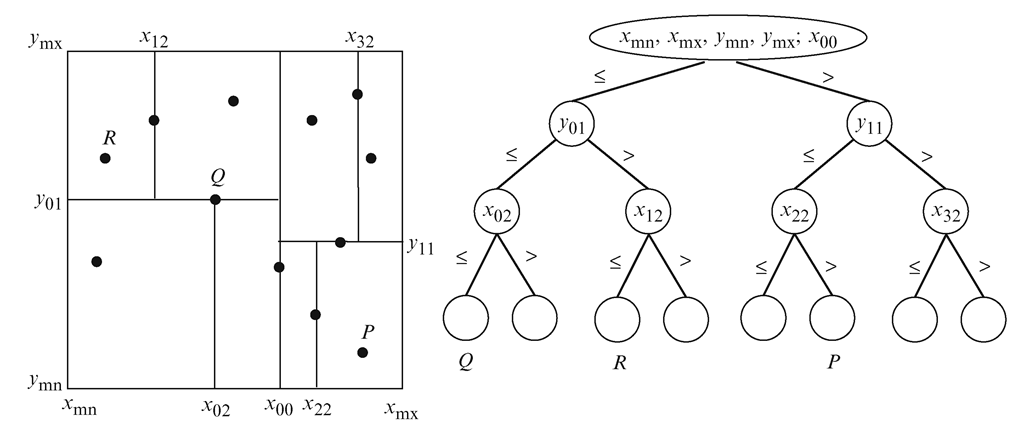
\includegraphics[width=\linewidth]{Figures/AABB}
	\caption{Esempio di albero di tipo AABB.}
	\label{AABB}
\end{figure}
%
\subsubsection{\textit{Arbitrarily Oriented Bounding Box}}
Il \ac{MBB} orientato arbitrariamente (\ac{AOBB}) è il rettangolo di delimitazione minimo, calcolato senza vincoli per quanto riguarda l'orientamento del risultato. Gli algoritmi del rettangolo di delimitazione minimo basati sul metodo dei calibri rotanti possono essere utilizzati per trovare l'area di delimitazione dell'area minima o del perimetro minimo di un poligono convesso bidimensionale in tempo lineare e di un punto bidimensionale impostato nel tempo impiegato costruire il suo scafo convesso seguito da un calcolo del tempo lineare. Un algoritmo di pinze rotanti tridimensionali può trovare il rettangolo di delimitazione orientato arbitrariamente sul volume minimo di un punto tridimensionale impostato in tempo cubo.
%
\subsubsection{\textit{Object Oriented Bounding Box}}
Nel caso in cui un oggetto abbia un proprio sistema di coordinate locale, può essere utile memorizzare un rettangolo di selezione relativo a questi assi, che non richiede alcuna trasformazione quando cambia l'orientazione dell'oggetto stesso.

\subsection{Intersezione tra Alberi AABB}
Per il rilevamento delle collisioni tra oggetti in due dimensioni, l'intersezione tra alberi di tipo \ac{AABB}, è l'algoritmo più veloce per determinare se le due entità di gioco si sovrappongono o meno, e in che parti. Nello specifico, ciò consiste nel controllare le posizioni delle \textit{i}-esime \ac{BB} nello spazio delle coordinate bidimensionali per vedere se si sovrappongono.

Il vincolo di allineamento dei rettangoli agli assi è presente per motivi di prestazioni, infatti, l'area di sovrapposizione tra due riquadri non ruotati può essere controllata solo con confronti logici. Mentre i riquadri ruotati richiedono ulteriori operazioni trigonometriche, che sono più lente da calcolare. Inoltre, se si hanno entità che possono ruotare, le dimensioni dei rettangoli e/o sotto-rettangoli dovranno modificarsi in modo da avvolgere ancora l'oggetto o si dovrà optare per un altro tipo di geometria di delimitazione, come le sfere (che sono invarianti alla rotazione).

Nel caso specifico, l'ombra dello pneumatico sarà rappresentata da un albero di tipo \ac{AABB} con una sola foglia. Ovvero si andrà a rappresentare lo pneumatico con una \ac{BB} avente lati uguali e rappresentanti il massimo ingombro che può avere nello spazio. Si andrà inoltre ad incrementare del 10\% ognuno di questi lati in modo da tenere conto dell'angolo di camber, che portrebbe portare i punti di campionamento del terreno fuori dall'ombra. La strada, contrariamente al pneumatico, verrà tenuta come riferimento assoluto. In altre parole, una volta effettuato la parsificazione del file \ac{RDF}, verrà calcolato l'albero di tipo \ac{AABB}. Lo pneumatico si muoverà all'interno della \textit{mesh} e la sua ombra verrà ricalcolata e intersecata con l'albero \ac{AABB} per ottenere tutti i triangoli in corrispondenza della stessa.

Volendo intersecare due semplici \ac{BB}, quali $A = \left[ \texttt{A.minX}, \texttt{A.maxX} ;  \texttt{A.minY}, \texttt{A.maxY} \right]$ e $B = \left[ \texttt{B.minX}, \texttt{B.maxX} ;  \texttt{B.minY}, \texttt{B.maxY} \right]$, verrà usata la seguente funzione.
\vspace{.8em}
\begin{pseudoc}
	function intersect(A,B) {
		return (A.minX <= B.maxX && A.maxX >= B.minX) &&
					 (A.minY <= B.maxY && A.maxY >= B.minY)
	}
\end{pseudoc}
\vspace{.5em}
\noindent
Volendo intersecare un albero di tipo \ac{AABB} e una semplice \ac{BB}, basterà ripetere a più step la funzione precedente lungo i rami dell'albero. Una volta arrivati a una o più foglia avremo tutti gli oggetti (o triangoli nel caso specifico) che sono posti in corrispondenza della \ac{BB} (od ombra dello pneumatico nel caso specifico). Questi triangoli verranno poi usati per determinare il piano strada locale e il punto di contatto virtuale dello pneumatico.

È imporatante notare che il metodo appena visto, presenta numerosi vantaggi.
\begin{itemize}
	\item Riduzione del numero di comparazioni da effettuare per ottenere l'intersezione \ac{BB}-albero \ac{AABB}. Infatti, la \textit{mesh} può contenere decine di migliaia di trangoli, il metodo presentato consente di ridurre logarirmicamente il numero di comparazioni necessarie per ottenere il risultato.
	\item Riduzione del numero di trangoli da processare per ottenere il piano strada locale e il punto di contatto virtuale dello pneumatico. Infatti, vengono solamente processati quelli posti in corrispondenza del'ombra dello pneumatico.
\end{itemize}
%
\section{Algoritmi Geometrici}
%
\subsection{Introduzione}
La geometria computazionale è la branca dell'informatica che studia le strutture dati e gli algoritmi efficienti per la soluzione di problemi di natura geometrica e la loro implementazione al calcolatore. Storicamente, è considerato uno dei campi più antichi del calcolo, anche se la geometria computazionale moderna è uno sviluppo recente. La ragione principale per lo sviluppo della geometria computazionale è stata dovuta ai progressi compiuti nella computer grafica, \ac{CAD}, \ac{CAM} e nella visualizzazione matematica. Ad oggi, le applicazioni della geometria computazionale si trovano nella robotica, nella progettazione di circuiti integrati, nella visione artificiale, in \ac{CAE} e nel \ac{GIS}. I rami principali della geometria computazionale sono:
\begin{itemize}
	\item \textit{Calcolo combinatorio} (o \textit{geometria algoritmica}), che si occupa di oggetti geometrici come entità discrete. Ad esempio, può essere utilizzato per determinare il poliedro o il poligono più piccolo che contiene tutti i punti forniti, o più formalmente, dato un insieme di punti, si deve determinare il più piccolo insieme convesso che li contenga tutti (problema dell'inviluppo convesso).
	\item \textit{Geometria di calcolo} numerica (o \ac{CAGD}), che si occupa principalmente di rappresentare oggetti del mondo reale in forme adatte per i calcoli informatici nei sistemi \ac{CAD} e \ac{CAM}. Questo ramo può essere visto come uno sviluppo della geometria descrittiva ed è spesso considerato un ramo della computer grafica o del \ac{CAD}. Entità importanti di questo ramo sono superfici e curve parametriche, come ad esempio le \textit{spline} e \textit{curve di Bézier}.
\end{itemize}

In questo capitolo tutti gli algoritmi che verranno utilizzati in seguito durante l'analisi geometrica dell'intersezione tra pneumatico e superficie stradale saranno trattati. Questi algoritmi sono la soluzione di alcuni semplici ma molto importanti problemi, che devono essere risolti in modo efficiente. In particolare le intersezioni tra:
\begin{itemize}
	\item punto e segmento (nel piano);
	\item punto e cerchio (nel piano);
	\item segmento e circonferenza (nel piano);
	\item piano e piano (nello spazio);
	\item piano e segmento (nello spazio);
	\item piano e raggio (nello spazio);
	\item piano e triangolo (nello spazio);
	\item raggio e triangolo (nello spazio);
\end{itemize}
saranno esaminati al fine di trovare la massima prestazione in termini di efficienza computazionale.
%
\subsection{Intersezione tra Entità Geometriche}
%
\subsubsection{Punto-Segmento}
Dato un punto $P = (x_p, y_p)$ e un segmento definito da due punti $A = (x_A, y_B)$ e $B = (x_B, y_B)$.

\begin{figure}[h!]
	\centering
	\begin{tikzpicture}
	\def\r{2};
	\coordinate (P) at (0.3,0.7);
	\coordinate (A) at (-2.0,0.0);
	\coordinate (B) at (+2.0,0.0);
	\draw[fill] (A) circle [radius=1pt] node[above] {$A$};
	\draw[fill] (B) circle [radius=1pt] node[above] {$B$};
	\draw[fill] (P) circle [radius=1pt] node[above] {$P$};
	\draw[thick](A) -- (B);
	\end{tikzpicture}
	\caption{Schema del problema di intersezione punto-segmento}
\end{figure}
\noindent
Per determinare se il punto $P$ è intermo al segmento si eseguiranno i seguenti step.
\begin{enumerate}
	\item Creazione di un vettore $\vv{AB}$ e di un vettore $\vv{AP}$.
	\item Calcolo il prodotto vettoriale  $\vv{P_1P_2} \times  \vv{PP_1}$, se il modulo del vettore risultante è nullo allora il punto $P$ appartiene al segmento considerato.
	\item Calcolo il prodotto scalare tra $\vv{AB}$ e $\vv{AP}$. Se è nullo allora il punto $P$ è coincidente a $A$, se è pari al modulo di $\vv{AB}$ allora il punto $P$ è coincidente a $B$, se è compreso tra 0 il modulo di $\vv{AB}$, allora il punto $P$ giace all'interno del segmento considerato.
\end{enumerate}
Il codice che esegue questo tipo di test è riportato in \figurename{ \ref{pointsegment}}

\begin{figure}[h!]
	\hfill
	\begin{subfigure}{.45\textwidth}
		\centering
		\begin{tikzpicture}
		\coordinate (P0) at (0.3,0.7);
		\coordinate (P3) at (-0.7,0);
		\coordinate (A) at (-2.0,0.0);
		\coordinate (B) at (+2.0,0.0);
		\draw[fill] (P0) circle [radius=1pt] node[above] {\texttt{0}};
		\draw[fill] (A) circle [radius=1pt] node[above] {\texttt{1}};
		\draw[fill] (B) circle [radius=1pt] node[above] {\texttt{2}};
		\draw[fill] (P3) circle [radius=1pt] node[above] {\texttt{3}};
		\draw[thick](A) -- (B);
		\end{tikzpicture}
		\caption{\textit{Output} di tipo \texttt{integer}}
	\end{subfigure}
	\hfill
	\begin{subfigure}{.45\textwidth}
		\centering
		\begin{tikzpicture}
		\coordinate (P0) at (0.3,0.7);
		\coordinate (P3) at (-0.7,0);
		\coordinate (A) at (-2.0,0.0);
		\coordinate (B) at (+2.0,0.0);
		\draw[fill] (P0) circle [radius=1pt] node[above] {\texttt{false}};
		\draw[fill] (A) circle [radius=1pt] node[above] {\texttt{true}};
		\draw[fill] (B) circle [radius=1pt] node[above] {\texttt{true}};
		\draw[fill] (P3) circle [radius=1pt] node[above] {\texttt{true}};
		\draw[thick](A) -- (B);
		\end{tikzpicture}
		\caption{\textit{Output} di tipo \texttt{bool}}
	\end{subfigure}
	\hfill
	\caption{Schemi per l'\textit{output} dell'intersezione punto-segmento.}
\end{figure}
\begin{figure}[h!]
	\hfill
	\begin{subfigure}[t]{.45\linewidth}
	\raggedright
	\textit{Output} di tipo \texttt{integer}\\
	\vspace{.5em}
	\begin{pseudoc}
	if ( AB.cross(AP) > epsilon )
		{ return 0; }
	KAP = AB.dot(AP);
	if ( KAP < -epsilon )
		{ return 0; }
	if ( abs(KAP) < epsilon  )
		{ return 1; }
	KAB = AB.dot(AB);
	if ( KAP > KAB )
		{ return 0; }
	if ( abs(KAP-KAB) < epsilon )
		{ return 2; }
	return 3;
	\end{pseudoc}
	\end{subfigure}
	\hfill
	\begin{subfigure}[t]{.45\textwidth}
	\raggedright
	\textit{Output} di tipo \texttt{bool}\\
	\vspace{.5em}
	\begin{pseudoc}
	if ( AB.cross(AP) > epsilon )
		{ return false; }
	KAP = AB.dot(AP);
	if ( KAP < -epsilon )
		{ return false; };
	if ( abs(KAP) < epsilon )
		{ return true; }
	KAB = AB.dot(AB);
	if ( KAP > KAB ) 
		{ return false; }
	if ( abs(KAP-KAB) < epsilon )
		{ return true; }
	return true;
	\end{pseudoc}
	\end{subfigure}
	\hfill
	\caption{Schema del codice per l'intersezione punto-segmento.}
	\label{pointsegment}
\end{figure}
%
\subsubsection{Punto-Cerchio}
Data una circonferenza con centro $C = (x_c, y_c)$ e raggio $r$, il problema consiste nel trovare se un punto generico $P = (x_p, y_p)$ è locato all'interno, all'esterno o sulla circonferenza.
\begin{figure}[h]
	\centering
	\begin{tikzpicture}
	\def\r{2};
	\coordinate (C) at (0,0) node[above left] {$C$};
	\draw[thick, fill=gray!10](C) circle (\r);
	\coordinate (P) at (-0.5,-1.5);
	\draw[fill] (C) circle [radius=1pt];
	\draw[fill] (P) circle [radius=1pt];
	\draw(C) -- (P)  node[above left] {$P$} node[pos=0.5, right] {$d$};
	\draw(C) -- ({sqrt(\r)},{sqrt(\r)}) node[pos=0.4, above] {$r$};
	\end{tikzpicture}
	\caption{Schema del problema di intersezione punto-cerchio.}
\end{figure}
La soluzione al problema è semplice: la distanza tra il centro del cerchio $C$ e il punto $P$ è data dal teorema di Pitagora. In particolare:
\begin{equation}
	d=\sqrt{(x_p-x_c)^2 + (y_p-y_c)^2}
\end{equation}
il punto $P$ è dunque interno alla circonferenza se $d<r$, appartiene alla circonferenza se $d=r$ ed esterno alla circonferenza se $d>r$. In maniera analoga ma più efficace da punto di vista computazionale si può confrontare $d^2$ con $r^2$. Il punto $P$ è dunque interno alla circonferenza se $d^2<r^2$,  appartiene alla circonferenza se $d^2=r^2$ ed esterno alla circonferenza se $d^2>r^2$. Pertanto, il confronto finale sarà tra il numero $(x_p-x_c)^2+(y_p-y_c)^2 $ e $r^2$.

\noindent
Gli \textit{inputs} dell'algoritmo per l'intersezione punto-cerchio sono:
\begin{itemize}
	\item il centro della circonferenza $C = (x_c, y_c)$;
	\item il raggio della circonferenza $r$;
	\item il punto generico da analizzare $P=(x_p, y_p)$.
\end{itemize}
L'\textit{output} può essere un intero il cui valore può essere:
\begin{itemize}
	\item \texttt{0} se il punto è esterno;
	\item \texttt{1} se il punto è interno;
	\item \texttt{2} se il punto appartiene alla circonferenza.
\end{itemize}
Il valore in \textit{output} può essere anche una variabile booleana il cui valore è:
\begin{itemize}
	\item \texttt{false} se il punto è esterno;
	\item \texttt{true} se il punto è interno o appartiene alla circonferenza.
\end{itemize}
%
\begin{figure}[h]
\hfill
	\begin{subfigure}{.45\textwidth}
	\centering
	\begin{tikzpicture}
	\def\r{2};
	\coordinate (C) at (0,0);
	\draw[thick, fill=gray!10](C) circle (\r);
	\draw[fill] (0,-0.5) circle [radius=1pt] node[above left] {\texttt{1}};
	\draw[fill] (-\r,0) circle [radius=1pt] node[above left] {\texttt{2}};
	\draw[fill] (3,0) circle [radius=1pt] node[above left] {\texttt{0}};
	\end{tikzpicture}
	\caption{\textit{Output} di tipo \texttt{integer}}
\end{subfigure}
\hfill
\begin{subfigure}{.45\textwidth}
	\centering
	\begin{tikzpicture}
	\def\r{2};
	\coordinate (C) at (0,0);
	\draw[thick, fill=gray!10](C) circle (\r);
	\draw[fill] (0,-0.5) circle [radius=1pt] node[above left] {\texttt{true}};
	\draw[fill] (-\r,0) circle [radius=1pt] node[above left] {\texttt{true}};
	\draw[fill] (3,0) circle [radius=1pt] node[above] {\texttt{false}};
	\end{tikzpicture}
	\caption{\textit{Output} di tipo \texttt{bool}}
\end{subfigure}
\hfill
\caption{Schemi per l'\textit{output} dell'intersezione punto-cerchio.}
\end{figure}
\begin{figure}[h]
\hfill
	\begin{subfigure}[t]{.475\linewidth}
	\raggedright
	\textit{Output} di tipo \texttt{integer}\\
	\vspace{.5em}
	\begin{pseudoc}
	d = (x_p-x_c)^2 + (y_p-y_c)^2;
	if ( d > r^2 ){ return  0; }
	else if ( d < r^2 ){ return 1; }
	else { return 2; }
	\end{pseudoc}
	\end{subfigure}
\hfill
	\begin{subfigure}[t]{.475\textwidth}
	\raggedright
	\textit{Output} di tipo \texttt{bool}\\
	\vspace{1em}
	\begin{pseudoc}
	d = (x_p-x_c)^2 + (y_p-y_c)^2;
	if ( d > r^2 ){ return  true; }
	else { return false; }
	\end{pseudoc}	
	\end{subfigure}
\hfill
\caption{Schemi del codice per l'intersezione punto-cerchio.}
\label{Pointcircle}
\end{figure}
%
\subsubsection{Segmento-Circonferenza}
Per l'intersezione di un segmento, avente punto iniziale e finale rispettivamente $P_0$ e $P_1$, con una circonferenza, avente centro $C=(x_c,y_c)$, è necessario prima di tutto riscrivere le equazione di entrambe le entità come:
\begin{equation}
ax+by=c
\label{eqretta}
\end{equation}
per il segemento e:
\begin{equation}
(x-x_c)^2 + (y-y_c)^2 = r^2
\end{equation}
per la circonferenza. Assumendo che il centro $C$ sia posto sull'origine, la precedente equazione si può semplificare come:
\begin{equation}
x^2 + y^2 = r^2
\label{eqcircle}
\end{equation}
\begin{figure}[h]
	\centering
	\begin{tikzpicture}
	\def\r{2};
	\coordinate (C) at (0,0);
	\coordinate (P0) at (-4,-1);
	\coordinate (P1) at (4,-1);
	\draw[thick, fill=gray!10](C) circle (\r);
	\draw[fill] (C) circle [radius=1pt];
	\draw[fill] (P0) circle [radius=1pt];
	\draw[fill] (P1) circle [radius=1pt];
	\draw[thick](P0) -- (P1) node[above] {$P_1$} node[pos=0, above] {$P_0$};
	\draw(C) -- ({sqrt(\r)},{sqrt(\r)}) node[pos=0.4, above] {$r$};
	\draw[fill] ({-sqrt(3)/2*\r},{-0.5*\r}) circle [radius=1pt] node[below left] {$(x_1,y_1)$};
	\draw[fill] ({sqrt(3)/2*\r},{-0.5*\r}) circle [radius=1pt] node[below right] {$(x_2,y_2)$};
	\end{tikzpicture}
	\caption{Schema del problema di intersezione punto-circonferenza.}
\end{figure}
Per trovere i termini $a$, $b$ e $c$ del segmento è necessario calcolare la direzione del segmento come differenza tra il punto finale e iniziale del segmento:
\begin{equation}
\vec{d} = P_1 - P_0 
\end{equation}
È neccerio anche trovare il vettore tra l'origine e il punto $P_1$:
\begin{equation}
\vec{P}_{O1} = P_1 - O
\end{equation}
I termini $a$, $b$ e $c$ del segmento saranno quini pari a:
\begin{equation}
\begin{aligned}
	\begin{split}
		a =& \vec{d} \cdot \vec{d} \\
		b =& 2 (\vec{d} \cdot \vec{P}_{O1}) \\
		c =& \vec{P}_{O1} \cdot \vec{P}_{O1} - r^2
	\end{split}
\end{aligned}
\end{equation}
Risolvere l'equazione \ref{eqretta} per $x$ o $y$ è ora molto semplice. Basta infatti sostituirla nell'equazione \ref{eqcircle} per ottere le soluzioni $(x_1, y_1)$ e $(x_2, y_2)$ con:
\begin{equation}
x_{1/2} = \frac{ac \pm b \sqrt{r^2 (a^2 + b^2)-c^2}}{a ^ 2 + b ^ 2}
\end{equation}
oppure:
\begin{equation}
y_{1/2} = \frac{bc \mp a \sqrt{r^2 (a^2 + b^2)-c^2}}{a ^ 2 + b ^ 2}
\end{equation}
Se $r^2 (a^2 + b^2)-c^2 \geq 0$ vale come una disuguaglianza stretta, esistono due punti di intersezione.\\
Se invece vale $r^2 (a^2 + b^2)-c^2 = 0$, allora esiste solo un punto di intersezione e la linea è tangente alla circonferenza. Se la disuguaglianza debole non regge, la linea non interseca la circonferenza.\\
\noindent
Dal punto di vista del codice l'\textit{output} può essere un intero il cui valore può essere:
\begin{itemize}
	\item \texttt{0} se la linea non interseca la circonferenza;
	\item \texttt{1} se la linea interseca la circonferenza in un solo punto, ovvero è tangente;
	\item \texttt{2} se la linea interseca la circonferenza in due punti.
\end{itemize}

\begin{figure}[h]
	\hfill
	\begin{subfigure}{.3\textwidth}
		\centering
		\begin{tikzpicture}
		\def\r{1.5};
		\coordinate (C) at (0,0);
		\coordinate (P0) at (-2,-1.75);
		\coordinate (P1) at (2,-1.75);
		\draw[thick, fill=gray!10](C) circle (\r);
		\draw(C) node {\texttt{0}};
		\draw[fill] (P0) circle [radius=1pt];
		\draw[fill] (P1) circle [radius=1pt];
		\draw[thick](P0) -- (P1) node[above] {$P_1$} node[pos=0, above] {$P_0$};
		\end{tikzpicture}
	\end{subfigure}
	\hfill
	\begin{subfigure}{.3\textwidth}
		\centering
		\begin{tikzpicture}
		\def\r{1.5};
		\coordinate (C) at (0,0);
		\coordinate (P0) at (-2,-1.5);
		\coordinate (P1) at (2,-1.5);
		\draw[thick, fill=gray!10](C) circle (\r);
		\draw(C) node {\texttt{1}};
		\draw[fill] (P0) circle [radius=1pt];
		\draw[fill] (P1) circle [radius=1pt];
		\draw[thick](P0) -- (P1) node[above] {$P_1$} node[pos=0, above] {$P_0$};
		\draw[fill] (0,-\r) circle [radius=1pt];
		\end{tikzpicture}
	\end{subfigure}
	\hfill
	\begin{subfigure}{.3\textwidth}
		\centering
		\begin{tikzpicture}
		\def\r{1.5};
		\coordinate (C) at (0,0);
		\coordinate (P0) at (-2,-0.75);
		\coordinate (P1) at (2,-0.75);
		\draw[thick, fill=gray!10](C) circle (\r);
		\draw(C) node {\texttt{2}};
		\draw[fill] (P0) circle [radius=1pt];
		\draw[fill] (P1) circle [radius=1pt];
		\draw[thick](P0) -- (P1) node[above] {$P_1$} node[pos=0, above] {$P_0$};
		\draw[fill] ({-sqrt(3)/2*\r},{-0.5*\r}) circle [radius=1pt];
		\draw[fill] ({sqrt(3)/2*\r},{-0.5*\r}) circle [radius=1pt];
		\end{tikzpicture}
	\end{subfigure}
	\hfill
	\caption{Schemi per l'\textit{output} dell'intersezione segmento-cerchio.}
\end{figure}
\begin{figure}[htbp]
	\centering
	\begin{subfigure}{.65\linewidth}
	\begin{pseudoc}
	a = d $\cdot$ d;
	b = 2 * (d $\cdot$ P_O1);
	c = P_O1 $\cdot$ P_O1 - r^2;
	discriminant = r^2 * (a^2 + b^2) - c^2;
	if ( a <= epsilon || discriminant < 0.0 ) {
		IntPt_1 = (quiteNaN, quiteNaN);
		IntPt_2 = (quiteNaN, quiteNaN);
		return 0;
	} else if ( abs(discriminant) < epsilon ) {
		t = - b / (2 * a);
		IntPt_1 = P_1 + t * d;
		IntPt_2 = (quiteNaN, quiteNaN);
		return 1;
	} else {
		t = (-b + sqrt(discriminant)) / (2 * a);
		IntPt_1 = P_1 + t * d;
		t = (-b - sqrt(discriminant)) / (2 * a);
		IntPt_2 = P_1 + t * d;
		return 2;
	}
	\end{pseudoc}
	\end{subfigure}
	\caption{Schema per del codice per l'intersezione segmento-cerchio.}
\end{figure}
%
\subsubsection{Piano-Piano}
Nello spazio delle coordinate tridimensionali, due piani $P_1$ e $P_2$ o sono paralleli o si intersecano creando una singola retta $L$. Sia $P_i$ con $i = 1,2$ descritto da un punto $V_i$ e un vettore normale $\vec{n}_i$. L'equazione implicita del piano sarà dunque:
\begin{equation}
\vec{n}_i \cdot P + d_i = 0
\end{equation}
dove $P = (x, y, z)$. I piani $P_1$ e $P_2$ sono paralleli ogni volta che i loro normali vettori $\vec{n}_1$ e $\vec{n}_2$ sono paralleli. Questo equivale alla condizione che $\vec{n}_1 \times \vec{n}_2 = 0$. Quando i piani non sono paralleli, $\vec{u} = \vec{n}_1 \times \vec{n}_2$ è il vettore di direzione della linea di intersezione $L$. Si noti che $\vec{u}$ è perpendicolare sia a $\vec{n}_1$ che a $\vec{n}_2$, e quindi è parallelo a entrambi i piani.

\begin{figure}
	\centering
	\tdplotsetmaincoords{70}{110}
	\begin{tikzpicture}[tdplot_main_coords,font=\sffamily]
	\draw[-latex] (0,0,0) -- (4,0,0) node[left] {$x$};
	\draw[-latex] (0,0,0) -- (0,4,0) node[below] {$y$};
	\draw[-latex] (0,0,0) -- (0,0,4) node[left] {$z$};
	\tdplotsetrotatedcoords{45}{0}{0}
	\begin{scope}[tdplot_rotated_coords]
	\draw[fill=gray!10,opacity=0.6] (-3,0,-3) -- (-3,0,3) -- (3,0,3) -- (3,0,-3) -- cycle;
	\end{scope}
	\tdplotsetrotatedcoords{90}{45}{0}
	\begin{scope}[tdplot_rotated_coords]
	\draw[fill=gray!10,opacity=0.5] (-3,-3,0) -- (-3,3,0) -- (3,3,0) -- (3,-3,0) -- cycle;
	\draw[thick](-3,{3/sqrt(2)},0) coordinate(x) --(3,{-3/sqrt(2)},0);
	\end{scope}
	\node[anchor=south east,align=center] (line) at (3,-1.5,3.5) {$L$};
	\draw[-latex] (line) to[out=0,in=135] (x);
	\end{tikzpicture}
	\caption{Schemi del problema di intersezione piano-piano.}
\end{figure}

Dopo aver calcolato $\vec{n}_1 \times \vec{n}_2$, per determinare univocamente la linea di intersezione, è necessario trovare un punto di essa. Cioè, un punto $P_0 = (x_0, y_0, z_0)$ che si trova in entrambi i piani. Si può trovare una soluzione comune delle equazioni implicite per $P_1$ e $P_2$. Ma ci sono solo due equazioni nelle tre incognite poiché il punto $P_0$ può trovarsi ovunque sulla linea monodimensionale $L$. Quindi è necessario aggiungere un altro vincolo da risolvere per un $P_0$ specifico. Esistono diversi modi per farlo, il più semplice è attraverso l'aggiunta dei un terzo piano $P_3$ avente equazione implicita $\vec{n}_3 \cdot P = 0$ dove $\vec{n}_3 = \vec{n}_1 \times \vec{n}_2$ e $d_3 = 0$ (ovvero passa attraverso l'origine). Questo metodo è funzionante poiché: 
\begin{itemize}
	\item $L$ è perpendicolare a $P_3$ e quindi lo interseca;
	\item i vettori $\vec{n}_1$, $\vec{n}_2$ e $\vec{n}_3$ sono linearmente indipendenti.
\end{itemize}
Pertanto i piani $P_1$, $P_2$ e $P_3$ si intersecano in un unico punto $P_0$ che deve trovarsi su $L$. 

\begin{figure}
	\centering
	\tdplotsetmaincoords{70}{110}
	\begin{tikzpicture}[tdplot_main_coords]
	\draw[-latex] (0,0,0) -- (4,0,0) node[left] {$x$};
	\draw[-latex] (0,0,0) -- (0,4,0) node[below] {$y$};
	\draw[-latex] (0,0,0) -- (0,0,4) node[left] {$z$};
	\draw[fill=gray!10,opacity=0.6] (-3,0,-3) -- (-3,0,3) -- (3,0,3) -- (3,0,-3) -- cycle;
	\draw[fill=gray!10,opacity=0.5] (-3,-3,0) -- (-3,3,0) -- (3,3,0) -- (3,-3,0) -- cycle;
	\draw[dashed] (-3,0,0)--(3,0,0);
	\draw[-stealth,thick] (0,0,0) -- (2,0,0);
	\draw[-stealth,thick] (0,0,0) -- (0,2,0) node[above] {$\vec{n}_1$};
	\draw[-stealth,thick] (0,0,0) -- (0,0,2) node[left] {$\vec{n}_2$};
	\draw(2,.1,0) node[right] {$\vec{n}_3$};
	\end{tikzpicture}
	\caption{Vettori dei piani $P_1$, $P_2$ e della retta $L$.}
\end{figure}

Nello specifico, la formula per l'intersezione di tre piani è:
\begin{equation}
P_0 =  \frac{-d_1(\vec{n}_2 \times \vec{n}_3) - d_2(\vec{n}_3 \times \vec{n}_1) - d_3(\vec{n}_1 \times \vec{n}_2)}{\vec{n}_1 \cdot (\vec{n}_2 \times \vec{n}_3)}
\end{equation}
e ponendo $d_3 = 0$ per $P_3$, si otteniene:
\begin{equation}
P_0 =  \frac{-d_1(\vec{n}_2 \times \vec{n}_3) - d_2(\vec{n}_3 \times \vec{n}_1)}{\vec{n}_1 \cdot (\vec{n}_2 \times \vec{n}_3)}
=
\frac{(d_2\vec{n}_1 - d_1\vec{n}_2) \times \vec{n}_3}{(\vec{n}_1 \times \vec{n}_2) \cdot \vec{n}_3}
=
\frac{(d_2\vec{n}_1 - d_1\vec{n}_2) \times \vec{u}}{|\vec{u}|^2}
\end{equation}
e l'equazione parametrica per la retta $L$ sarà:
\begin{equation}
L(s) =
\frac{(d_2\vec{n}_1 - d_1\vec{n}_2) \times \vec{u}}{|\vec{u}|^2}+s\vec{u}
\end{equation}
dove $\vec{u}=\vec{n}_1 \times \vec{n}_2$.

\begin{figure}[htbp]
	\centering
	\begin{subfigure}{.65\linewidth}
		\begin{pseudoc}
	u = n_1 $\times$ n_2;
	if ( u.norm() > epsilon ) {
		d_1 = - V_1 $\cdot$ n_1;
		d_2 = - V_2 $\cdot$ n_2;
		u_1 = d_1 * n_1;
		u_2 = - d_2 * n_2;
		P_0 = (u1 + u2) $\times$ u / (u $\cdot$ u);
		return true;
	} else {
		return false;
	}
		\end{pseudoc}
	\end{subfigure}
	\caption{Schema per del codice per l'intersezione piano-piano.}
\end{figure}
%
\subsubsection{Piano-Segmento e Piano-Raggio}
Nello spazio delle coordinate tridimensionali, una linea $L$ può essere o parallela a un piano $P$ o può intersecarlo in un singolo punto. Sia $L$ data dall'equazione parametrica:
\begin{equation}
P(t) = P_0 + t(P_1-P_0) = P_0 + t\vec{u}
\end{equation}
mentre il piano $P$ sia dato da un punto $V_0$ appartenente ad esso e da un vettore normale $\vec{n} = (a,b,c)$. Per prima cosa è necessario controllare se $L$ è parallelo a $P$ verificando se $\vec{n}\cdot\vec{u} = 0$, il che significa che il vettore di direzione della linea $\vec{u}$ è perpendicolare al piano normale $\vec{n}$. Se questo è vero, allora $L$ e $P$ sono paralleli e non si intersecano, oppure $L$ giace totalmente nel piano $P$. Disgiunzione o coincidenza possono essere determinate testando se in $P$ esiste un punto specifico di $L$, per esempio $P_0$, ovvero se soddisfa l'equazione di linea implicita:
\begin{equation}
\vec{n} \cdot (P_0-V_0) = 0
\end{equation}
Se la linea e il piano non sono paralleli, allora $L$ e $P$ si intersecano in un unico punto $P(t_I)$. Nel punto di intersezione, il vettore $P(t)-V_0 = \vec{w} + t\vec{u}$ è perpendicolare a $\vec{n}$, dove $\vec{w} = P_0-V_0$. Ciò equivale alla condizione del prodotto scalare:
\begin{equation}
\vec{n} \cdot (\vec{w}+t\vec{u}) = 0
\end{equation}
Risolvendo si ottiene:
\begin{equation}
t_I = -\frac{\vec{n}\cdot\vec{w}}{\vec{n}\cdot\vec{u}}
=
-\frac{\vec{n}\cdot(V_0-P_0)}{\vec{n}\cdot(P_1-P_0)}
\end{equation}
Se la linea $L$ è un segmento finito da $P_0$ a $P_1$, è sufficiente verificare che $0 \leq t_I \leq 1$ per verificare che vi sia un'intersezione tra il segmento e il piano. Per raggio, c'è invece un'intersezione con il piano quando $t_I \geq 0$.

\begin{figure}[htbp]
	\centering
	\tdplotsetmaincoords{70}{110}
	\begin{tikzpicture}[tdplot_main_coords]
	\draw[-latex] (0,0,0) -- (4,0,0) node[left] {$x$};
	\draw[-latex] (0,0,0) -- (0,4,0) node[below] {$y$};
	\draw[-latex] (0,0,0) -- (0,0,4) node[left] {$z$};
	
	\draw[fill=gray!10,opacity=0.5] (-3,-3,0) -- (-3,3,0) -- (3,3,0) -- (3,-3,0) -- cycle;
	\draw[-stealth,thick] (0,-0.75,3.25) node[above] {$P_0$} -- (0,1.25,1.25) node[above right] {$P_1$};
	\draw (0,-0.5,2.25) node[below left] {$\vec{w}$};
	\draw (0,0.25,2.25) node[above right] {$\vec{u}$};
	\draw[-stealth,thick] (0,0,0) -- (0,-0.75,3.25);
	\draw[dashed] (0,1.25,1.25) -- (0,2.5,0);
	\draw[fill] (0,2.5,0) circle [radius=1pt];
	\draw (0,2.5,0) node[below left] {$P(t_I)$};
	\draw (0,2,0.5) node[right] {$P(t)$};
	\draw[fill] (0,2,.5) circle [radius=1pt];
	\draw[-stealth,thick] (1,-2,0) -- (1,-2,2) node[left] {$\vec{n}$};
	\end{tikzpicture}
	\caption{Vettori dei piani $P_1$, $P_2$ e della retta $L$.}
\end{figure}
\begin{figure}[htbp]
	\centering
	\begin{subfigure}{.5\linewidth}
		\begin{pseudoc}
	u = P_1 - P_0;
	t = n $\cdot$ (V_0 - P_0) / (u $\cdot$ n);
	if ( t >= 0 && t <= 1 ) {
		P_tI = P_0 + u * t;
		return true;
	} else {
		return false;
	}
		\end{pseudoc}
	\end{subfigure}
	\caption{Schema per del codice per l'intersezione piano-segmento.}
\end{figure}
%
\subsubsection{Piano-Triangolo}
Per risolvere l'intersezione piano triangolo bastaunsare la soluzione precedentemente trovata per il problame dell'intersezione tra piano e segmento. Nello specifico, basta trattare i lati del triangolo come tre segmenti distinti e per ognuno di esso applicare la funzione per l'intersezione piano-segmento. Vi saranno tre possibili soluzioni:
\begin{itemize}
	\item il triangolo non viene intersecato dal piano;
	\item il triangolo viene intersecato dal piano in uno dei suoi tre vertici;
	\item il triangolo viene intersecato dal piano, formando quindi due punti d'intersezione nel suo perimetro.
\end{itemize}

\begin{figure}[htbp]
	\centering
	\begin{subfigure}{.7\linewidth}
		\begin{pseudoc}
	if ( intersectSegmentPlane( n, V_0, 1, IntPt_1 ))
	{ IntPts.push_back(IntPt1); }
	if ( intersectSegmentPlane( n, V_0, 2, IntPt2 ))
	{ IntPts.push_back(IntPt2); }
	if ( intersectSegmentPlane( n, V_0, 3, IntPt3 ))
	{ IntPts.push_back(IntPt3); }
	if ( IntPts.size() == 2 ) 
	{ return true; }
	else if ( IntPts.size() == 0 ) 
	{ return false; }
	else 
	{ return false; }
		\end{pseudoc}
	\end{subfigure}
	\caption{Schema per del codice per l'intersezione piano-triangolo.}
\end{figure}
%
\subsubsection{Raggio-Triangolo}
Dato un triangolo avente vertici $(A,B,C)$ e un raggio $R$ con origine $R_O$ e direzione $\vec{R}_D$, il problema consiste nel capire se il raggio colpisce o meno il triangolo e, in tal caso, trovare il punto di intersezione $P$.
%
\begin{figure}[htbp]
	\centering
	\begin{tikzpicture}
	\coordinate [label=left:$A$] (A) at (-1,-0.5);
	\coordinate [label=above:$B$] (B) at (1,1);
	\coordinate [label=right:$C$] (C) at (2.2,-1);
	\draw[fill=gray!10] (A) -- (B) -- (C) -- (A);
	\def\xp{0.4};
	\def\yp{-0.2};
	\def\xd{-1};
	\def\yd{1};
	\def\mag{1.7};
	\coordinate [label=above right:$P$] (P) at (\xp,\yp);
	\coordinate [label={[shift={(0.1,0.1)}]$\vec{R}_D$}] (RD) at (\xp+\xd,\yp+\yd);
	\coordinate [label=above:$R_O$] (RO) at (\xp+\xd*\mag,\yp+\yd*\mag);
	\draw[fill] (P) circle [radius=1pt];
	\draw[fill] (RO) circle [radius=1pt];
	\draw[-stealth] (RO) -- (RD);
	\draw[dashed] (RD) -- (P);
	\end{tikzpicture}
	\caption{Schema del problema di intersezione raggio-triangolo.}
\end{figure}
%
Negli ultimi decenni, sono stati proposti numerosi algoritmi per risolvere questo problema, esistono quindi diverse soluzioni al problema di intersezione raggio-triangolo. Tre degli algoritmi più importanti sono:
\begin{itemize}
	\item l'agoritmo di \textit{Badouel};
	\item l'agoritmo di \textit{Segura};
	\item l'agoritmo di \textit{M\"oller} e \textit{Trumbore}.
\end{itemize}
\noindent
Come \citeauthor{RayTriangle} afferma in \cite{RayTriangle}, l'algoritmo di M\"oller-Trumbore's è il più veloce quando il piano normale e/o il piano di proiezione non sono stati precedentemente memorizzati, come nel caso specifico di questa tesi.

La teoria alla base di questo algoritmo è spiegata estensivamente in \cite{Moller}. In particolare, l'algoritmo sfrutta la parametrizzazione di $P$, il punto di intersezione, in termini delle coordinate baricentriche, ovvero:
\begin{equation}
	P = wA + uB + vC
\end{equation}
Dato che $w = 1-u-v$, si può quindi scrivere:
\begin{equation}
	P = (1-u-v)A + uB + vC
\end{equation}
e sviluppando si ottiene:
\begin{equation}
	P = A-uA-vA+uB+vC = A+u(B-A)+v(C-A)
	\label{eq1}
\end{equation}
Si noti che $(B-A)$ e $(C-A)$ sono i bordi $AB$ e $AC$ del triangolo $ABC$. L'intersezione $P$ può anche essere scritta usando l'equazione parametrica del raggio:
\begin{equation}
	P = R_O + t\vec{R}_D
	\label{eq2}
\end{equation}
dove $t$ è la distanza dall'origine del raggio all'intersezione $P$. Sostituendo $P$ nell'equazione \ref{eq1} con l'equazione del raggio si ottiene:
\begin{equation}
	\begin{split}
	\begin{aligned}
		R_O + t\vec{R}_D =& A+u(B-A)+v(C-A)\\
		O - A =& -tD+u(B-A)+v(C-A)
	\end{aligned}
	\end{split}
	\label{eq3}
\end{equation}
Sul membro a sinistra si hanno le tre incognite $(t,u,v)$ moltiplicate per tre termini noti $(B-A, C-A, D)$. Si può riorganizzare questi termini e presentare l'equazione \ref{eq3} usando la seguente notazione:
\begin{equation}
	\begin{bmatrix}
	-D & (B-A) & (C-A)
	\end{bmatrix}
	\begin{bmatrix}
	t \\
	u \\
	v
	\end{bmatrix} = R_O - A
	\label{eq4}
\end{equation}
Si immagini ora di avere un punto $P$ all'interno del triangolo. Se si trasforma il triangolo in qualche modo (ad esempio traslandolo, ruotandolo o scalandolo), le coordinate del punto $P$ espresse nel sistema di coordinate cartesiane tridimensionali $(x,y,z)$ cambieranno. D'altra parte, se si esprime la posizione di $P$ usando le coordinate baricentriche, le trasformazioni applicate al triangolo non influenzeranno le coordinate baricentriche del punto di intersezione. Se il triangolo viene ruotato, ridimensionato, allungato o traslato, le coordinate $(u,v)$ che definiscono la posizione di $P$ rispetto ai vertici $(A,B,C)$ non cambieranno. L'algoritmo di M\"oller-Trumbore sfrutta proprio questa proprietà. Infatti, ciò che gli autori hanno fatto è definire un nuovo sistema di coordinate in cui le coordinate di $P$ non sono definite in termini di $(x,y,z)$ ma in termini di $(u,v)$. La somma tra le coordinate baricentriche non può essere maggiore di 1 ($u + v \leq 1$), esprimono infatti le coordinate dei punti definiti all'interno di un triangolo unitario. Ovvero un triangolo definito nello spazio $(u,v)$ dai vertici $(0,0)$, $(1,0)$, $(0,1)$.

\begin{figure}[htbp]
	\centering
	\hfill
	\begin{subfigure}[t]{.45\linewidth}
		\begin{tikzpicture}
		\coordinate (O) at (0,0,0);
		\def\axisl{3}
		\draw[-stealth] (O) -- (\axisl,0,0) node[below]{$x$};
		\draw[-stealth] (O) -- ({sqrt(\axisl)},{sqrt(\axisl)},0) node[above]{$y$};
		\draw[-stealth] (O) -- (0,\axisl,0) node[left]{$z$};
		\coordinate [label=below:$C$] (V1) at ({\axisl/1.5},0.5,0);
		\coordinate [label=above:$B$] (V2) at ({sqrt(\axisl)/1.5},{3.3/1.8},0);
		\coordinate [label={[shift={(-0.15,0)}]$A$}] (V3) at (0.3,0.6,0);
		\draw[fill=gray!10] (V1) -- (V2) -- (V3) -- (V1);
		
		\def\xp{1};
		\def\yp{1};
		\def\xd{-1};
		\def\yd{0.8};
		\def\mag{1.7};
		\coordinate [label=above:$P$] (P) at (\xp,\yp);
		\coordinate [label={[shift={(-0.3,-0.5)}]$\vec{R}_D$}] (RD) at (\xp+\xd*1.1,\yp+\yd*1.1);
		\coordinate [label=above:$R_O$] (RO) at (\xp+\xd*\mag*1.1,\yp+\yd*\mag*1.1);
		\draw[fill] (P) circle [radius=1pt];
		\draw[fill] (RO) circle [radius=1pt];
		\draw[-stealth] (RO) -- (RD);
		\draw[dashed] (RD) -- (P);
		\end{tikzpicture}
	\end{subfigure}
	\hfill
	\begin{subfigure}[t]{.45\linewidth}
		\begin{tikzpicture}
		\coordinate (O) at (0,0,0);
		\def\axisl{3}
		\draw[-stealth] (O) -- (\axisl,0,0) node[below]{$\alpha$};
		\draw[-stealth] (O) -- ({sqrt(\axisl)},{sqrt(\axisl)},0) node[above]{$\beta$};
		\draw[-stealth] (O) -- (0,\axisl,0) node[left]{$\gamma$};
		\coordinate [label={[below,font=\tiny]:$1$}] (V1) at ({\axisl/1.5},0,0);
		\coordinate [label={[shift={(-0.1,0.0)},font=\tiny]:$1$}] (V2) at ({sqrt(\axisl)/1.5},{sqrt(\axisl)/1.5},0);
		\coordinate (V3) at (0,0,0);
		\draw[fill=gray!10] (V1) -- (V2) -- (V3) -- (V1);
				
		\def\xp{0.7};
		\def\yp{0.35};
		\def\xd{0};
		\def\yd{1};
		\def\mag{1.7};
		\coordinate [label=right:$P$] (P) at (\xp,\yp);
		\coordinate [label={[shift={(-0.35,-0.15)}]$\vec{R}_D$}] (RD) at (\xp+\xd,\yp+\yd);
		\coordinate [label=above:$R_O$] (RO) at (\xp+\xd*\mag,\yp+\yd*\mag);
		\draw[fill] (P) circle [radius=1pt];
		\draw[fill] (RO) circle [radius=1pt];
		\draw[-stealth] (RO) -- (RD);
		\draw[dashed] (RD) -- (P);
		\end{tikzpicture}
	\end{subfigure}
	\hfill
	\caption{Cambiamento di coordinate nell'algoritmo di M\"oller-Trumbore.}
\end{figure}

Geometricamente, si è appena chiarito il significato di $u$ e $v$. Si consideri ora l'elemento $t$. Esso è il terzo asse del sistema di coordinate $u$ e $v$ appena introdotto. Si sà inoltre che $t$ esprime la distanza dall'origine del raggio a $P$, il punto di intersezione, si è quindi creato un sistema di coordinate che consentirà di esprimere univocamente la posizione del punto d'intersezione $P$ in termini di coordinate baricentriche e distanza dall'origine del raggio a quel punto sul triangolo.

M\"oller e Trumbore spiegano che la prima parte dell'equazione \ref{eq4} (il termine $O-A$) può essere vista come una trasformazione che sposta il triangolo dalla sua posizione spaziale mondiale originale all'origine (il primo vertice del triangolo coincide con l'origine). L'altro lato dell'equazione ha l'effetto di trasformare il punto di intersezione dallo spazio $(x,y,z)$ nello spazio $(t,u,v)$ come spiegato precedentemente.

Per risolvere l'equazione \ref{eq4}, M\"oller e Trumbore hanno usato una tecnica conosciuta in matematica come regola di Cramer. La regola di Cramer fornisce la soluzione a un sistema di equazioni lineari mediante il determinante. La regola afferma che se la moltiplicazione di una matrice $M$ per un vettore colonna $X$ è uguale a un vettore colonna $C$, allora è possibile trovare $X_i$ (l'$i$-esimo elemento del vettore colonna $X$) dividendo il determinante di $M_i$ per il determinante di $M$. Dove $M_i$ è la matrice formata sostituendo la sua colonna di $M$ con il vettore colonna $C$. Usando questa regola si ottiene;
\begin{equation}
\begin{bmatrix}
t \\
u \\
v
\end{bmatrix} = 
\frac{1}{\begin{vmatrix}-D & E_1 & E_2\end{vmatrix}}
\begin{bmatrix}
\begin{vmatrix}T & E_1 & E_2\end{vmatrix} \\
\begin{vmatrix}-D & T & E_2\end{vmatrix} \\
\begin{vmatrix}-D & E_1 & T\end{vmatrix}
\end{bmatrix}
\label{eq5}
\end{equation}
dove $T=O-A$, $E_1=B-A$ ed $E_2=C-A$. Il prossimo passo è trovare un valore per questi quattro determinanti. Il determinante (di una matrice $3 \times 3$) non è altro che un triplo prodotto scalare, quindi si può riscrivere l'equazione precedente come:
\begin{equation}
\begin{bmatrix}
t \\
u \\
v
\end{bmatrix} 
= \frac{1}{(D \times E_2) \cdot E_1}
\begin{bmatrix}
(T \times E_1) \cdot E_2 \\
(D \times E_2) \cdot T \\
(T \times E_1) \cdot D
\end{bmatrix}
= \frac{1}{P \cdot E_1}
\begin{bmatrix}
Q \cdot E_2 \\
P \cdot T \\
Q \cdot D
\end{bmatrix}
\end{equation}
dove $P = (D \times E_2)$ e $Q = (T \times E_1)$. Come si può vedere ora è facile trovare i valori $t$, $u$ e $v$.

\begin{figure}
	\hfill
	\begin{subfigure}{.3\linewidth}
		\centering
		\begin{tikzpicture}
		\coordinate (A) at (-1,-0.5);
		\coordinate (B) at (1,1);
		\coordinate (C) at (2.2,-1);
		\draw[fill=gray!10] (A) -- (B) -- (C) -- (A);
		\def\xp{0};
		\def\yp{-0.2};
		\def\xd{0};
		\def\yd{1};
		\def\mag{1.7};
		\coordinate [label=right:\texttt{true}] (P) at (\xp,\yp);
		\coordinate (RD) at (\xp+\xd,\yp+\yd);
		\coordinate (RO) at (\xp+\xd*\mag,\yp+\yd*\mag);
		\draw[fill] (P) circle [radius=1pt];
		\draw[fill] (RO) circle [radius=1pt];
		\draw[-stealth] (RO) -- (RD);
		\draw[dashed] (RD) -- (P);
		\end{tikzpicture}
	\end{subfigure}
	\hfill
	\begin{subfigure}{.3\linewidth}
		\centering
		\begin{tikzpicture}
		\coordinate (A) at (-1,-0.5);
		\coordinate (B) at (1,1);
		\coordinate (C) at (2.2,-1);
		\draw[fill=gray!10] (A) -- (B) -- (C) -- (A);
		\def\xp{0};
		\def\yp{0.25};
		\def\xd{0};
		\def\yd{1};
		\def\mag{1.7};
		\coordinate [label=below right:\texttt{true}] (P) at (\xp,\yp);
		\coordinate (RD) at (\xp+\xd,\yp+\yd);
		\coordinate (RO) at (\xp+\xd*\mag,\yp+\yd*\mag);
		\draw[fill] (P) circle [radius=1pt];
		\draw[fill] (RO) circle [radius=1pt];
		\draw[-stealth] (RO) -- (RD);
		\draw[dashed] (RD) -- (P);
	\end{tikzpicture}
	\end{subfigure}
	\hfill
	\begin{subfigure}{.3\linewidth}
	\centering
	\begin{tikzpicture}
		\coordinate (A) at (-1,-0.5);
		\coordinate (B) at (1,1);
		\coordinate (C) at (2.2,-1);
		\draw[fill=gray!10] (A) -- (B) -- (C) -- (A);
		\def\xp{-0.3};
		\def\yp{0.25};
		\def\xd{0};
		\def\yd{1};
		\def\mag{1.7};
		\coordinate [label=left:\texttt{false}] (P) at (\xp,\yp);
		\coordinate (RD) at (\xp+\xd,\yp+\yd);
		\coordinate (RO) at (\xp+\xd*\mag,\yp+\yd*\mag);
		\draw[fill] (P) circle [radius=1pt];
		\draw[fill] (RO) circle [radius=1pt];
		\draw[-stealth] (RO) -- (RD);
		\draw[dashed] (RD) -- (P);
	\end{tikzpicture}
	\end{subfigure}
	\hfill
	\caption{Schemi per l'\textit{output} dell'intersezione punto-cerchio.}
\end{figure}
\begin{figure}[htbp]
	\centering
	\begin{subfigure}{.65\linewidth}
	\begin{pseudoc}
	E_1 = B - A;
	E_2 = C - A;
	A = R_D $\times$ E_2;
	D = A $\cdot$ E_1;
	if ( D > epsilon ) {
		T = R_0 - A;
		u = A $\cdot$ T;
		if ( u < 0.0 || u > D ) return false;
		B = T $\times$ E_1;
		v = B $\cdot$ R_D;
		if (v < 0.0 || u + v > D) return false;
	} else if ( D < -epsilon ) {
		T = R_0 - A;
		u = A $\cdot$ T;
		if (u > 0.0 || u < D) return false;
		B = T $\times$ E_1;
		v = B $\cdot$ R_D;
		if ( v > 0.0 || u + v < D ) return false;
	} else {
		return false;
	}
	t = ( B $\cdot$ E_2 ) / D;
	if ( t > 0.0 ) {
		P = Q + D * t;
		return true;
	} else {
		return false;
	}
	\end{pseudoc}
	\end{subfigure}
	\caption{Schema per del codice per l'intersezione raggio-triangolo con \textit{back-face culling}.}
\end{figure}
\chapter{La libreria \texttt{TireGround}}
\label{Codice}
%
\section{Organizzazione}
La libreria \texttt{TireGround} è stata organizzata in due parti, la prima gestisce la superficie stradale mentre la seconda gestisce i modelli di contatto dello pneumatico. Si sviluppa all'interno dell'omonimo \textit{namespace} \texttt{TireGround} nel quale vengono inoltre dichiarati con \texttt{typedef} alcuni tipi che verranno utilizzati nelle due sottosezioni. Verranno ora riportate le informazioni di maggior rilievo per ognuna delle due parti della libreria.

\subsection{Gestione della superficie stradale} 
La gestione della superficie stradale avviene all'interno del \textit{namespace} \texttt{RDF}. In quest'ultimo vengono raccolti alcuni tipi dichiarati con \texttt{typedef} presenti solo nel \textit{namespace} \texttt{RDF}. Lo spazio dei nomi \texttt{RDF} contiene tutti le classi e la funzioni per gestire e processare la \textit{mesh} a partire dal \textit{file} in formato \ac{RDF}.
%
\paragraph{\texttt{BBox2D}}
Questa classe contiene tutte le informazioni per definire, manipolare e processare una \ac{AABB} bidimensionale. Consiste nella descrizione geometrica dell'oggetto \ac{BB}. I metodi più importanti di questa classe sono i seguenti.
\begin{itemize}
	\item \texttt{clear} $-$ elimina il dominio della \ac{BB} settando tutti i quattro valori su \texttt{quietNaN}.
	\item \texttt{updateBBox2D} $-$ aggiorna il dominio della \ac{BB} settando i suoi valori secondo il massimo ingombro dato dai tre vertici nello spazio tridimensionale in \textit{input}.
\end{itemize}
\begin{table}[h!]
	\centering
	\begin{tabular}{|c|c|c|c|c|}
		\hline 
		\textbf{Tipo} & \textbf{Nome} & \textit{\textbf{Getter}} & \textit{\textbf{Setter}} & \textbf{Descrizione} \\ \hline 
		\texttt{real\_type} & \texttt{Xmin} & $\bullet$ & $\bullet$ & $X_{min}$ della \ac{AABB} \\ \hline 
		\texttt{real\_type} & \texttt{Ymin} & $\bullet$ & $\bullet$ & $Y_{min}$ della \ac{AABB} \\ \hline
		\texttt{real\_type} & \texttt{Xmax} & $\bullet$ & $\bullet$ & $X_{max}$ della \ac{AABB} \\ \hline
		\texttt{real\_type} & \texttt{Ymax} & $\bullet$ & $\bullet$ & $Y_{max}$ della \ac{AABB} \\ \hline
	\end{tabular}
	\caption{Attributi della classe \texttt{BBox2D}.}
	\label{BBox2D}
\end{table}
%
\paragraph{\texttt{Triangle3D}}
Questa classe contiene tutte le informazioni geometriche per definire, manipolare e processare un triangolo con vertici nello spazio tridimensionale. Consiste nella descrizione geometrica dell'oggetto triangolo. I metodi più importanti di questa classe sono:
\begin{itemize}
	\item \texttt{Normal} $-$ calcola la normale alla faccia del triangolo.
	\item \texttt{intersectRay} $-$ interseca il triangolo con una data semiretta (detta anche raggio), definita da direzione e punto di origine, e ne calcola il punto di intersezione.
	\item \texttt{intersectPlane} $-$ interseca il triangolo con un dato piano, definito da normale e punto noto e ne calcola i punti di intersezione.
\end{itemize}
\begin{table}[h!]
	\centering
	\begin{tabular}{|c|c|c|c|c|}
		\hline 
		\textbf{Tipo} & \textbf{Nome} & \textit{\textbf{Getter}} & \textit{\textbf{Setter}} & \textbf{Descrizione} \\ \hline 
		\texttt{vec3} & \texttt{Vertices[3]} & $\bullet$ & $\bullet$ & Vertici del triangolo \\ \hline 
		\texttt{vec3} & \texttt{Normal} & $\bullet$ & $\bullet$ & Normale al triangolo \\ \hline 
		\texttt{BBox2D} & \texttt{TriangleBBox} & $\bullet$ & $\bullet$ & \ac{AABB} del triangolo \\ \hline
	\end{tabular}
	\caption{Attributi della classe \texttt{Triangle3D}.}
\end{table}
%
\begin{figure}[h!]
	\centering
	\begin{tikzpicture}
	[
	grow                    = down,
	sibling distance    = 8em,
	level distance       = 4.5em,
	edge from parent/.style = {draw,stealth-},
	every node/.style       = {font=\footnotesize}
	]
	\node [root, env] {BBox2D}
	child { node [env] {Triangle3D}
		edge from parent node [right,tt] {TriangleBBox}  node [left,tt,color=white] {TriangleBBox} };
	\end{tikzpicture}	
	\caption{Diagramma delle collaborazioni per la classe \texttt{Triangle3D}.}
\end{figure}
\begin{figure}[h!]
	\centering
	\begin{tikzpicture}
	[
	grow                    = down,
	sibling distance    = 8em,
	level distance       = 4.5em,
	edge from parent/.style = {draw,stealth-},
	every node/.style       = {font=\footnotesize},
	sloped
	]
	\node [root, env] {Triangle3D}
	child { node [env] {TriangleRoad}
		edge from parent node [below,tt] {} };
	\end{tikzpicture}
	\caption{Diagramma dell'ereditarietà per la classe \texttt{Triangle3D}.}
\end{figure}
%
\paragraph{\texttt{TriangleRoad}}
Questa classe contiene tutte le informazioni geometriche e non geometriche per definire e manipolare un triangolo con vertici nello spazio tridimensionale rappresentante la superficie stradale. È derivato dalla classe \texttt{Triangle3D} e ha inoltre un attributo che permette di descrivere il coefficiente di attrito nella faccia. I metodi più importanti sono ereditati dalla classe \texttt{Triangle3D}.
%
\begin{table}[h!]
	\centering
	\begin{tabular}{|c|c|c|c|c|}
		\hline 
		\textbf{Tipo} & \textbf{Nome} & \textit{\textbf{Getter}} & \textit{\textbf{Setter}} & \textbf{Descrizione} \\ \hline 
		\texttt{real\_type} & \texttt{Friction} & $\bullet$ & $\bullet$ & Coefficiente di attrito $\mu$ \\ \hline
	\end{tabular}
	\caption{Attributi della classe \texttt{TriangleRoad}.}
\end{table}
%
\begin{figure}[h!]
	\centering
	\begin{tikzpicture}
	[
	grow                    = down,
	sibling distance    = 8em,
	level distance       = 4.5em,
	edge from parent/.style = {draw,stealth-},
	every node/.style       = {font=\footnotesize},
	]
	\node [root, env] {BBox2D}
	child { node [env] {Triangle3D}
		child { node [env] {TriangleRoad}
			edge from parent node [below,tt] {} }
		edge from parent node [right,tt] {TriangleBBox} node [left,tt,color=white] {TriangleBBox} };
	\end{tikzpicture}
	\caption{Diagramma delle collaborazioni per la classe \texttt{TriangleRoad}.}
\end{figure}[h!]
\begin{figure}\textbf{}
	\centering
	\begin{tikzpicture}
	[
	grow                    = down,
	sibling distance    = 8em,
	level distance       = 4.5em,
	edge from parent/.style = {draw,stealth-},
	every node/.style       = {font=\footnotesize},
	sloped
	]
	\node [root, env] {Triangle3D}
	child { node [env] {TriangleRoad}
		edge from parent node [below,tt] {} };
	\end{tikzpicture}
	\caption{Diagramma dell'ereditarietà per la classe \texttt{TriangleRoad}.}
\end{figure}
%
\paragraph{\texttt{MeshSurface}}
Questa classe contiene il vettore di puntatori di tipo \texttt{std::shared}-\texttt{\_ptr} alle istanze della classe \texttt{TriangleRoad} che vengono create durante l'analisi sintattico-grammaticale del \textit{file} \ac{RDF}. Inoltre, contiene il vettore di puntatori alle \ac{BB} di tipo \texttt{PtrBBox}, necessario per calcolare l'albero di tipo \ac{AABB}. Quest'ultimo esiste come ulteriore attributo della classe sotto forma di puntatore \texttt{PtrAABB}. I metodi più importanti di questa classe sono:
\begin{itemize}
	\item \texttt{set} $-$ copia la \textit{mesh} da un'altra già esistente.
	\item \texttt{LoadFile} $-$ effettua l'analisi sintattico-grammaticale del \textit{file} dato come \textit{input} e crea le istanze \texttt{TriangleRoad} che costituiscono la \textit{mesh}.
	\item \texttt{updateIntersection} $-$ interseca l'albero di tipo \ac{AABB} della \textit{mesh} con un altro albero esterno di tipo \ac{AABB} e ne restituisce il vettore dei puntatori di tipo \texttt{std::shared\_ptr} alle istanze della classe \texttt{TriangleRoad} che vengono intersecate.
\end{itemize}
\begin{table}[h!]
	\centering
	\begin{tabular}{|c|c|c|c|c|}
		\hline 
		\textbf{Tipo} & \textbf{Nome} & \textit{\textbf{Getter}} & \textit{\textbf{Setter}} & \textbf{Descrizione} \\ \hline 
		\texttt{TriangleRoad\_list} & \texttt{Friction} & $\bullet$ & & Vettore dei triangoli \\ \hline
		\texttt{std::vector<PtrBBox>} & \texttt{PtrBBoxVec} & $\bullet$ & & Vettore delle \ac{BB} \\ \hline
		\texttt{PtrAABB} & \texttt{PtrTree} & $\bullet$ & & Albero di tipo \ac{AABB} \\ \hline
	\end{tabular}
	\caption{Attributi della classe \texttt{MeshSurface}.}
\end{table}
%
\subsection{Gestione dei modelli di pneumatico} 
La gestione dei modelli di contatto dello pneumatico avviene nel \textit{namespace} \texttt{TireGround}. Quest'ultimo contiene tutti le classi e la funzioni per gestire l'intersezione tra lo pneumatico e la \textit{mesh} a partire dalla conoscenza di quest'ultima, della geometria e della posizione dello pneumatico.
%
\paragraph{\texttt{Disk}}
Questa classe contiene tutte le informazioni geometriche per definire e manipolare un disco nello spazio tridimensionale. Consiste nella descrizione geometrica e nel posizionamento dello spazio delle coordinate tridimensionali dell'oggetto disco (il disco viene rappresentato nel sistema di riferimento dello pneumatico). I metodi più importanti di questa classe sono:
\begin{itemize}
	\item \texttt{isPointInside} $-$ controlla se un punto generico nello spazio bidimensionale, definito dal piano in cui giace lo stesso disco, si trova all'interno o all'esterno della circonferenza.
	\item \texttt{intersectSegment} $-$ trova i punti di intersezione tra la circonferenza esterna del disco e un segmento bidimensionale, che dev'essere definito nel piano in cui giace lo stesso disco. L'intero di \textit{output} fornisce il numero di punti di intersezione.
	\item \texttt{intersectPlane} $-$ interseca il disco con un piano definito da normale e punto noto. In \textit{output} fornisce l'entità geometrica creata dall'intersezione sotto forma di punto noto e direzione della retta.
	\item \texttt{contactTriangles} $-$ funzione in \textit{overloading} che consente di ottenere il versore normale e coefficiente attrito medi ponderati sull'area, nonché l'area di contatto stessa all'interno del singolo disco a partire da una serie di triangoli.
	\item \texttt{contactPlane} $-$ funzione in \textit{overloading} che consente di ottenere l'area di contatto all'interno del singolo disco dato un piano.
\end{itemize}
\begin{table}[h!]
	\centering
	\begin{tabular}{|c|c|c|c|c|}
		\hline 
		\textbf{Tipo} & \textbf{Nome} & \textit{\textbf{Getter}} & \textit{\textbf{Setter}} & \textbf{Descrizione} \\ \hline 
		\texttt{vec2} & \texttt{OriginXZ} & $\bullet$ & $\bullet$ & Coordinate \textit{XZ} del disco \\ \hline 
		\texttt{real\_type} & \texttt{OffsetY} & $\bullet$ & $\bullet$ & Coordinata $Y$ del disco \\ \hline
		\texttt{real\_type} & \texttt{Radius} & $\bullet$ & $\bullet$ & Raggio del disco \\ \hline
	\end{tabular}
	\caption{Attributi della classe \texttt{Disk}.}
	\label{}
\end{table}
%
\paragraph{\texttt{ETRTO}}
Questa classe contiene tutte le informazioni necessarie per definire geometricamente uno pneumatico secondo la normativa \ac{ETRTO}. Consiste nella descrizione geometrica dell'oggetto pneumatico in termini di larghezza totale e di diametro esterno indeformato. Come visto nel Capitolo \ref{Pneumatico} attraverso la nomenclatura \ac{ETRTO} (e.g. 205/65R16) è infatti possibile risalire a tutte le informazioni geometriche che definiscono, anche se in maniera grossolana, lo pneumatico.
\begin{table}[h!]
	\centering
	\begin{tabular}{|c|c|c|c|c|}
		\hline 
		\textbf{Tipo} & \textbf{Nome} & \textit{\textbf{Getter}} & \textit{\textbf{Setter}} & \textbf{Descrizione} \\ \hline 
		\texttt{real\_type} & \texttt{SectionWidth} & $\bullet$ & $\bullet$ & Larghezza dello pneumatico \\ \hline 
		\texttt{real\_type} & \texttt{AspectRatio} & $\bullet$ & $\bullet$ & Rapporto percentuale $H/W$ \\ \hline
		\texttt{real\_type} & \texttt{RimDiameter} & $\bullet$ & $\bullet$ & Diametro del cerchione\\ \hline
		\texttt{real\_type} & \texttt{SidewallHeight} & $\bullet$ & & Altezza della spalla \\ \hline
		\texttt{real\_type} & \texttt{TireDiameter} & $\bullet$ & & Diametro dello pneumatico\\ \hline
	\end{tabular}
	\caption{Attributi della classe \texttt{ETRTO}.}
	\label{}
\end{table}
%
\paragraph{\texttt{ReferenceFrame}}
Questa classe contiene tutte le informazioni per definire e manipolare una terna di riferimento nello spazio tridimensionale. Consiste nel posizionamento dello spazio del sistema di riferimento. I metodi più importanti di questa classe sono:
\begin{itemize}
	\item \texttt{setTotalTransformationMatrix} $-$ posiziona nello spazio il sistema di riferimento grazie alla matrice di trasformazione $4\times4$ fornita come \textit{input}.
	\item \texttt{getEulerAngleX} $-$ ottiene l'angolo creato dalla rotazione attorno all'asse $Y$ del sistema di riferimento locale rispetto a quello assoluto (lo stesso della \textit{mesh}). L'angolo viene ottenuto in seguito alla fattorizzazione $R_z(\Omega) R_x(\gamma) R_y(\theta)$ e utilizzando il metodo di Eulero.
	\item \texttt{getEulerAngleY} $-$ come il metodo \texttt{getEulerAngleX}, ma usato per ottenere l'angolo creato dalla rotazione attorno all'asse $Y$.
	\item \texttt{getEulerAngleZ} $-$ come il metodo \texttt{getEulerAngleX}, ma usato per il ottenere l'angolo creato dalla rotazione attorno all'asse $Z$.
\end{itemize}
\begin{table}[h!]
	\centering
	\begin{tabular}{|c|c|c|c|c|}
		\hline 
		\textbf{Tipo} & \textbf{Nome} & \textit{\textbf{Getter}} & \textit{\textbf{Setter}} & \textbf{Descrizione} \\ \hline 
		\texttt{vec3} & \texttt{Origin} & $\bullet$ & $\bullet$ & Origine della terna \\ \hline 
		\texttt{mat3} & \texttt{RotationMatrix} & $\bullet$ & $\bullet$ & Matrice di rotazione \\ \hline
	\end{tabular}
	\caption{Attributi della classe \texttt{ReferenceFrame}.}
	\label{}
\end{table}
%
\paragraph{\texttt{Shadow}}
Questa classe serve a rappresentare l'ombra dello pneumatico nello spazio bidimensionale. È molto simile alla \texttt{RDF::BBox2D} precedentemente presentata, ma a differenza di quest'ultima permette di calcolare gli alberi di tipo \ac{AABB} relativi all'ombra totale, della parte superiore e della parte inferiore del \ac{BB} tridimensionale che racchiude lo pneumatico. I metodi più importanti di questa classe sono:
\begin{itemize}
	\item \texttt{clear} $-$ elimina il dominio dell'ombra settando tutti i suoi valori su \texttt{quietNaN}.
	\item \texttt{update} $-$ aggiorna il dominio dell'ombra settando tutti i suoi valori secondo il massimo ingombro dato dalla geometria dello pneumatico e dalla sua posizione nello spazio.
\end{itemize}
\begin{table}[h!]
	\centering
	\begin{tabular}{|c|c|c|c|c|}
		\hline 
		\textbf{Tipo} & \textbf{Nome} & \textit{\textbf{Getter}} & \textit{\textbf{Setter}} & \textbf{Descrizione} \\ \hline 
		\texttt{PtrAABB} & \texttt{PtrTree} & $\bullet$ & & Albero \ac{AABB} totale\\ \hline
		\texttt{PtrAABB} & \texttt{PtrTree\_U} & $\bullet$ & & Albero \ac{AABB} parte superiore \\ \hline
		\texttt{PtrAABB} & \texttt{PtrTree\_L} & $\bullet$ & & Albero \ac{AABB} parte inferiore \\ \hline
	\end{tabular}
	\caption{Attributi della classe \texttt{Shadow}.}
	\label{}
\end{table}
%
\paragraph{\texttt{SamplingGrid}}
Questa classe contiene tutti i parametri che riguardano la precisione dei calcoli che verranno effettuati nel calcolo della normale al terreno, punto e area di contatto.

Un attributo molto importante è \texttt{Switch}, esso consiste nel limite massimo di triangoli di tipo \texttt{TriangleRoad} che possono essere contenuti all'interno dell'ombra dello pneumatico prima di passare:
\begin{itemize}
	\item dal modello di contatto ponderato in base all'area d'intersezione al modello di contatto di Rill nel caso di pneumatico di tipo \texttt{MagicFormula};
	\item dal modello di contatto ponderato in base all'area d'intersezione al modello di contatto tramite campionamento nel caso di pneumatico di tipo \texttt{MultiDisk}.
\end{itemize}
Modificando il suo valore si può quindi decidere che tipo di modello di contatto adottare in base al numero di triangoli totali all'interno dell'ombra dello pneumatico. In questo modo, se la \textit{mesh} è estremamente fitta (100/200+ triangoli), si eviterà rallentare troppo l'esecuzione. Come si vedrà successivamente infatti, sia per quanto riguarda la precione dell'\textit{output} che per i tempi di esecuzione, converrà sempre utilizzare un modello di contatto di tipo ponderato in base all'area d'intersezione.
%
\begin{table}[h!]
	\centering
	\begin{tabular}{|c|c|c|c|c|}
		\hline 
		\textbf{Tipo} & \textbf{Nome} & \textit{\textbf{Getter}} & \textit{\textbf{Setter}} & \textbf{Descrizione} \\ \hline 
		\texttt{int\_type} & \texttt{PointsN} & $\bullet$ & $\bullet$ & N° di punti di campionamento \\ \hline 
		\texttt{int\_type} & \texttt{DisksN} & $\bullet$ & $\bullet$ & N° di dischi \\ \hline 
		\texttt{int\_type} & \texttt{Switch} & $\bullet$ & $\bullet$ & \textit{Threshold} per il tipo contatto \\ \hline
	\end{tabular}
	\caption{Attributi della classe \texttt{SamplingGrid}.}
	\label{}
\end{table}
%
\paragraph{\texttt{Tire}}
Questa classe serve a rappresentare lo pneumatico nelle coordinate dello spazio tridimensionale. Consiste nel punto di giunzione tra la classe \texttt{ETRTO} che definisce la geometria dello pneumatico in condizione di riposo e la classe \texttt{Reference}-\texttt{Frame} che ne definisce invece la posizione nello spazio. È una classe virtuale in quanto viene definita con alcuni metodi puri virtuali. Questi metodi verranno poi sostituiti con nelle classi figlie.
%
\begin{table}[h!]
	\centering
	\begin{tabular}{|c|c|c|c|c|}
		\hline 
		\textbf{Tipo} & \textbf{Nome} & \textit{\textbf{Getter}} & \textit{\textbf{Setter}} & \textbf{Descrizione} \\ \hline 
		\texttt{SamplingGrid} & \texttt{Precision} & & & Precisione dei calcoli \\ \hline 
		\texttt{ETRTO} & \texttt{TireGeometry} & & & Geometria \\ \hline 
		\texttt{ReferenceFrame} & \texttt{RF} & $\bullet$ & $\bullet$ & Posizione \\ \hline
	\end{tabular}
	\caption{Attributi della classe \texttt{Tire}.}
	\label{}
\end{table}
%
\begin{figure}[h!]
	\centering
	\begin{tikzpicture}
	[
	grow                    = down,
	sibling distance    = 8em,
	level distance       = 8.5em,
	edge from parent/.style = {draw,-stealth},
	every node/.style       = {font=\footnotesize},
	sloped
	]
	\node [root, env] {Tire}
	child { node [env] {SamplingGrid}
		edge from parent node [below,tt] {Precision} }
	child { node [env] {ETRTO}
		edge from parent node [below,tt] {TireGeometry} }
	child { node [env] {Shadow}
		edge from parent node [below,tt] {TireShadow} }
	child { node [env] {ReferenceFrame}
		edge from parent node [below,tt] {RF} };
	\end{tikzpicture}
	\caption{Diagramma delle collaborazioni per la classe \texttt{Tire}.}
\end{figure}
\begin{figure}[h!]
	\centering
	\begin{tikzpicture}
	[
	grow                    = down,
	sibling distance    = 8em,
	level distance       = 4.5em,
	edge from parent/.style = {draw,stealth-},
	every node/.style       = {font=\footnotesize},
	sloped
	]
	\node [root, env] {Tire}
	child { node [env] {MultiDisk}
		edge from parent node [below,tt] {} }
	child { node [env] {MagicFormula}
		edge from parent node [below,tt] {} };
	\end{tikzpicture}
	\caption{Diagramma dell'ereditarietà per la classe \texttt{Tire}.}
\end{figure}
%
\paragraph{\texttt{MagicFormula} e \texttt{MultiDisk}}
Queste classi calcolano tutti i parametri necessari per valutare il contatto tra pneumatico a disco singolo e terreno attraverso la formula di Pacejka. I metodi più importanti di queste classi sono:
\begin{itemize}
	\item \texttt{setup} $-$ consente di riposizionare la ruota all'interno della \textit{mesh};
	\item \texttt{getRelativeCamber} $-$ calcola il camber relativo;
	\item \texttt{getRho} $-$ calcola l'affondamento del disco nel piano strada locale;
	\item \texttt{getFriction} $-$ calcola il coefficiente di attrito nel punto di contatto;
	\item \texttt{getArea} $-$ calcola l'area d'intersezione dei dischi.
\end{itemize}
%
\begin{table}[h!]
	\centering
	\begin{tabular}{|c|c|c|c|}
		\hline 
		\textbf{Tipo} & \textbf{Nome} & \textit{\textbf{Getter}} & \textbf{Descrizione} \\ \hline 
		\texttt{Disk} & \texttt{SingleDisk} &  & Disco rigido \\ \hline 
		\texttt{vec3} & \texttt{Normal} & $\bullet$ & Versore del piano strada \\ \hline
		\texttt{vec3} & \texttt{MeshPoint} & $\bullet$ & Punto di contatto sulla \textit{mesh} \\ \hline
		\texttt{vec3} & \texttt{MeshPoint} & $\bullet$ & Punto di contatto sul disco \\ \hline
		\texttt{real\_type} & \texttt{Friction} & $\bullet$ & Coefficiente di attrito locale \\ \hline
		\texttt{real\_type} & \texttt{Area} & $\bullet$ & Area d'intersezione \\ \hline
	\end{tabular}
	\caption{Attributi della classe \texttt{MagicFormula}.}
	\label{}
\end{table}
%
\begin{table}[h!]
	\centering
	\begin{tabular}{|c|c|c|c|}
		\hline 
		\textbf{Tipo} & \textbf{Nome} & \textit{\textbf{Getter}} & \textbf{Descrizione} \\ \hline 
		\texttt{Disk} & \texttt{DiskVec} &  & Vettore dei dischi \\ \hline 
		\texttt{vec3} & \texttt{NormalVec} & $\bullet$ & Vettore dei versori normali \\ \hline
		\texttt{vec3} & \texttt{MeshPointVec} & $\bullet$ & Vettore dei punti di contatto sulla \textit{mesh} \\ \hline
		\texttt{vec3} & \texttt{DiskPointVec} & $\bullet$ & Vettore dei punti di contatto sul disco \\ \hline
		\texttt{real\_type} & \texttt{FrictionVec} & $\bullet$ & Vettore dei coefficienti di attrito locale \\ \hline
		\texttt{real\_type} & \texttt{AreaVec} & $\bullet$ & Vettore delle aree d'intersezione \\ \hline
		\texttt{vec3} & \texttt{Normal} & $\bullet$ & Versore del piano strada \\ \hline
		\texttt{vec3} & \texttt{MeshPoint} & $\bullet$ & Punto di contatto singolo sulla \textit{mesh} \\ \hline
		\texttt{vec3} & \texttt{MeshPoint} & $\bullet$ & Punto di contatto singolo sul disco \\ \hline
		\texttt{real\_type} & \texttt{Friction} & $\bullet$ & Coefficiente di attrito locale \\ \hline
		\texttt{real\_type} & \texttt{Area} & $\bullet$ & Area totale d'intersezione \\ \hline
	\end{tabular}
	\caption{Attributi della classe \texttt{MultiDisk}.}
	\label{}
\end{table}
%
\begin{figure}[h!]
	\centering
	\begin{tikzpicture}
		[
		grow                    = down,
		sibling distance    = 8em,
		level distance       = 8.5em,
		edge from parent/.style = {draw,-stealth},
		every node/.style       = {font=\footnotesize},
		sloped
		]
		\node [root, env] {MagicFormula}
		child { node [env] {Tire}
			child { node [env] {SamplingGrid}
				edge from parent node [below,tt] {Precision} }
			child { node [env] {ETRTO}
				edge from parent node [below,tt] {TireGeometry} }
			child { node [env] {Shadow}
				edge from parent node [below,tt] {TireShadow} }
			child { node [env] {ReferenceFrame}
				edge from parent node [below,tt] {RF} }
			edge from parent node [below,tt] {} }
		child { node [env] {Disk}
			edge from parent node [below,tt] {SingleDisk} };
	\end{tikzpicture}
	\caption{Diagramma delle collaborazioni per la classe \texttt{MagicFormula}.}
\end{figure}
\begin{figure}[h!]
	\centering
	\begin{tikzpicture}
	[
	grow                    = up,
	sibling distance    = 8em,
	level distance       = 4.5em,
	edge from parent/.style = {draw,-stealth},
	every node/.style       = {font=\footnotesize},
	sloped
	]
	\node [root, env] {MagicFormula}
	child { node [env] {Tire}
		edge from parent node [below,tt] {} };
	\end{tikzpicture}
	\caption{Diagramma dell'ereditarietà per la classe \texttt{MagicFormula}.}
\end{figure}
%
\begin{figure}[h!]
	\centering
	\begin{tikzpicture}
	[
	grow                    = down,
	sibling distance    = 8em,
	level distance       = 8.5em,
	edge from parent/.style = {draw,-stealth},
	every node/.style       = {font=\footnotesize},
	sloped
	]
	\node [root, env] {MultiDisk}
	child { node [env] {Tire}
		child { node [env] {SamplingGrid}
			edge from parent node [below,tt] {Precision} }
		child { node [env] {ETRTO}
			edge from parent node [below,tt] {TireGeometry} }
		child { node [env] {Shadow}
			edge from parent node [below,tt] {TireShadow} }
		child { node [env] {ReferenceFrame}
			edge from parent node [below,tt] {RF} }
		edge from parent node [below,tt] {} }
	child { node [env] {Disk}
		edge from parent node [below,tt] {DiskVec} };
	\end{tikzpicture}
	\caption{Diagramma delle collaborazioni per la classe \texttt{MultiDisk}.}
\end{figure}
\begin{figure}[h!]
	\centering
	\begin{tikzpicture}
	[
	grow                    = up,
	sibling distance    = 8em,
	level distance       = 4.5em,
	edge from parent/.style = {draw,-stealth},
	every node/.style       = {font=\footnotesize},
	sloped
	]
	\node [root, env] {MultiDisk}
	child { node [env] {Tire}
		edge from parent node [below,tt] {} };
	\end{tikzpicture}
	\caption{Diagramma dell'ereditarietà per la classe \texttt{MultiDisk}.}
\end{figure}
%
\clearpage
%
\section{Librerie ausiliarie}
Oltre al codice appena descritto sono state utilizzate anche altre due librerie esterne al fine di velocizzare il processo di sviluppo e al contempo di utilizzare una solida base per le operazione più complesse, ovvero le operazioni matriciali e vettoriali, nonché la creazione degli alberi per oggetti di tipo \ac{AABB} e l'intersezione tra gli stessi.
%
\subsection{\texttt{Eigen3}}
\texttt{Eigen3} è una libreria \texttt{C++} di alto livello di \textit{template headers} per operazioni di algebra lineare, vettoriali, matriciali, trasformazioni geometriche, \textit{solver} numerici e algoritmi correlati.

Questa libreria è implementata usando la tecnica di \textit{template metaprogramming}, che crea degli alberi di espressioni in fase di compilazione e genera un codice personalizzato per valutarli.
%
\subsection{\texttt{Clothoids}}
Questa libreria nasce per il \textit{fitting} dei polinomi di Hermite di tipo $G^1$ e $G^2$ con clotoidi, \textit{spline} di clotoidi, archi circolari e \textit{biarc}. In questo lavoro di tesi la libreria \texttt{Clothoids} è stata usata per sfruttare l'implementazione degli oggetti di tipo \ac{AABB} e del relativo albero.
%
\section{Esempi di uso della libreria}
La libreria \texttt{TireGround} è stata pensata per essere semplice da utilizzare. Si vedranno ora i vari passi per utilizzarla in maniera appropriata.
%
\paragraph{Caricare la \textit{mesh}}
Per caricare la superficie stradale, rappresentata dalla \textit{mesh} triangolare contenuta nel \textit{file} \ac{RDF}, è sufficiente sfruttare il costruttore della classe \texttt{MeshSurface} che prende in \textit{input} l'indirizzo al \textit{file}.
\begin{pseudoc}
	RDF::MeshSurface Road("./file.rdf");
\end{pseudoc}
%
\paragraph{Creare lo pneumatico}
Per creare lo pneumatico a singolo disco è sufficiente utilizzare il costruttore di \textit{default} della classe \texttt{MagicFormula}.
\begin{pseudoc}
	TireGround::Tire* SampleTire = new TireGround::MagicFormula(
		SectionWidth, // Sezione laterale dello pneumatico [m]
		AspectRatio,  // Aspect ratio percentuale dello pneumatico
		RimDiameter,  // Diametro del cerchio [in]
		SwitchNumber  // Threshold per passare dal modello di contatto ponderato in base all'area di intersezione a quello di Rill 
		);
\end{pseudoc}
Nel caso invece si voglia creare uno pneumatico a più dischi si utilizzerà uno dei costruttori della classe \texttt{MultiDisk}.

Per il caso di pneumatico a più dischi con raggio uniforme si avrà:
\begin{pseudoc}
	TireGround::Tire* SampleTire = new TireGround::MultiDisk(
		SectionWidth, // Sezione laterale dello pneumatico [m]
		AspectRatio,  // Aspect ratio percentuale dello pneumatico
		RimDiameter,  // Diametro del cerchio [in]
		PointsNumber, // Numero di punti di campionamento per ogni disco
		DisksNumber,  // Numero di dischi totale
		SwitchNumber  // Threshold per passare dal modello di contatto ponderato in base all'area di intersezione a quello di Rill 
		);
\end{pseudoc}
Nel caso di pneumatico a più dischi con raggio di raccordo sulla spalla si avrà invece:
\begin{pseudoc}
	TireGround::Tire* SampleTire = new TireGround::MultiDisk(
		SectionWidth, // Sezione laterale dello pneumatico [m]
		AspectRatio,  // Aspect ratio percentuale dello pneumatico
		RimDiameter,  // Diametro del cerchio [in]
		SideRadius,   // Raggio di raccordo sulla spalla [m]
		PointsNumber, // Numero di punti di campionamento per ogni disco
		DisksNumber,  // Numero di dischi totale
		SwitchNumber  // Threshold per passare dal modello di contatto ponderato in base all'area di intersezione a quello di Rill 
		);
\end{pseudoc}
Infine, nel caso si voglia creare uno pneumatico a più dischi con forma personalizzata:
\begin{pseudoc}
	TireGround::Tire* SampleTire = new TireGround::MultiDisk(
		SectionWidth, // Sezione laterale dello pneumatico [m]
		AspectRatio,  // Aspect ratio percentuale dello pneumatico
		RimDiameter,  // Diametro del cerchio [in]
		RadiusVec,    // Vettore dei raggi dei dischi [m]
		PointsNumber, // Numero di punti di campionamento per ogni disco
		SwitchNumber  // Threshold per passare dal modello di contatto ponderato in base all'area di intersezione a quello di Rill 
		);
\end{pseudoc}
%
\paragraph{Orientazione dello pneumatico e valutazione del contatto}
Per orientare lo pneumatico e valutarne il contatto con il manto stradale si utilizzerà il metodo \texttt{setup} della classe \texttt{Tire}.
\begin{pseudoc}
bool Out = TireMD->setup(
	Road, // Superficie stradale
	TM    // Matrice di trasformazione 4x4 per orientare lo pneumatico
	);
\end{pseudoc}
Per estrarre i risultati si andranno dapprima a inizializzazione delle variabili reali o vettoriali come segue.
\begin{pseudoc}
	// Inizializzazione delle variabili
	TireGround::vec3 N;
	TireGround::vec3 P;
	TireGround::real_type Friction;
	TireGround::real_type Rho;
	TireGround::real_type RhoDot;
	TireGround::real_type RelativeCamber;
	TireGround::real_type Area;
	TireGround::real_type Volume;
	
	// Estrazione della dimensione appropriata della struttura dati
	TireGround::int_type size = TireSD->getDisksNumber();
	
	// Inizializzazione dei vettori con dimensione appropriata
	TireGround::row_vec3 NVec(size);
	TireGround::row_vec3 PVec(size);
	TireGround::row_vecN FrictionVec(size);
	TireGround::row_vecN RhoVec(size);
	TireGround::row_vecN RhoDotVec(size);
	TireGround::row_vecN RelativeCamberVec(size);
	TireGround::row_vecN AreaVec(size);
	TireGround::row_vecN VolumeVec(size);
\end{pseudoc}
Successivamente verranno modificate dai metodi della classe \texttt{Tire} come:
\begin{pseudoc}
	// Estrazione dei dati
	SampleTire->getNormal(N);
	SampleTire->getMFpoint(P);
	SampleTire->getFriction(Friction);
	SampleTire->getRho(Rho);
	SampleTire->getRhoDot(PreviousRho,TimeStep,RhoDot);
	SampleTire->getRelativeCamber(RelativeCamber);
	SampleTire->getArea(Area);
	SampleTire->getVolume(Volume);
	
	// Estrazione dei dati in vettori
	SampleTire->getNormal(NVec);
	SampleTire->getMFpoint(PVec);
	SampleTire->getFriction(FrictionVec);
	SampleTire->getRho(RhoVec);
	SampleTire->getRhoDot(PreviousRho,TimeStep,RhoDotVec);
	SampleTire->getRelativeCamber(RelativeCamberVec);
	SampleTire->getArea(AreaVec);
	SampleTire->getVolume(VolumeVec);
\end{pseudoc}
%
\paragraph{Casi particolari}
Nel caso in cui la variabile booleana in \textit{output} dal metodo \texttt{setup} precedentemente chiamato sia falsa, si prospettano due casi.
%
\paragraph{Pneumatico fuori \textit{mesh}}
Per verificare questa consizione occorre intersecare l'albero della \textit{mesh} con l'albero a una foglia dell'ombra dello pneumatico.
\begin{pseudoc}
	RDF::TriangleRoad_list TrianglesList;
	bool List = Road.intersectAABBtree(TireSD->getAABBtree(), TrianglesList);
\end{pseudoc}
Se la variabile booleana in \textit{output} dal metodo \texttt{intersectAABBtree} è falsa allora la lista è vuota e lo pneumatico sarà quindi considerato fuori dalla superficie stradale descritta nel \textit{file} \ac{RDF}.
%
\paragraph{Pneumatico in volo}
Per verificare questa consizione occorre ancora intersecare l'albero della \textit{mesh} con l'albero a una foglia dell'ombra dello pneumatico.
\begin{pseudoc}
	RDF::TriangleRoad_list TrianglesList;
	bool List = Road.intersectAABBtree(TireSD->getAABBtree(), TrianglesList);
\end{pseudoc}
Se la variabile booleana in \textit{output} dal metodo \texttt{intersectAABBtree} è vera allora la lista non è vuota e lo pneumatico sarà quindi considerato in volo sopra la superficie stradale descritta nel \textit{file} \ac{RDF}. In questo caso i parametri d'intersezione vanno settati come intersezione nulla.
%
%
\section{Prestazioni della libreria}
I vari modelli di contatto sono stati preventivamente testati in una macchina avente le seguenti specifiche tecniche:
\begin{itemize}
	\item memoria RAM:
	\begin{itemize}
		\item dimensione: 8 GB;
		\item frequenza: 1333 MHz;
	\end{itemize}
	\item processore:
	\begin{itemize}
		\item denominazione: Intel i5 3230M;
		\item numero di \textit{core}: 2;
		\item numero di thread: 4;
		\item frequenza base: 2.60 GHz;
		\item frequenza massima: 3.20 GHz;
		\item \textit{cache}: 3 MB.
	\end{itemize}
\end{itemize}
I tempi rilevati per il modello di pneumatico a singolo disco \texttt{Tire::MagicFormula} sono riportati nelle Tabelle \ref{MFcordolo} e \ref{MFpiano}. Analogamente, i tempi rilevati per il modello di pneumatico a più dischi \texttt{Tire::MultiDisk} sono riportati nelle Tabelle \ref{MDcordolo} e \ref{MDpiano}. Notare che le Tabelle \ref{MFcordolo} e \ref{MDcordolo} sono relative ad un'area dove la\textit{mesh} è più densa, mentre le Tabelle \ref{MFpiano} e \ref{MDpiano} sono relative ad un'area dove la\textit{mesh} è poco densa.\\[1cm]

\begin{figure}
	\centering
	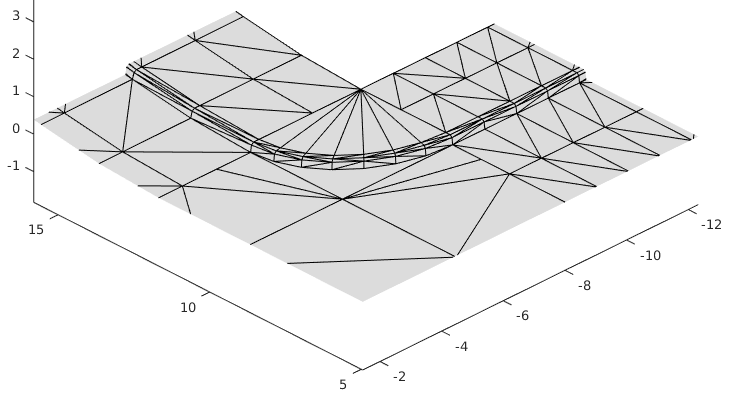
\includegraphics[width=0.6\linewidth]{Figures/mesh_dense}
	\caption{Porzione di \textit{mesh} particolarmente densa di triangoli.}
	\label{meshdense}
\end{figure}
\begin{figure}
	\centering
	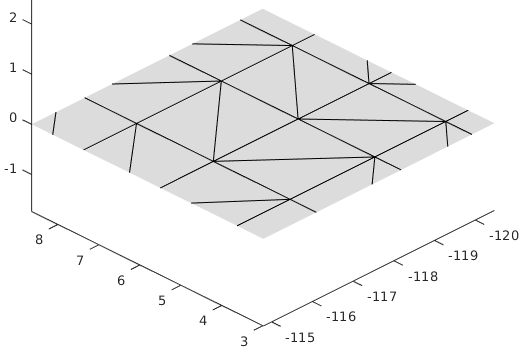
\includegraphics[width=0.6\linewidth]{Figures/mesh_notsodense}
	\caption{Porzione di \textit{mesh} non così particolarmente densa di triangoli.}
	\label{meshnotsodense}
\end{figure}
%
\clearpage
%
\begin{table}
	\centering
	\begin{tabular}{c|c|c|c|}
		\cline{2-4} 
		& \multicolumn{3}{c|}{\textbf{Modello di contatto}} \\
		\cline{2-4} 
		& \textbf{Rill} & \textbf{Ponderato sull'area} & \textbf{\textit{Mix}} \\ 
		\hline
		\multicolumn{1}{|c|}{$T_{totale}$ [ms]} & 116.543 & 121.249 & 106.058 \\ 
		\hline 
		\multicolumn{1}{|c|}{$T_{step}$ [ms]} & 0.0041621 & 0.00433017 & 0.00378765 \\ 
		\hline 
		\multicolumn{1}{|c|}{$\sigma$ [ms$^2$]} & 5.21719e-05 & 3.09234e-06 & 1.11754e-05 \\ 
		\hline
	\end{tabular}
	\\[0.5cm]
	Pneumatico 205/55R16\\
	Campionamenti = 28000\\
	Numero medio di triangoli sotto lo pneumatico = 11.4\\
	\textit{Switch} Rill $\triangleright$ Area a 10 triangoli
	\caption{Tempi per il modello di pneumatico a singolo disco \texttt{Tire::MagicFormula} nel caso di \textit{mesh} densa.}
	\label{MFcordolo}
\end{table}
\begin{table}
	\centering
	\begin{tabular}{c|c|c|c|c|c|}
		\cline{2-6} 
		& \multicolumn{2}{c|}{\textbf{Precisione}} &\multicolumn{3}{c|}{\textbf{Modello di contatto}} \\
		\cline{2-6} 
		& \textbf{Dischi} & \textbf{Punti} & \textbf{Campionamento} & \textbf{Ponderato sull'area} & \textbf{\textit{Mix}} \\ 
		\hline
		
		\multicolumn{1}{|c|}{$T_{step}$ [ms]} & 5 & 5 & 0.30604 & 0.027332 & 0.292775 \\ 
		\hline 
		\multicolumn{1}{|c|}{$\sigma$ [ms$^2$]} & 5 & 5 & 0.050355 & 0.0007717 & 0.076598 \\ 
		\hhline{======}
		
		\multicolumn{1}{|c|}{$T_{step}$ [ms]} & 10 & 5 & 0.31406 & 0.029972 & 0.30546 \\ 
		\hline 
		\multicolumn{1}{|c|}{$\sigma$ [ms$^2$]} & 10 & 5 & 0.0165893 & 0.000768059 & 0.038468 \\ 
		\hhline{======}
		
		\multicolumn{1}{|c|}{$T_{step}$ [ms]} & 5 & 10 & 0.38714 & 0.030945 & 0.37890 \\ 
		\hline 
		\multicolumn{1}{|c|}{$\sigma$ [ms$^2$]} & 5 & 10 & 0.039487 & 0.000744563 & 0.085648 \\ 
		\hhline{======}
		
		%%%
		\multicolumn{1}{|c|}{$T_{step}$ [ms]} & 10 & 10 & 0.40604 & 0.031138 & 0.316745 \\ 
		\hline 
		\multicolumn{1}{|c|}{$\sigma$ [ms$^2$]} & 10 & 10 & 0.0104055 & 0.000660589 & 0.0426783 \\ 
		\hhline{======}
		
		\multicolumn{1}{|c|}{$T_{step}$ [ms]} & 10 & 20 & 1.55412 & 0.0563041 & 1.17447 \\ 
		\hline 
		\multicolumn{1}{|c|}{$\sigma$ [ms$^2$]} & 10 & 20 & 0.142766 & 0.000214928 & 0.619357 \\ 
		\hhline{======}
		
		\multicolumn{1}{|c|}{$T_{step}$ [ms]} & 20 & 10 & 0.840434 & 0.0285447 & 0.651595 \\ 
		\hline 
		\multicolumn{1}{|c|}{$\sigma$ [ms$^2$]} & 20 & 10 & 0.0398545 & 5.12437e-05 & 0.193016 \\ 
		\hhline{======}
		 
		\multicolumn{1}{|c|}{$T_{step}$ [ms]} & 20 & 20 & 3.46259 & 0.0587258 & 2.73157 \\ 
		\hline 
		\multicolumn{1}{|c|}{$\sigma$ [ms$^2$]} & 20 & 20 & 0.692889 & 0.000257929 & 3.51893 \\
		\hline
	\end{tabular}
	\\[0.5cm]
	Pneumatico 205/55R16\\
	Campionamenti = 28000\\
	Numero medio di triangoli sotto lo pneumatico = 11.4\\
	\textit{Switch} Campionamento $\triangleright$ Area a 10 triangoli
	\caption{Tempi per il modello di pneumatico a più dischi \texttt{Tire::MultiDisk} nel caso di \textit{mesh} densa.}
	\label{MDcordolo}
\end{table}
%
\clearpage
%
\begin{table}
	\centering
	\begin{tabular}{c|c|c|c|}
		\cline{2-4} 
		& \multicolumn{3}{c|}{\textbf{Modello di contatto}} \\
		\cline{2-4} 
		& \textbf{Rill} & \textbf{Ponderato sull'area} & \textbf{\textit{Mix}} \\ 
		\hline 
		\multicolumn{1}{|c|}{$T_{totale}$ [ms]} & 64.15 & 46.44 & 54.269 \\ 
		\hline 
		\multicolumn{1}{|c|}{$T_{step}$ [ms]} & 0.00229099 & 0.00165851 & 0.00193811 \\ 
		\hline 
		\multicolumn{1}{|c|}{$\sigma$ [ms$^2$]} & 3.92268e-06 & 4.39344e-06 & 5.825e-06 \\
		\hline 
	\end{tabular}
	\\[0.5cm]
	Pneumatico 205/55R16\\
	Campionamenti = 28000\\
	Numero medio di triangoli sotto lo pneumatico = 3.2\\
	\textit{Switch} Rill $\triangleright$ Area a 3 triangoli
	\caption{Tempi per il modello di pneumatico a singolo disco \texttt{Tire::MagicFormula} nel caso di \textit{mesh} poco densa.}
	\label{MFpiano}
\end{table}
\begin{table}
	\centering
	\begin{tabular}{c|c|c|c|c|c|}
		\cline{2-6} 
		& \multicolumn{2}{c|}{\textbf{Precisione}} &\multicolumn{3}{c|}{\textbf{Modello di contatto}} \\
		\cline{2-6} 
		& \textbf{Dischi} & \textbf{Punti} & \textbf{Campionamento} & \textbf{Ponderato sull'area} & \textbf{\textit{Mix}} \\ 
		\hline
		
		\multicolumn{1}{|c|}{$T_{step}$ [ms]} & 5 & 5 & 0.29604 & 0.010375 & 0.020880 \\ 
		\hline 
		\multicolumn{1}{|c|}{$\sigma$ [ms$^2$]} & 5 & 5 & 0.00364537 & 0.00734568 & 0.0027406 \\ 
		\hhline{======}
		
		\multicolumn{1}{|c|}{$T_{step}$ [ms]} & 10 & 5 & 0.31406 & 0.015352 & 0.027446 \\ 
		\hline 
		\multicolumn{1}{|c|}{$\sigma$ [ms$^2$]} & 10 & 5 & 0.0174863 & 0.000436738 & 0.0047837 \\ 
		\hhline{======}
		
		\multicolumn{1}{|c|}{$T_{step}$ [ms]} & 5 & 10 & 0.42839 & 0.01972 & 0.038590 \\ 
		\hline 
		\multicolumn{1}{|c|}{$\sigma$ [ms$^2$]} & 5 & 10 & 0.027645 & 0.0045783 & 0.007463 \\ 
		\hhline{======}
		
		%%%
		\multicolumn{1}{|c|}{$T_{step}$ [ms]} & 10 & 10 & 0.213785 & 0.0115888 & 0.0111662 \\ 
		\hline 
		\multicolumn{1}{|c|}{$\sigma$ [ms$^2$]} & 10 & 10 & 0.0021398 & 1.73799e-05 & 2.52509e-05 \\
		\hhline{======}

		\multicolumn{1}{|c|}{$T_{step}$ [ms]} & 10 & 20 & 0.902904 & 0.0210344 & 0.0222986 \\ 
		\hline 
		\multicolumn{1}{|c|}{$\sigma$ [ms$^2$]} & 10 & 20 & 0.0444643 & 4.91353e-05 & 0.000116275 \\ 
		\hhline{======}
		
		\multicolumn{1}{|c|}{$T_{step}$ [ms]} & 20 & 10 & 0.481218 & 0.0114461 & 0.0112381 \\ 
		\hline 
		\multicolumn{1}{|c|}{$\sigma$ [ms$^2$]} & 20 & 10 & 0.0115384 & 2.87254e-05 & 1.70045e-05 \\ 
		\hhline{======}
		
		\multicolumn{1}{|c|}{$T_{step}$ [ms]} & 20 & 20 & 1.88533 & 0.019253 & 0.0193953 \\ 
		\hline 
		\multicolumn{1}{|c|}{$\sigma$ [ms$^2$]} & 20 & 20 & 0.142808 & 2.87459e-05 & 3.20608e-05 \\ 
		\hline
	\end{tabular}
	\\[0.5cm]
	Pneumatico 205/55R16\\
	Campionamenti = 28000\\
	Numero medio di triangoli sotto lo pneumatico = 3.2\\
	\textit{Switch} Campionamento $\triangleright$ Area a 3 triangoli
	\caption{Tempi per il modello di pneumatico a più dischi \texttt{Tire::MultiDisk} nel caso di \textit{mesh} poco densa.}
	\label{MDpiano}
\end{table}
%
\clearpage
\noindent
Testando il modello al simulatore è stato possibile valutare la sua complessità computazionale. Le specifiche tecniche di questo simulatore sono:
\begin{itemize}
	%\item sistema operativo: 64bit Concurrent Real-Time RedHawk 7.5 (CentOS 7.5 + RedHawk 4.9.98 Real-Time Kernel);
	\item memoria RAM: 32 GB;
	\item processore: Intel Xeon(R) 3.40 GHz (16 \textit{cores});
	\item scheda grafica: Nvidia GeForce GTX 680.
\end{itemize}
I tempi rilevati per il modello di pneumatico a singolo disco \texttt{Tire::MagicFormula} sono riportati nella Tabella \ref{MF}. Analogamente, i tempi rilevati per il modello di pneumatico a più dischi \texttt{Tire::MultiDisk} sono riportati nella Tabella \ref{MD}.
%
\begin{table}
	\centering
	\begin{tabular}{c|c|c|}
		\cline{2-3} 
		& \multicolumn{2}{c|}{\textbf{Modello di contatto}} \\
		\cline{2-3} 
		& \textbf{Ponderato sull'area} & \textbf{\textit{Mix}} \\ 
		\hline
		\multicolumn{1}{|c|}{$T_{step}$ [$\mu$s]} & 9.6688 & 9.7658 \\ 
		\hline 
		\multicolumn{1}{|c|}{$\sigma$ [$\mu$s$^2$]} & 1.4018 & 1.4983 \\ 
		\hline
	\end{tabular}
	\\[0.5cm]
	Pneumatico 250/55R11\\
	Campionamenti = 30000\\
	\textit{Switch} Rill $\triangleright$ Area a 10 triangoli
	\caption{Tempi sul simulatore per il modello di pneumatico a singolo disco \texttt{Tire::MagicFormula}.}
	\label{MF}
\end{table}
%
\begin{table}
	\centering
	\begin{tabular}{c|c|c|c|c|}
		\cline{2-5} 
		& \multicolumn{2}{c|}{\textbf{Precisione}} &\multicolumn{2}{c|}{\textbf{Modello di contatto}} \\
		\cline{2-5} 
		& \textbf{Dischi} & \textbf{Punti} & \textbf{Ponderato sull'area} & \textbf{\textit{Mix}} \\ 
		\hline
		\multicolumn{1}{|c|}{$T_{step}$ [$\mu$s]} & 5 & 5 & 24.5736 & 39.6069 \\ 
		\hline 
		\multicolumn{1}{|c|}{$\sigma$ [$\mu$s$^2$]} & 10 & 5 & 42.6262 & 439.6915 \\ 
		\hhline{=====}
		
		\multicolumn{1}{|c|}{$T_{step}$ [$\mu$s]} & 5 & 10 & 24.6686 & 55.7135 \\ 
		\hline 
		\multicolumn{1}{|c|}{$\sigma$ [$\mu$s$^2$]} & 10 & 10 & 41.4114 & 479.8682 \\ 
		\hline
	\end{tabular}
	\\[0.5cm]
	Pneumatico 250/55R11\\
	Campionamenti = 30000\\
	\textit{Switch} Campionamento $\triangleright$ Area a 10 triangoli
	\caption{Tempi sul simulatore per il modello di pneumatico a più dischi \texttt{Tire::MultiDisk}.}
	\label{MD}
\end{table}

\chapter{Conclusioni e possibili sviluppi}
\label{Conclusione}
%
I modelli sviluppati, nelle corrette condizioni di lavoro, soddisfano il vincolo del tempo reale imposto dalle condizioni di utilizzo. Il tempo di calcolo sull'\textit{hardware} del simulatore professionale si traduce in un ciclo di lavoro del ??\% circa, garantendo quindi un ampio margine di sicurezza e dando la possibilità di aumentare la precisione del modello attraverso l'implementazione di modelli più complessi.

I modelli di contatto sviluppati garantiscono un tempo di esecuzione basso. In generale per qualità dell'\textit{output} generato e per tempo di compitazione il modello di contatto ponderato sull'area d'intersezione è da preferire. Esso infatti permette di rilevare ostacoli anche al di fuori dell'impronta di contatto garantendo quindi una descrizione qualitativamente maggiore del contatto tra lo pneumatico e la strada. Inoltre è opportuno settare lo \textit{switch} tra un modello di contatto e l'altro indicaticamente quanto i triangoli all'interno dell'ombra di contatto sono maggiori del prodotto tra il numero di dischi e il numero di punti di campionamento associati ad ogni disco. Considerando dunque le finalità principali e i test effettuati sul modello sviluppato, possiamo affermare la sua validità per i campi di utilizzo previsti.

Un punto critico sul quale è opportuno porre particolare attenzione è la rappresentazione del terreno. I \textit{file} \ac{RDF} hanno una struttura dati molto poco formale e solida. La mancanza di uno standard universalmente riconosciuto per questo formato rende impossibile implementare un \textit{parser} sufficientemente efficiente e la stabile per tutte le occasioni.

\begin{figure}
	\centering
	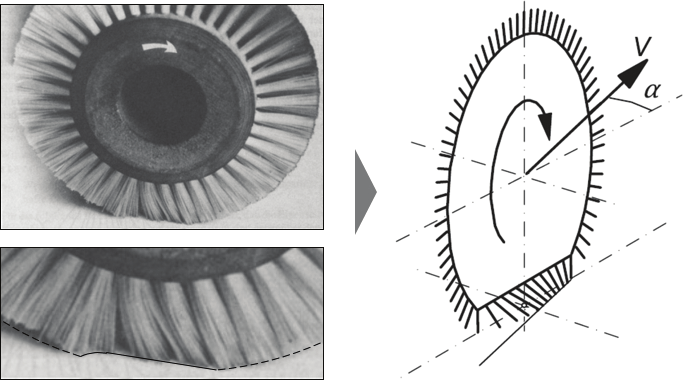
\includegraphics[width=0.7\linewidth]{Figures/brush_model}
	\caption{Schema strutturale del modello "a spazzola" (\textit{brush model}). }
	\label{brushmodel}
\end{figure}

Infine, bisogna certamente notare che la rappresentazione dello pneumatico è basato sul modello di Pacejka, ovvero un modello semi-empirico che non tiene conto dei fenomeni transitori. Sarà quindi una scelta obbligata passare ad una rappresentazione dello pneumatico mediante un modello fisico. Quest'ultimo, infatti, a seconda del grado di complessità, può tenere in considerazione alcuni dei fenomeni transitori che maggiormente influenzano la manovrabilità del veicolo. I modelli fisici sono quindi anche molto complessi. Lo pneumatico è modellato da divesi anelli circolari con punti di massa accoppiati anche in direzione laterale. Si tiene quindi conto del contatto in più punti e della distribuzione della pressione su tutta la larghezza della cintura. Importante sarà quindi valutare la possibilità di poter parallelizzare i processi di calcolo per diminuire i tempi di esecuzione.
%\chapter{A Chapter of Examples}
\label{chapter1}

\section{A Table}

\begin{table}[h]
\centering
\begin{tabular}{rcc}
\toprule \emph{Feature} & \textsc{Misuse-based} &
\textsc{Anomaly-based}\\
    
\midrule Modeled activity: & Malicious & Normal\\
Detection method: & Matching & Deviation\\
Threats detected: & Known & Any\\
False negatives: & High & Low\\
False positives: & Low & High\\
Maintenance cost: & High & Low\\
Attack desc.: & Accurate & Absent\\
System design: & Easy & Difficult\\
\bottomrule
\end{tabular}
\caption[Duality between misuse- and anomaly-based intrusion detection techniques.]{Duality between misuse- and anomaly-based intrusion detection techniques. Note that, an anomaly-based \acp{CAM} can detect ``Any'' threat, under the assumption that an attack always generates a deviation in the modeled activity.}
\label{tab:misuse-vs-anomaly}
\end{table}

%------------------------------------------------

\section{Code}

\begin{pseudoc}
  /* ... */ cd['<'] = {0.1, 0.11} cd['a'] = {0.01, 0.2} cd['b'] =
  {0.13, 0.23} /* ... */

  b = decode(arg3_value);
  
  if ( !(cd['c'][0] < count('c', b) < cd['c'][1]) ||\
       !(cd['<'][0] < count('<', b) < cd['<'][1]) ||\
       ... || ...)  fire_alert("Anomalous content detected!");
  /* ... */
\end{pseudoc}

%------------------------------------------------

\section{A Sideways Table}

\clearpage
\begin{sidewaystable}
\renewcommand{\arraystretch}{1.5} \centering
\begin{tabular}{rcccccc}
\toprule \textsc{Approach} & \textsc{Time} & \textsc{Header} &
\textsc{Payload} & \textsc{Stochastic} & \textsc{Determ.} & \textsc{Clustering}\\
\midrule \cite{phad} & & $\bullet$ & & & & $\bullet$ \\
\cite{kruegel:sac2002:anomaly} & & $\bullet$ & $\bullet$ & $\bullet$ & & \\
\cite{protocolanom} & & $\bullet$ & & $\bullet$ & $\bullet$ & \\
\cite{ramadas} & & & $\bullet$ & & & $\bullet$ \\
\cite{rules-payl} & $\bullet$ & & $\bullet$ & & $\bullet$ & \\
\cite{zanero-savaresi} & & $\bullet$ & $\bullet$ & & & $\bullet$ \\
\cite{wang:raid2004:payl} & & & $\bullet$ & $\bullet$ & & \\
\cite{zanero-pattern} & & $\bullet$ & $\bullet$ & & & $\bullet$ \\
\cite{DBLP:conf/iwia/BolzoniEHZ06} & & $\bullet$ & $\bullet$ & & & $\bullet$ \\
\cite{wang:raid2006:anagram} & & & $\bullet$ & $\bullet$ & & \\
\bottomrule
\end{tabular}
\caption{Taxonomy of the selected state of the art approaches for network-based anomaly detection.}
\label{tab:network-sota-taxonomy}
\end{sidewaystable}
\clearpage

%------------------------------------------------

\section{A Figure}

\begin{figure}[h]
\centering
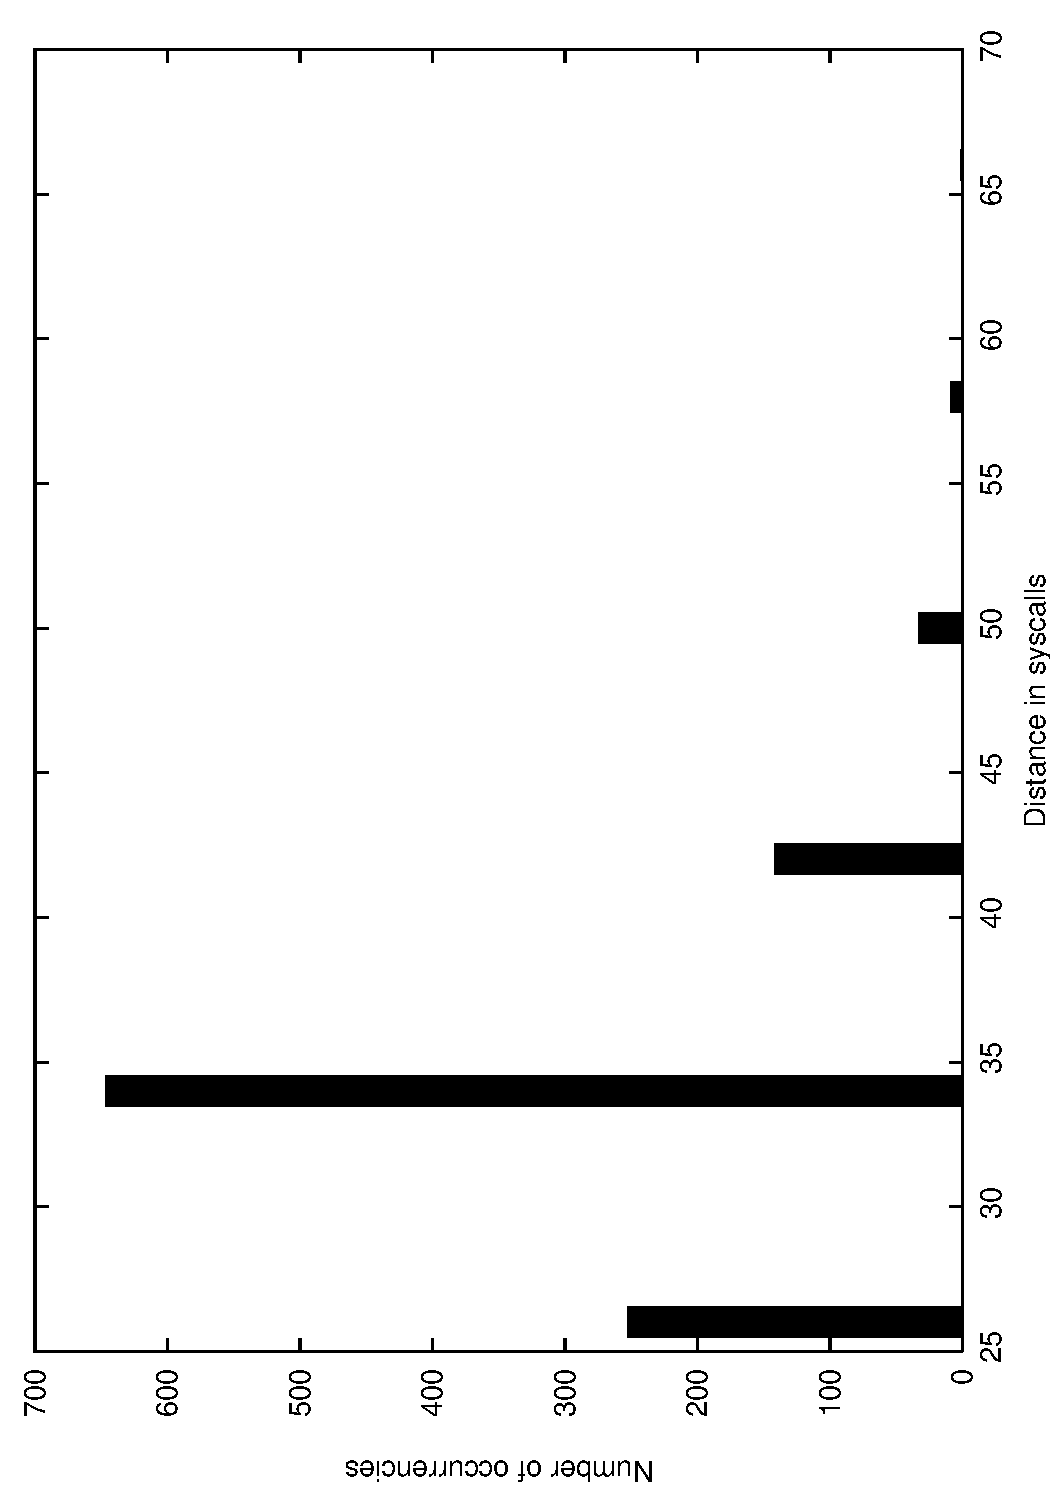
\includegraphics[angle=-90,width=.8\textwidth]{Figures/telnet.pdf}
\caption{\texttt{telnetd}: distribution of the number of other system calls among two \texttt{execve} system calls (i.e., distance between two consecutive \texttt{execve}).}
\label{fig:exectelnet}
\end{figure}

%------------------------------------------------

\section{Bulleted List}

\begin{itemize}
\item $O = $``Intrusion'', $\neg O =$``Non-intrusion'';
\item $A = $``Alert reported'', $\neg A =$``No alert reported''.
\end{itemize}

%------------------------------------------------

\section{Numbered List}

\begin{enumerate}
\item $O = $``Intrusion'', $\neg O =$``Non-intrusion'';
\item $A = $``Alert reported'', $\neg A =$``No alert reported''.
\end{enumerate}

%------------------------------------------------

\section{A Description}

\begin{description}
\item[Time] refers to the use of \emph{timestamp} information, extracted from network packets, to model normal packets. For example, normal packets may be modeled by their minimum and maximum inter-arrival time.

\end{description}

%------------------------------------------------

\section{An Equation}

\begin{equation}
d_a(i,j) := \left\{
\begin{array}{lll}
K_a + \alpha_{a} \delta_{a}(i,j) & \mbox{if the elements are different} \\
0 & \mbox{otherwise}
\end{array}
\right.
\label{eq:distfunction}
\end{equation}

%------------------------------------------------

\section{A Theorem, Proposition \& Proof}

\begin{thm}
$a^2 + b^2 = c^2$
\end{thm}

\begin{prop}
$3 + 3 = 6$
\end{prop}

\begin{proof}
For any finite set $\{p_1,p_2,...,p_n\}$ of primes, consider $m = p_1p_2...p_n+1$. If $m$ is prime it is not in the set since $m > p_i$ for all $i$. If $m$ is not prime it has a prime divisor $p$. If $p$ is one of the $p_i$ then $p$ is a divisor of $p_1p_2...p_n$ and hence is a divisor of $(m - p_1p_2...p_n) = 1$, which is impossible; so $p$ is not in the set. Hence a finite set $\{p_1,p_2,...,p_n\}$ cannot be the collection of all primes.
\end{proof}

%------------------------------------------------

\section{Definition}

\begin{definition}[Anomaly-based \ac{CAM}]
An \emph{anomaly-based \ac{CAM}} is a type of \ac{CAM} that generate alerts $\mathbb{A}$ by relying on normal activity profiles.
\end{definition}

%------------------------------------------------

\section{A Remark}

\begin{rem}
Although the network stack implementation may vary from system to system (e.g., \textsf{Windows} and \textsf{Cisco} platforms have different implementation of \ac{CAM}).
\end{rem}

%------------------------------------------------

\section{An Example}

\begin{example}[Misuse \emph{vs.} Anomaly]\label{ex:misuse-vs-anomaly}
A misuse-based system $M$ and an anomaly-based system $A$ process the same log containing a full dump of the system calls invoked by the kernel of an audited machine. Log entries are in the form:

\begin{center}\small
\begin{verbatim} <function_name>(<arg1_value>, <arg2_value>, ...)
\end{verbatim}
\end{center}
\end{example}

%------------------------------------------------

\section{Note}

\begin{note}[Inspection layer]\label{note:network-stack-standardized}
Although the network stack implementation may vary from system to system (e.g., \textsf{Windows} and \textsf{Cisco} platforms have different implementation of \ac{CAM}), it is important to underline that the notion of IP, TCP, HTTP \emph{packet} is well defined in a system-agnostic way, while the notion of \emph{operating system activity} is rather vague and by no means standardized.
\end{note}


\appendix
\chapter{Convenzioni e Notazioni}
\label{Notazioni}
%
\subsection{Sistemi di Riferimento}
La convenzione utilizzata per definire gli assi del sistema di riferimento della vettura è la \ac{ISO} 8855.

\begin{figure}[h!]
	\centering
	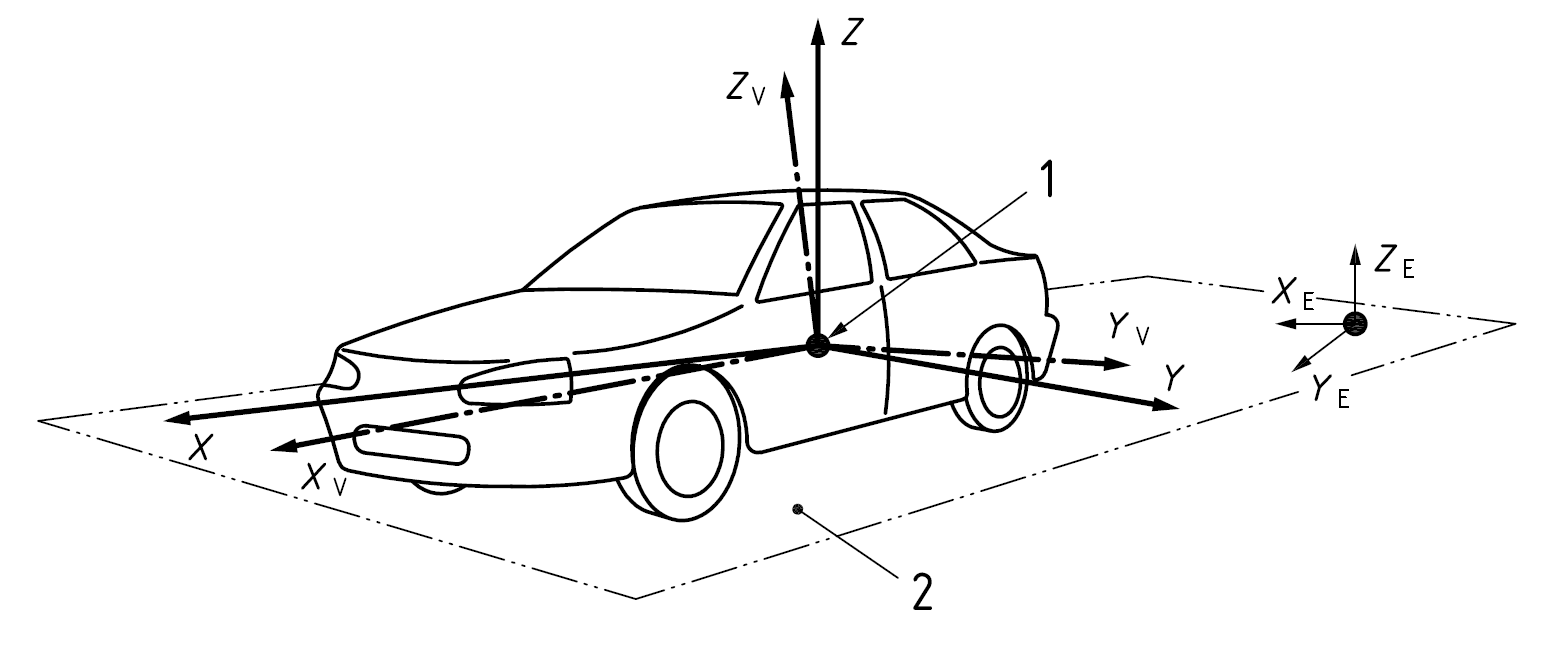
\includegraphics[width=0.8\linewidth]{Figures/iso_convention}
	\caption{Rappresentazione degli assi del sistema di riferimento della vettura secondo la convenzione ISO-V.}
	Da: \citeauthor{Ginebra}, \citetitle{Ginebra}.
	\label{isoconventionv}
\end{figure}

\noindent
Il sistema di riferimento della ruota è conforme alla convenzione \ac{ISO}-V, la cui disposizione degli assi è illustrata nella \figurename{ \ref{isoconventionc}}. L'origine del sistema di riferimento del vettore ruota è posta in corrispondenza del centro della ruota mentre posizione e orientamento relativi rispetto al sistema di riferimento del telaio sono definiti attraverso il modello della sospensione descritto in \cite{Larcher}.

\begin{figure}[h!]
	\centering
	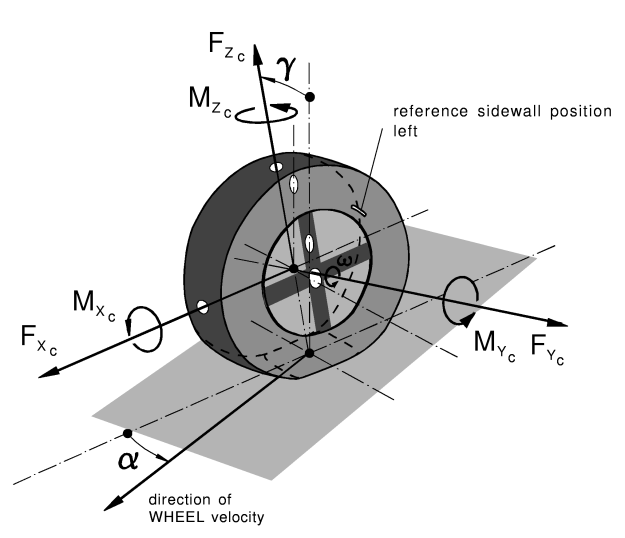
\includegraphics[width=0.6\linewidth]{Figures/iso_convention_wheel}
	\caption{Rappresentazione degli assi  del sistema di riferimento dello pneumatico secondo la convenzione ISO-C.}
	Da: Documentazione \texttt{MFeval}.
	\label{isoconventionc}
\end{figure}
%
\subsection{Matrice di Trasformazione}
Per descrivere sia l'orientamento che la posizione di un sistema di assi nello spazio, viene introdotta la matrice roto-traslazione, chiamata anche matrice di trasformazione. Questa notazione permette di impiegare le operazioni matrice-vettore per l'analisi di posizione, velocità e accelerazione. La forma generale di una matrice di trasformazione è del tipo:
%
\begin{equation}
T_m = \left[
\begin{array}{ccc|c}
& & & O_{mx}\\
\multicolumn{3}{c|}{\multirow{3}{*}{\raisebox{20mm}{\scalebox{1.5}{$[R_m]$}}}} & O_{my}\\
& & & O_{mz}\\ \hline
0 & 0 & 0 & 1
\end{array}\right]
\end{equation}\\
%
dove $R_m$ è la matrice di rotazione $3 \times 3$ del sistema di riferimento in movimento e $O_{mx}$, $O_{my}$ e $O_{mz}$ sono le coordinate della sua origine nel sistema di riferimento assoluto o nativo.

L'introduzione dell'elemento fittizio 1 nel vettore della posizione di origine e la successiva spaziatura interna zero della matrice rende possibili le moltiplicazioni matrice-vettore, rendendo la matrice di trasformazione una notazione compatta e conveniente per la descrizione dei sistemi di riferimento. Si noti che per i vettori, le informazioni traslazionali vengono trascurate imponendo l'elemento fittizio pari a 0.
%
\chapter{Documentazione della libreria \texttt{TireGround}}
\label{Documentation}
%
\texttt{Doxygen} è un \textit{software} comunemente utilizzato per generare documentazione direttamente dalle annotazioni nei file \texttt{C++}. Questo \textit{tool} supporta anche altri linguaggi di programmazione popolari come \texttt{C}, \texttt{Objective-C}, \texttt{C\#}, \texttt{PHP},  \texttt{Java},  \texttt{Python}, \texttt{Fortran},  \texttt{VHDL},  \texttt{Tcl} e in una certa misura  \texttt{D}.

\texttt{Doxygen} può essere utile per i seguenti motivi.
\begin{itemize}
	\item Può generare una documentazione da utilizzare \textit{online} (in \texttt{HTML}) e/o un manuale di riferimento \textit{offline} (in \LaTeX) da una serie di \textit{file} sorgente oppurtunamente annotati. C'è anche il supporto per generare \textit{output} in \texttt{RTF} (MicroSoft Word), \texttt{PostScript}, \texttt{PDF} con \textit{hyperlink} e \texttt{HTML} compresso. La documentazione viene estratta direttamente dalle fonti, il che rende molto più semplice mantenere la documentazione coerente con il codice sorgente.
	\item È possibile configurare \texttt{doxygen} per estrarre la struttura del codice da \textit{file} sorgente non documentati. Questo è molto utile per analizzare rapidamente ed efficaciemente i \textit{file} sorgente di grandi dimensioni. Doxygen può anche visualizzare le relazioni tra i vari elementi mediante grafici di dipendenza, diagrammi di ereditarietà e diagrammi di collaborazione, tutti generati automaticamente.
\end{itemize}
\texttt{Doxygen} è sviluppato su Mac OS X e Linux, ma è configurato per essere altamente portabile. Di conseguenza, funziona anche con la maggior parte degli altri sistemi Unix. Inoltre, sono disponibili eseguibili per Windows.

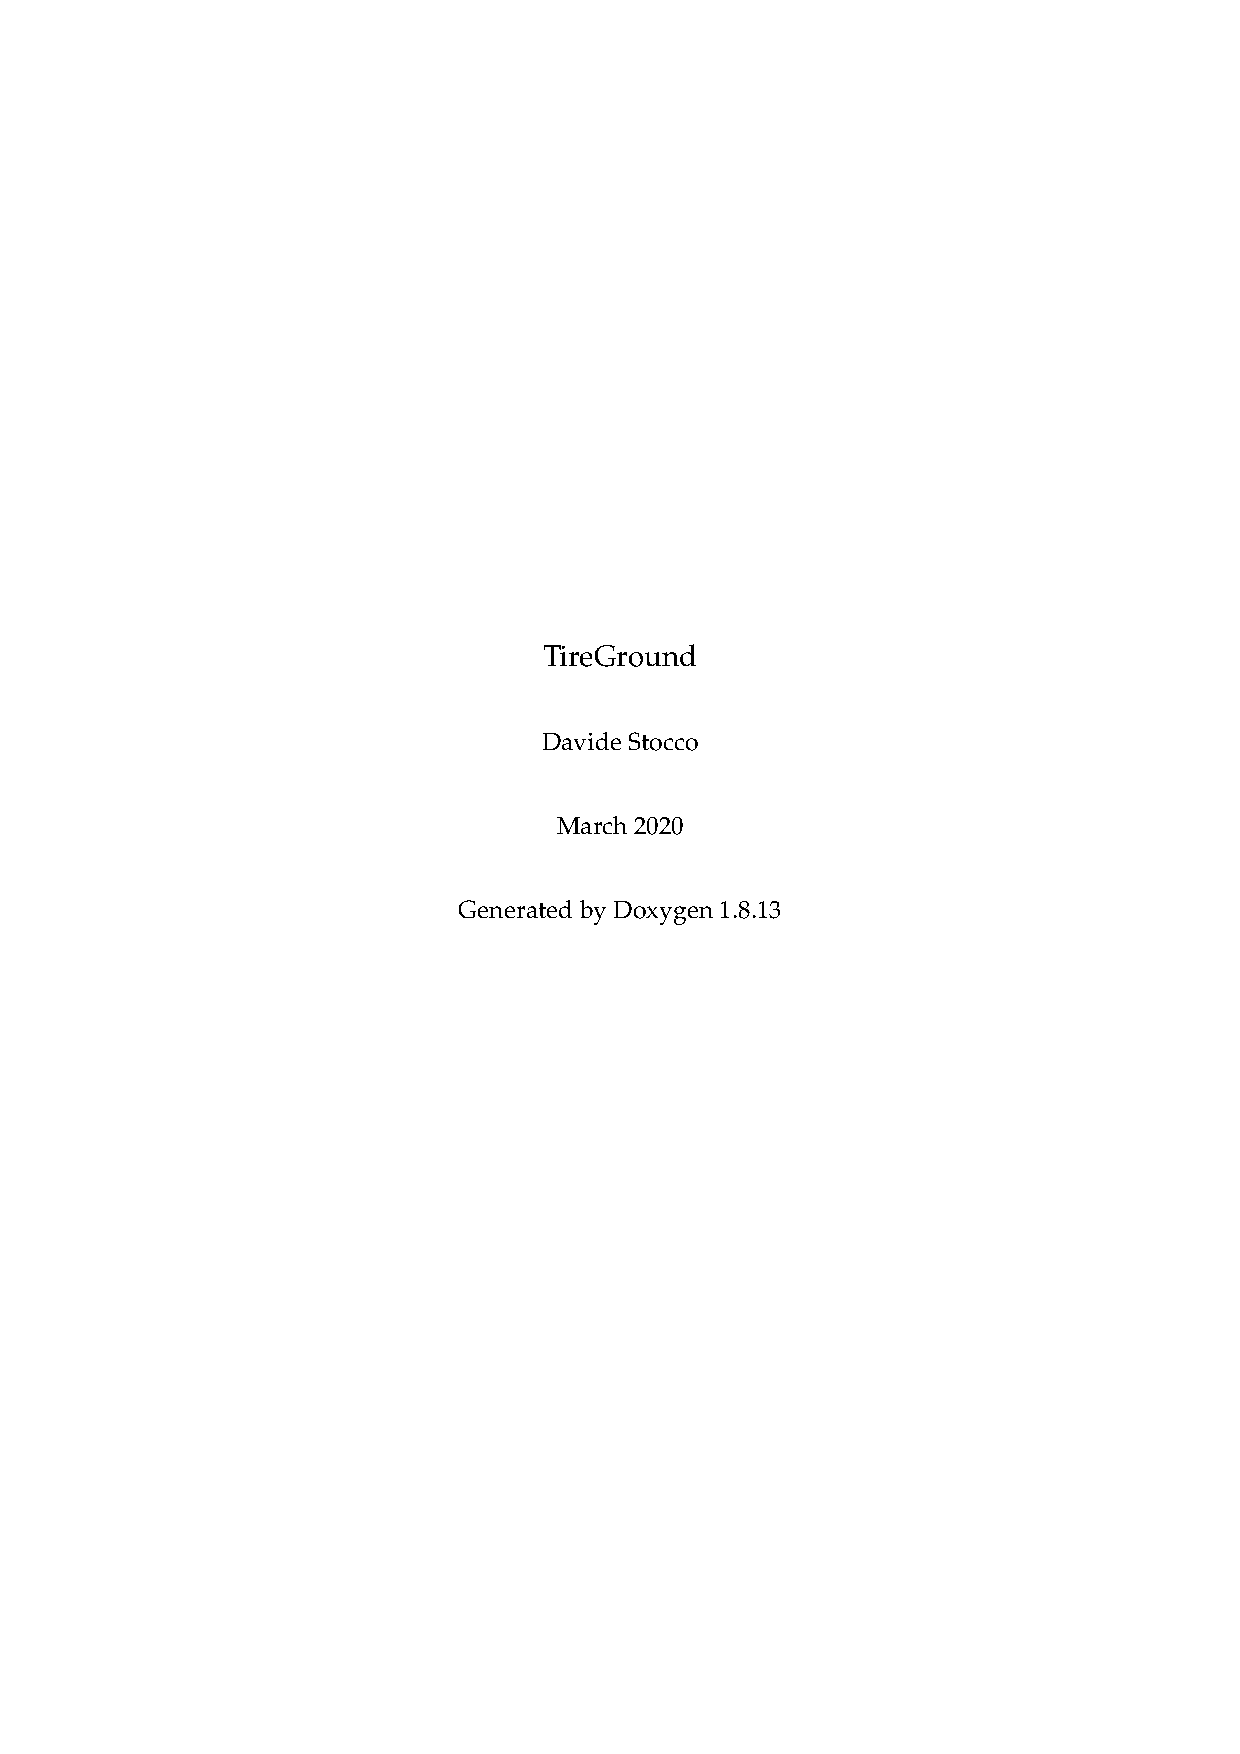
\includepdf[pages=-, offset=10mm 0mm]{refman.pdf}

\chapter{Codice dei Tests}
\label{TestsCode}
%
\section{Tests Geometrici}
%
\subsection{Geometry-test1.cc}
\renewcommand{\baselinestretch}{1.0}
\lstinputlisting{../TireGround/tests/Geometry-test1.cc}
\renewcommand{\baselinestretch}{1.25}
%
\subsection{Geometry-test2.cc}
\renewcommand{\baselinestretch}{1.0}
\lstinputlisting{../TireGround/tests/Geometry-test2.cc}
\renewcommand{\baselinestretch}{1.25}
%
\subsection{Geometry-test3.cc}
\renewcommand{\baselinestretch}{1.0}
\lstinputlisting{../TireGround/tests/Geometry-test3.cc}
\renewcommand{\baselinestretch}{1.25}
%
\subsection{Geometry-test4.cc}
\renewcommand{\baselinestretch}{1.0}
\lstinputlisting{../TireGround/tests/Geometry-test4.cc}
\renewcommand{\baselinestretch}{1.25}
%
\section{Tests per il Modello a Singolo Disco}
%
\subsection{MagicFormula-test1.cc}
\renewcommand{\baselinestretch}{1.0}
\lstinputlisting{../TireGround/tests/MagicFormula-test1.cc}
\renewcommand{\baselinestretch}{1.25}
%
\subsection{MagicFormula-test2.cc}
\renewcommand{\baselinestretch}{1.0}
\lstinputlisting{../TireGround/tests/MagicFormula-test2.cc}
\renewcommand{\baselinestretch}{1.25}
%
\section{Tests per il Modello a più Dischi}
%
\subsection{MultiDisk-test1.cc}
\renewcommand{\baselinestretch}{1.0}
\lstinputlisting{../TireGround/tests/MultiDisk-test1.cc}
\renewcommand{\baselinestretch}{1.25}
%
\subsection{MultiDisk-test2.cc}
\renewcommand{\baselinestretch}{1.0}
\lstinputlisting{../TireGround/tests/MultiDisk-test2.cc}
\renewcommand{\baselinestretch}{1.25}

\backmatter
\chapterstyle{default} % Change the style of the Chapter header to that defined in structure.tex

%----------------------------------------------------------------------------------------
%	BIBLIOGRAPHY
%----------------------------------------------------------------------------------------

\printbibliography

%----------------------------------------------------------------------------------------
%	INDEX
%----------------------------------------------------------------------------------------

\printindex % Print the index

%----------------------------------------------------------------------------------------

\end{document}
